% !TeX spellcheck = hu_HU
% !TeX encoding = UTF-8
% !TeX program = xelatex
% TODO Change language to en_GB (recommended) or en_US for English documents
\documentclass[11pt,a4paper,oneside]{report}             % Single-side
%\documentclass[11pt,a4paper,twoside,openright]{report}  % Duplex

% thanks to http://tex.stackexchange.com/a/47579/71109
\usepackage{ifxetex}
\usepackage{ifluatex}
\newif\ifxetexorluatex % a new conditional starts as false
%\ifnum 0\ifxetex 1\fi\ifluatex 1\fi>0
%   \xetexorluatextrue
%\fi

\ifxetexorluatex
  \usepackage{fontspec}
\else
  \usepackage[T1]{fontenc}
  \usepackage[utf8]{inputenc}
  \usepackage[lighttt]{lmodern}
  \ttfamily\DeclareFontShape{T1}{lmtt}{m}{it}{<->sub*lmtt/m/sl}{}
\fi
\usepackage[ruled,linesnumbered]{algorithm2e}
\usepackage[english,magyar]{babel} % Alapértelmezés szerint utoljára definiált nyelv lesz aktív, de később külön beállítjuk az aktív nyelvet.

\usepackage{emptypage} % omit page number on empty pages

%\usepackage{cmap}
\usepackage{amsfonts,amsmath,amssymb} % Mathematical symbols.
%\usepackage[ruled,boxed,resetcount,linesnumbered]{algorithm2e} % For pseudocodes. % beware: this is not compatible with LuaLaTeX, see http://tex.stackexchange.com/questions/34814/lualatex-and-algorithm2e
\usepackage{booktabs} % For publication quality tables for LaTeX
\usepackage{graphicx}

%\usepackage{fancyhdr}
%\usepackage{lastpage}

\usepackage{anysize}
%\usepackage{sectsty}
\usepackage{setspace} % For setting line spacing

\usepackage[unicode]{hyperref} % For hyperlinks in the generated document.
\usepackage{xcolor}
\usepackage{listings} % For source code snippets.

\usepackage[amsmath,thmmarks]{ntheorem} % Theorem-like environments.

\usepackage[hang]{caption}

\singlespacing

\newcommand{\selecthungarian}{
	\selectlanguage{magyar}
	\setlength{\parindent}{2em}
	\setlength{\parskip}{0em}
	\frenchspacing
}

\newcommand{\selectenglish}{
	\selectlanguage{english}
	\setlength{\parindent}{0em}
	\setlength{\parskip}{0.5em}
	\nonfrenchspacing
	\renewcommand{\figureautorefname}{Figure}
	\renewcommand{\tableautorefname}{Table}
	\renewcommand{\partautorefname}{Part}
	\renewcommand{\chapterautorefname}{Chapter}
	\renewcommand{\sectionautorefname}{Section}
	\renewcommand{\subsectionautorefname}{Section}
	\renewcommand{\subsubsectionautorefname}{Section}
}

\usepackage[numbers]{natbib}
\usepackage{xspace}

\usepackage{caption}
\usepackage{subcaption}


%TODO Set the main variables
\newcommand{\vikszerzoVezeteknev}{Barcsa-Szabó}
\newcommand{\vikszerzoKeresztnev}{Áron}

\newcommand{\vikkonzulensAMegszolitas}{}
\newcommand{\vikkonzulensAVezeteknev}{Farkas}
\newcommand{\vikkonzulensAKeresztnev}{Rebeka}

\newcommand{\vikkonzulensBMegszolitas}{dr. }
\newcommand{\vikkonzulensBVezeteknev}{Molnár}
\newcommand{\vikkonzulensBKeresztnev}{Vince}

\newcommand{\vikkonzulensCMegszolitas}{dr. }
\newcommand{\vikkonzulensCVezeteknev}{Vörös}
\newcommand{\vikkonzulensCKeresztnev}{András}

\newcommand{\vikcim}{Interactive Learning for Model-Based Software Engineering} % Cím
\newcommand{\viktanszek}{\bmemit} % Tanszék
\newcommand{\vikdoktipus}{\bsc} % Dokumentum típusa (\bsc vagy \msc)
\newcommand{\vikmunkatipusat}{szakdolgozatot} % a "hallgató nyilatkozat" részhez: szakdolgozatot vagy diplomatervet

%--------------------------------------------------------------------------------------
% TDK-specifikus változók
%--------------------------------------------------------------------------------------
\newcommand{\tdkszerzoB}{Balázs Várady} % Második szerző neve; hagyd üresen, ha egyedül írtad a TDK-t.
\newcommand{\tdkev}{2020} % A dolgozat írásának éve (pl. "2014") (Ez OTDK-nál eltérhet az aktuális évtől.)

% További adatok az OTDK címlaphoz (BME-s TDK-hoz nem kell kitölteni)
\newcommand{\tdkevfolyamA}{IV} % Első szerző évfolyama, római számmal (pl. IV).
\newcommand{\tdkevfolyamB}{III} % Második szerző évfolyama, római számmal (pl. III).
\newcommand{\tdkkonzulensbeosztasA}{egyetemi tanár} % Első konzulens beosztása (pl. egyetemi docens)
\newcommand{\tdkkonzulensbeosztasB}{doktorandusz} % Második konzulens beosztása (pl. egyetemi docens)

\newcommand{\szerzoMeta}{\vikszerzoVezeteknev{} \vikszerzoKeresztnev} % egy szerző esetén
%\newcommand{\szerzoMeta}{\vikszerzoVezeteknev{} \vikszerzoKeresztnev, \tdkszerzoB} % két szerző esetén

% Beállítások magyar nyelvű dolgozathoz
%%--------------------------------------------------------------------------------------
% Elnevezések
%--------------------------------------------------------------------------------------
\newcommand{\bme}{Budapesti Műszaki és Gazdaságtudományi Egyetem}
\newcommand{\vik}{Villamosmérnöki és Informatikai Kar}

\newcommand{\bmemit}{Méréstechnika és Információs Rendszerek Tanszék}

\newcommand{\keszitette}{Készítette}
\newcommand{\konzulens}{Konzulens}

\newcommand{\bsc}{Szakdolgozat}
\newcommand{\msc}{Diplomaterv}
\newcommand{\tdk}{TDK dolgozat}
\newcommand{\bsconlab}{BSc Önálló laboratórium}
\newcommand{\msconlabi}{MSc Önálló laboratórium 1.}
\newcommand{\msconlabii}{MSc Önálló laboratórium 2.}

\newcommand{\pelda}{Példa}
\newcommand{\definicio}{Definíció}
\newcommand{\tetel}{Tétel}

\newcommand{\bevezetes}{Bevezetés}
\newcommand{\koszonetnyilvanitas}{Köszönetnyilvánítás}
\newcommand{\fuggelek}{Függelék}

% Opcionálisan átnevezhető címek
%\addto\captionsmagyar{%
%\renewcommand{\listfigurename}{Saját ábrajegyzék cím}
%\renewcommand{\listtablename}{Saját táblázatjegyzék cím}
%\renewcommand{\bibname}{Saját irodalomjegyzék név}
%}

\newcommand{\szerzo}{\vikszerzoVezeteknev{} \vikszerzoKeresztnev}
\newcommand{\vikkonzulensA}{\vikkonzulensAMegszolitas\vikkonzulensAVezeteknev{} \vikkonzulensAKeresztnev}
\newcommand{\vikkonzulensB}{\vikkonzulensBMegszolitas\vikkonzulensBVezeteknev{} \vikkonzulensBKeresztnev}
\newcommand{\vikkonzulensC}{\vikkonzulensCMegszolitas\vikkonzulensCVezeteknev{} \vikkonzulensCKeresztnev}

\newcommand{\selectthesislanguage}{\selecthungarian}

\bibliographystyle{huplain}

\def\lstlistingname{lista}

\newcommand{\appendixnumber}{6}  % a fofejezet-szamlalo az angol ABC 6. betuje (F) lesz

% Settings for English documents
%--------------------------------------------------------------------------------------
% Elnevezések
%--------------------------------------------------------------------------------------
\newcommand{\bme}{Budapest University of Technology and Economics}
\newcommand{\vik}{Faculty of Electrical Engineering and Informatics}

\newcommand{\bmemit}{Department of Measurement and Information Systems}

\newcommand{\keszitette}{Authors}
\newcommand{\konzulens}{Advisors}

\newcommand{\bsc}{Bachelor's Thesis}
\newcommand{\msc}{Master's Thesis}
\newcommand{\tdk}{Scientific Students' Association Report}
\newcommand{\bsconlab}{BSc Project Laboratory}
\newcommand{\msconlabi}{MSc Project Laboratory 1}
\newcommand{\msconlabii}{MSc Project Laboratory 2}

\newcommand{\pelda}{Example}
\newcommand{\definicio}{Definition}
\newcommand{\tetel}{Theorem}

\newcommand{\bevezetes}{Introduction}
\newcommand{\koszonetnyilvanitas}{Acknowledgements}
\newcommand{\fuggelek}{Appendix}

% Optional custom titles
%\addto\captionsenglish{%
%\renewcommand*{\listfigurename}{Your list of figures title}
%\renewcommand*{\listtablename}{Your list of tables title}
%\renewcommand*{\bibname}{Your bibliography title}
%}

\newcommand{\szerzo}{\vikszerzoKeresztnev{} \vikszerzoVezeteknev}
\newcommand{\vikkonzulensA}{\vikkonzulensAMegszolitas\vikkonzulensAKeresztnev{} \vikkonzulensAVezeteknev}
\newcommand{\vikkonzulensB}{\vikkonzulensBMegszolitas\vikkonzulensBKeresztnev{} \vikkonzulensBVezeteknev}
\newcommand{\vikkonzulensC}{\vikkonzulensCMegszolitas\vikkonzulensCKeresztnev{} \vikkonzulensCVezeteknev}

\newcommand{\selectthesislanguage}{\selectenglish}

\bibliographystyle{plainnat}

\newcommand{\ie}{i.e.\@\xspace}
\newcommand{\Ie}{I.e.\@\xspace}
\newcommand{\eg}{e.g.\@\xspace}
\newcommand{\Eg}{E.g.\@\xspace}
\newcommand{\etal}{et al.\@\xspace}
\newcommand{\etc}{etc.\@\xspace}
\newcommand{\vs}{vs.\@\xspace}
\newcommand{\viz}{viz.\@\xspace} % videlicet
\newcommand{\cf}{cf.\@\xspace} % confer
\newcommand{\Cf}{Cf.\@\xspace}
\newcommand{\wrt}{w.r.t.\@\xspace} % with respect to
\newcommand{\approximately}{approx.\@\xspace}

\newcommand{\appendixnumber}{1}  % a fofejezet-szamlalo az angol ABC 1. betuje (A) lesz


%--------------------------------------------------------------------------------------
% Page layout setup
%--------------------------------------------------------------------------------------
% we need to redefine the pagestyle plain
% another possibility is to use the body of this command without \fancypagestyle
% and use \pagestyle{fancy} but in that case the special pages
% (like the ToC, the References, and the Chapter pages)remain in plane style

\pagestyle{plain}
\marginsize{35mm}{25mm}{15mm}{15mm}

\setcounter{tocdepth}{3}
%\sectionfont{\large\upshape\bfseries}
\setcounter{secnumdepth}{3}

\sloppy % Margón túllógó sorok tiltása.
\widowpenalty=10000 \clubpenalty=10000 %A fattyú- és árvasorok elkerülése
\def\hyph{-\penalty0\hskip0pt\relax} % Kötőjeles szavak elválasztásának engedélyezése


%--------------------------------------------------------------------------------------
% Setup hyperref package
%--------------------------------------------------------------------------------------
\hypersetup{
    % bookmarks=true,            % show bookmarks bar?
    unicode=true,              % non-Latin characters in Acrobat's bookmarks
    pdftitle={\vikcim},        % title
    pdfauthor={\szerzoMeta},    % author
    pdfsubject={\vikdoktipus}, % subject of the document
    pdfcreator={\szerzoMeta},   % creator of the document
    pdfproducer={},    % producer of the document
    pdfkeywords={},    % list of keywords (separate then by comma)
    pdfnewwindow=true,         % links in new window
    colorlinks=true,           % false: boxed links; true: colored links
    linkcolor=black,           % color of internal links
    citecolor=black,           % color of links to bibliography
    filecolor=black,           % color of file links
    urlcolor=black             % color of external links
}


%--------------------------------------------------------------------------------------
% Set up listings
%--------------------------------------------------------------------------------------
\definecolor{lightgray}{rgb}{0.95,0.95,0.95}
\lstset{
	basicstyle=\scriptsize\ttfamily, % print whole listing small
	keywordstyle=\color{black}\bfseries, % bold black keywords
	identifierstyle=, % nothing happens
	% default behavior: comments in italic, to change use
	% commentstyle=\color{green}, % for e.g. green comments
	stringstyle=\scriptsize,
	showstringspaces=false, % no special string spaces
	aboveskip=3pt,
	belowskip=3pt,
	backgroundcolor=\color{lightgray},
	columns=flexible,
	keepspaces=true,
	escapeinside={(*@}{@*)},
	captionpos=b,
	breaklines=true,
	frame=single,
	float=!ht,
	tabsize=2,
	literate=*
		{á}{{\'a}}1	{é}{{\'e}}1	{í}{{\'i}}1	{ó}{{\'o}}1	{ö}{{\"o}}1	{ő}{{\H{o}}}1	{ú}{{\'u}}1	{ü}{{\"u}}1	{ű}{{\H{u}}}1
		{Á}{{\'A}}1	{É}{{\'E}}1	{Í}{{\'I}}1	{Ó}{{\'O}}1	{Ö}{{\"O}}1	{Ő}{{\H{O}}}1	{Ú}{{\'U}}1	{Ü}{{\"U}}1	{Ű}{{\H{U}}}1
}


%--------------------------------------------------------------------------------------
% Set up theorem-like environments
%--------------------------------------------------------------------------------------
% Using ntheorem package -- see http://www.math.washington.edu/tex-archive/macros/latex/contrib/ntheorem/ntheorem.pdf

\theoremstyle{plain}
\theoremseparator{.}
\newtheorem{example}{\pelda}

\theoremseparator{.}
%\theoremprework{\bigskip\hrule\medskip}
%\theorempostwork{\hrule\bigskip}
\theorembodyfont{\upshape}
\theoremsymbol{{\large \ensuremath{\centerdot}}}
\newtheorem{definition}{\definicio}

\theoremseparator{.}
%\theoremprework{\bigskip\hrule\medskip}
%\theorempostwork{\hrule\bigskip}
\newtheorem{theorem}{\tetel}


%--------------------------------------------------------------------------------------
% Some new commands and declarations
%--------------------------------------------------------------------------------------
\newcommand{\code}[1]{{\upshape\ttfamily\scriptsize\indent #1}}
\newcommand{\doi}[1]{DOI: \href{http://dx.doi.org/\detokenize{#1}}{\raggedright{\texttt{\detokenize{#1}}}}} % A hivatkozások közt így könnyebb DOI-t megadni.

\DeclareMathOperator*{\argmax}{arg\,max}
%\DeclareMathOperator*[1]{\floor}{arg\,max}
\DeclareMathOperator{\sign}{sgn}
\DeclareMathOperator{\rot}{rot}


%--------------------------------------------------------------------------------------
% Setup captions
%--------------------------------------------------------------------------------------
\captionsetup[figure]{aboveskip=10pt}

\renewcommand{\captionlabelfont}{\bf}
%\renewcommand{\captionfont}{\footnotesize\it}

%--------------------------------------------------------------------------------------
% Hyphenation exceptions
%--------------------------------------------------------------------------------------
\hyphenation{Shakes-peare Mar-seilles ár-víz-tű-rő tü-kör-fú-ró-gép}


\author{\vikszerzo}
\title{\viktitle}


%--------------------------------------------------------------------------------------
% Table of contents and the main text
%--------------------------------------------------------------------------------------
\begin{document}

\pagenumbering{gobble}

%~~~~~~~~~~~~~~~~~~~~~~~~~~~~~~~~~~~~~~~~~~~~~~~~~~~~~~~~~~~~~~~~~~~~~~~~~~~~~~~~~~~~~~
%\selecthungarian
%--------------------------------------------------------------------------------------
% Rovid formai es tartalmi tajekoztato
%--------------------------------------------------------------------------------------

\footnotesize
\begin{center}
\large
\textbf{\Large Általános információk, a diplomaterv szerkezete}\\
\end{center}

A diplomaterv szerkezete a BME Villamosmérnöki és Informatikai Karán:
\begin{enumerate}
\item	Diplomaterv feladatkiírás
\item	Címoldal
\item	Tartalomjegyzék
\item	A diplomatervező nyilatkozata az önálló munkáról és az elektronikus adatok kezeléséről
\item	Tartalmi összefoglaló magyarul és angolul
\item	Bevezetés: a feladat értelmezése, a tervezés célja, a feladat indokoltsága, a diplomaterv felépítésének rövid összefoglalása
\item	A feladatkiírás pontosítása és részletes elemzése
\item	Előzmények (irodalomkutatás, hasonló alkotások), az ezekből levonható következtetések
\item	A tervezés részletes leírása, a döntési lehetőségek értékelése és a választott megoldások indoklása
\item	A megtervezett műszaki alkotás értékelése, kritikai elemzése, továbbfejlesztési lehetőségek
\item	Esetleges köszönetnyilvánítások
\item	Részletes és pontos irodalomjegyzék
\item	Függelék(ek)
\end{enumerate}

Felhasználható a következő oldaltól kezdődő \LaTeX diplomatervsablon dokumentum tartalma. 

A diplomaterv szabványos méretű A4-es lapokra kerüljön. Az oldalak tükörmargóval készüljenek (mindenhol 2,5~cm, baloldalon 1~cm-es kötéssel). Az alapértelmezett betűkészlet a 12 pontos Times New Roman, másfeles sorközzel, de ettől kismértékben el lehet térni, ill. más betűtípus használata is megengedett.

Minden oldalon -- az első négy szerkezeti elem kivételével -- szerepelnie kell az oldalszámnak.

A fejezeteket decimális beosztással kell ellátni. Az ábrákat a megfelelő helyre be kell illeszteni, fejezetenként decimális számmal és kifejező címmel kell ellátni. A fejezeteket decimális aláosztással számozzuk, maximálisan 3 aláosztás mélységben (pl. 2.3.4.1.). Az ábrákat, táblázatokat és képleteket célszerű fejezetenként külön számozni (pl. 2.4. ábra, 4.2. táblázat vagy képletnél (3.2)). A fejezetcímeket igazítsuk balra, a normál szövegnél viszont használjunk sorkiegyenlítést. Az ábrákat, táblázatokat és a hozzájuk tartozó címet igazítsuk középre. A cím a jelölt rész alatt helyezkedjen el.

A képeket lehetőleg rajzoló programmal készítsék el, az egyenleteket egyenlet-szerkesztő segítségével írják le (A \LaTeX~ehhez kézenfekvő megoldásokat nyújt).

Az irodalomjegyzék szövegközi hivatkozása történhet sorszámozva (ez a preferált megoldás) vagy a Harvard-rendszerben (a szerző és az évszám megadásával). A teljes lista névsor szerinti sorrendben a szöveg végén szerepeljen (sorszámozott irodalmi hivatkozások esetén hivatkozási sorrendben). A szakirodalmi források címeit azonban mindig az eredeti nyelven kell megadni, esetleg zárójelben a fordítással. A listában szereplő valamennyi publikációra hivatkozni kell a szövegben (a \LaTeX-sablon a Bib\TeX~segítségével mindezt automatikusan kezeli). Minden publikáció a szerzők után a következő adatok szerepelnek: folyóirat cikkeknél a pontos cím, a folyóirat címe, évfolyam, szám, oldalszám tól-ig. A folyóiratok címét csak akkor rövidítsük, ha azok nagyon közismertek vagy nagyon hosszúak. Internetes hivatkozások megadásakor fontos, hogy az elérési út előtt megadjuk az oldal tulajdonosát és tartalmát (mivel a link egy idő után akár elérhetetlenné is válhat), valamint az elérés időpontját.

\vspace{5mm}
Fontos:
\begin{itemize}
	\item A szakdolgozatkészítő / diplomatervező nyilatkozata (a jelen sablonban szereplő szövegtartalommal) kötelező előírás, Karunkon ennek hiányában a szakdolgozat/diplomaterv nem bírálható és nem védhető!
	\item Mind a dolgozat, mind a melléklet maximálisan 15~MB méretű lehet!
\end{itemize}

\vspace{5mm}
\begin{center}
Jó munkát, sikeres szakdolgozatkészítést, ill. diplomatervezést kívánunk!
\end{center}

\normalsize
\selectthesislanguage

%%--------------------------------------------------------------------------------------
% Feladatkiiras (a tanszeken atveheto, kinyomtatott valtozat)
%--------------------------------------------------------------------------------------
\clearpage
\begin{center}
\large
\textbf{FELADATKIÍRÁS}\\
\end{center}

A feladatkiírást a tanszéki adminisztrációban lehet átvenni, és a leadott munkába eredeti, tanszéki pecséttel ellátott és a tanszékvezető által aláírt lapot kell belefűzni (ezen oldal \emph{helyett}, ez az oldal csak útmutatás). Az elektronikusan feltöltött dolgozatban már nem kell beleszerkeszteni ezt a feladatkiírást.


\selectthesislanguage

%Titlepage -- choose one from below
%~~~~~~~~~~~~~~~~~~~~~~~~~~~~~~~~~~~~~~~~~~~~~~~~~~~~~~~~~~~~~~~~~~~~~~~~~~~~~~~~~~~~~~
%\hypersetup{pageanchor=false}
%--------------------------------------------------------------------------------------
%	The title page
%--------------------------------------------------------------------------------------
\begin{titlepage}
\begin{center}

\includegraphics[width=60mm,keepaspectratio]{figures/bme_logo.pdf}\\
\vspace{0.3cm}
\textbf{\bme}\\
\textmd{\vik}\\
\textmd{\viktanszek}\\[5cm]

\vspace{0.4cm}
{\huge \bfseries \vikcim}\\[0.8cm]
\vspace{0.5cm}
\textsc{\Large \vikdoktipus}\\[4cm]

{
	\renewcommand{\arraystretch}{0.85}
	\begin{tabular}{cc}
	 \makebox[7cm]{\emph{\keszitette}} & \makebox[7cm]{\emph{\konzulens}} \\ \noalign{\smallskip}
	 \makebox[7cm]{\szerzo} & \makebox[7cm]{\vikkonzulensA} \\
	  & \makebox[7cm]{\vikkonzulensB} \\
	  & \makebox[7cm]{\vikkonzulensC} \\
	\end{tabular}
}

\vfill
{\large \today}
\end{center}
\end{titlepage}
\hypersetup{pageanchor=false}

		   % Szakdolgozat/Diplomaterv címlap
%% TDK címlap
\begin{titlepage}
  \begin{center}  
  
\includegraphics[width=7cm]{./figures/bme_logo.pdf}
  \vspace{0.3cm}
  
  \bme \\
  \vik \\
  \viktanszek \\
  \vspace{5cm}
  
  \huge {\vikcim}
  \vspace{1.5cm}
  
  \large {\textbf{\tdk}}
  \vfill
    
  {\Large 
  	\keszitette: \\ \vspace{0.3cm}
  	\szerzo \\
	\tdkszerzoB \\
  	\vspace{1.5cm}
  	\konzulens: \\ \vspace{0.3cm}
  	\vikkonzulensA \\
  	\vikkonzulensB \\
  	\vikkonzulensC \\
  }
  
  \vspace{2cm}
  \large {\tdkev}
 \end{center}
\end{titlepage}
%% Címlap vége
	% TDK címlap
%%% OTDK külső címlap
\begin{titlepage}
  	$\;$ 
	\vspace{5cm}
	
	\begin{center}
	\Huge
	\textbf{TDK-dolgozat}\let\thefootnote\relax\footnote{A dolgozat bemutatását a XXXXXXXXX  ``Lorem ipsum dolor sit amet'' című program támogatta.}
	\end{center}
	
	\vspace{13cm}
	
	\Large
	\hspace{8cm} \szerzo
	
	\hspace{8cm} \tdkszerzoB
	
	\hspace{8cm} \tdkev.
\end{titlepage}

\newpage
\thispagestyle{empty}


%% OTDK belső címlap
\begin{titlepage}
  \begin{center}  
  
\includegraphics[width=7cm]{./figures/bme_logo.pdf}
  \vspace{0.3cm}
  
  \bme \\
  \vik \\
  \viktanszek \\
  \vspace{3.5cm}
  
  \huge {\vikcim}
  \vspace{1.5cm}
  
  \large {\textbf{\vikdoktipus}}
  \vfill
    
  {\Large 
  	{\large \keszitette:} \\ \vspace{0.2cm}
  	\szerzo \\ \tdkevfolyamA. évfolyam \\
	\vspace{0.5cm}
	\tdkszerzoB \\ \tdkevfolyamB. évfolyam \\
  	\vspace{1.5cm}
  	{\large \konzulens:} \\ \vspace{0.2cm}
  	\vikkonzulensA,\\ \tdkkonzulensbeosztasA \\
  	\vspace{0.5cm}
  	\vikkonzulensB,\\ \tdkkonzulensbeosztasB \\
  }
  
  \vspace{2cm}
  \large {\tdkev.}
  
 \end{center}
\end{titlepage}   % OTDK címlap


% Table of Contents
%~~~~~~~~~~~~~~~~~~~~~~~~~~~~~~~~~~~~~~~~~~~~~~~~~~~~~~~~~~~~~~~~~~~~~~~~~~~~~~~~~~~~~~
\tableofcontents\cleardoublepage


% Declaration and Abstract
%~~~~~~~~~~~~~~~~~~~~~~~~~~~~~~~~~~~~~~~~~~~~~~~~~~~~~~~~~~~~~~~~~~~~~~~~~~~~~~~~~~~~~~
%\selectlanguage{magyar}
\pagenumbering{gobble}
%--------------------------------------------------------------------------------------
% Nyilatkozat
%--------------------------------------------------------------------------------------
\begin{center}
\large
\textbf{HALLGATÓI NYILATKOZAT}\\
\end{center}

Alulírott \emph{\vikszerzoVezeteknev{} \vikszerzoKeresztnev}, szigorló hallgató kijelentem, hogy ezt a \vikmunkatipusat{} meg nem engedett segítség nélkül, saját magam készítettem, csak a megadott forrásokat (szakirodalom, eszközök stb.) használtam fel. Minden olyan részt, melyet szó szerint, vagy azonos értelemben, de átfogalmazva más forrásból átvettem, egyértelműen, a forrás megadásával megjelöltem.

Hozzájárulok, hogy a jelen munkám alapadatait (szerző(k), cím, angol és magyar nyelvű tartalmi kivonat, készítés éve, konzulens(ek) neve) a BME VIK nyilvánosan hozzáférhető elektronikus formában, a munka teljes szövegét pedig az egyetem belső hálózatán keresztül (vagy autentikált felhasználók számára) közzétegye. Kijelentem, hogy a benyújtott munka és annak elektronikus verziója megegyezik. Dékáni engedéllyel titkosított diplomatervek esetén a dolgozat szövege csak 3 év eltelte után válik hozzáférhetővé.

\begin{flushleft}
\vspace*{1cm}
Budapest, \today
\end{flushleft}

\begin{flushright}
 \vspace*{1cm}
 \makebox[7cm]{\rule{6cm}{.4pt}}\\
 \makebox[7cm]{\emph{\vikszerzoVezeteknev{} \vikszerzoKeresztnev}}\\
 \makebox[7cm]{hallgató}
\end{flushright}
\thispagestyle{empty}

\vfill
\cleardoublepage

\selectthesislanguage
 %TODO Hallgatói nyilatkozat -- TDK és OTDK esetén törlendő!
\pagenumbering{roman}
\setcounter{page}{1}

\selecthungarian

%----------------------------------------------------------------------------
% Abstract in Hungarian
%----------------------------------------------------------------------------
\chapter*{Kivonat}\addcontentsline{toc}{chapter}{Kivonat}

A modell alapú technológiák növelik az IT rendszerek tervezésének hatékonyságát azáltal, hogy lehetővé teszik a verifikáció, kódgenerálás és rendszeranalízis automatizálását egy formális modellen keresztül. Az informatikai rendszerek viselkedésének leírására nyílik egyszerűen lehetőségünk az úgynevezett állapot alapú modellezés segítségével, ahol - köszönhetően a formális módszerek fejlődésének az utóbbi években - a modellek széleskörűen és hatékonyan alkalmazhatóak a rendszer tulajdonságainak vizsgálatára. Ilyen modellek létrehozásának egy lehetséges módja az aktív automatatanuló algoritmusok alkalmazása.

Egy rendszer formális modelljének előállítása több okból is kihívást jelenthet. Egyrészt, a modellezést végző mérnöknek nehéz az elképzelt rendszer minden tulajdonságát észben tartania részben a rendszer komplexitása, részben a lehetséges rejtett implikációk és ellentmondások miatt. Másfelől léteznek teljesen automatizált megoldások, mint például az aktív automatatanulás, ahol a modell építését végző algoritmust két komponens karakterizálja: egy tanító - amely ismeri a tanulni kívánt rendszer teljes viselkedését - továbbá egy tanuló - mely a tanítóhoz intézett kérdések alapján szintetizálja a modellt. Azonban gyakorlati határt jelent ezen megoldásoknál a rendszer következtetett viselkedésének validációja. Munkánkban egy olyan, részben automatizált megoldást javaslunk, mely az automatatanulást interaktív környezetben használja fel a modellezés elősegítése érdekében.

Ezen dolgozat célja, hogy támogassa az informatikai rendszertervezést az alapoktól fölfelé InterAktív automatatanulás segítségével. Ez a technika kihasználja a tervező mérnökök gyakori közreműködését - akik az algoritmus tanító komponensének felelnek meg - ugyanakkor automatizált technikákat is alkalmaz, ezzel orvosolva az automatizált ekvivalencia lekérdezések jelentős nehézségeit. Az ilyen módon előálló részben automatizált koncepció lehetővé teszi a mérnökök számára, hogy a rendszer elvárt viselkedésére koncentrálhassanak a viselkedési követelmények deklaratív megadásán és az algoritmus által javasolt modellek kiértékelésén keresztül.

Ebben a dolgozatban bemutatunk egy adaptív, állapot alapú modellező keretrendszert, melybe megterveztük és integráltuk az interaktív algoritmust. Az ez által előállt keretrendszer egyesíti a manuális és automatizált megoldások előnyeit. Ezen felül kiterjesztettük a keretrendszert, hogy képes legyen különböző formalizmusok kezelésére és összeegyeztetésére is, elősegítve a modellvezérelt tervezést támogató interaktív automatatanuló algoritmusok fejlesztését és elemzését kiterjesztett alkalmazási területen.


\vfill
\selectenglish


%----------------------------------------------------------------------------
% Abstract in English
%----------------------------------------------------------------------------
\chapter*{Abstract}\addcontentsline{toc}{chapter}{Abstract}

Model-based technologies improve the efficiency of designing and developing IT systems by making it possible to automate verification, code generation and system analysis based on a formal model. A simple way of describing the behavior of systems is state-based modeling, which - due to the advancements of formal analysis techniques in recent years - can be widely and effectively utilized when analyzing systems. A possible way of synthesizing such models is to apply active automata learning algorithms.

Acquiring a correct formal model of a system can be challenging. On one hand, it is difficult for the designing engineer to keep every property of the envisioned system in mind at a given time, partly because of the complexity of the system, and because of possible hidden implications and contradictions. On the other hand, there are fully automated solutions, for instance, active automata learning, where the model construction is characterised by a teacher component - which is familiar with the extensive behavior of the system under learning - and a learner component - which synthesises the model via queries to the teacher component. However, such solutions have practical boundaries when validating the inferred behavior of the system. We propose a semi-automated solution, that applies automata learning to provide an interactive environment for model development.

The objective of this work is to support the design of systems and components from the ground up through InterActive automata learning. It utilizes the frequent input of designing engineers - who themselves are regarded as the teaching component of the algorithm - along with automated techniques, resolving the infeasibility of automated equivalence validation. The resulting semi-automated concept allows the engineer to focus on the expected behavior of the system, specifying its behavioral requirements in a declarative way and evaluating the model proposed by the algorithm.

This thesis presents an adaptive state-based modeling framework, into which we designed and integrated the interactive algorithm. The thus created framework combines the advantages of manual and automated solutions. Additionally, we extended the framework to handle and reconcile different formalisms, allowing the analysis and development of interactive automata learning algorithms to support model-driven development with an extended scope.



\vfill
\cleardoublepage

\selectthesislanguage

\newcounter{romanPage}
\setcounter{romanPage}{\value{page}}
\stepcounter{romanPage}    %Összefoglaló -- TDK és OTDK esetén nem kötelező


% The main part of the thesis
%~~~~~~~~~~~~~~~~~~~~~~~~~~~~~~~~~~~~~~~~~~~~~~~~~~~~~~~~~~~~~~~~~~~~~~~~~~~~~~~~~~~~~~
\pagenumbering{arabic}

%TODO import your own content
%----------------------------------------------------------------------------
\chapter{\bevezetes}
%----------------------------------------------------------------------------

A bevezető tartalmazza a diplomaterv-kiírás elemzését, történelmi előzményeit, a feladat indokoltságát (a motiváció leírását), az eddigi megoldásokat, és ennek tükrében a hallgató megoldásának összefoglalását.

A bevezető szokás szerint a diplomaterv felépítésével záródik, azaz annak rövid leírásával, hogy melyik fejezet mivel foglalkozik.

%----------------------------------------------------------------------------
\chapter{Background}
%----------------------------------------------------------------------------
%----------------------------------------------------------------------------
\chapter{Overview of the Approach}
%----------------------------------------------------------------------------
In this chapter, the various aspects of the proposed approach are detailed. In Section \ref{sec_methodology}, the application of this methodology from the users' point of view: how are they meant to interact with the interactive automata learning framework - also called \textit{Interactive Learning Entity} or \textit{ILE} - and how they can utilize it to design reactive systems in a declarative way. Then, in Section \ref{sec_architecture}, the applied software architecture, software components, algorithms and data structures are presented in the following order: first, the components concerned with the automata learning algorithm, then those responsible for its interaction with the oracle component, then the possible interactions of the oracle with the engineer.
%----------------------------------------------------------------------------
\section{Overview of the Methodology} \label{sec_methodology}
%----------------------------------------------------------------------------
\begin{figure}[!ht] 
	\centering
	\fbox{
		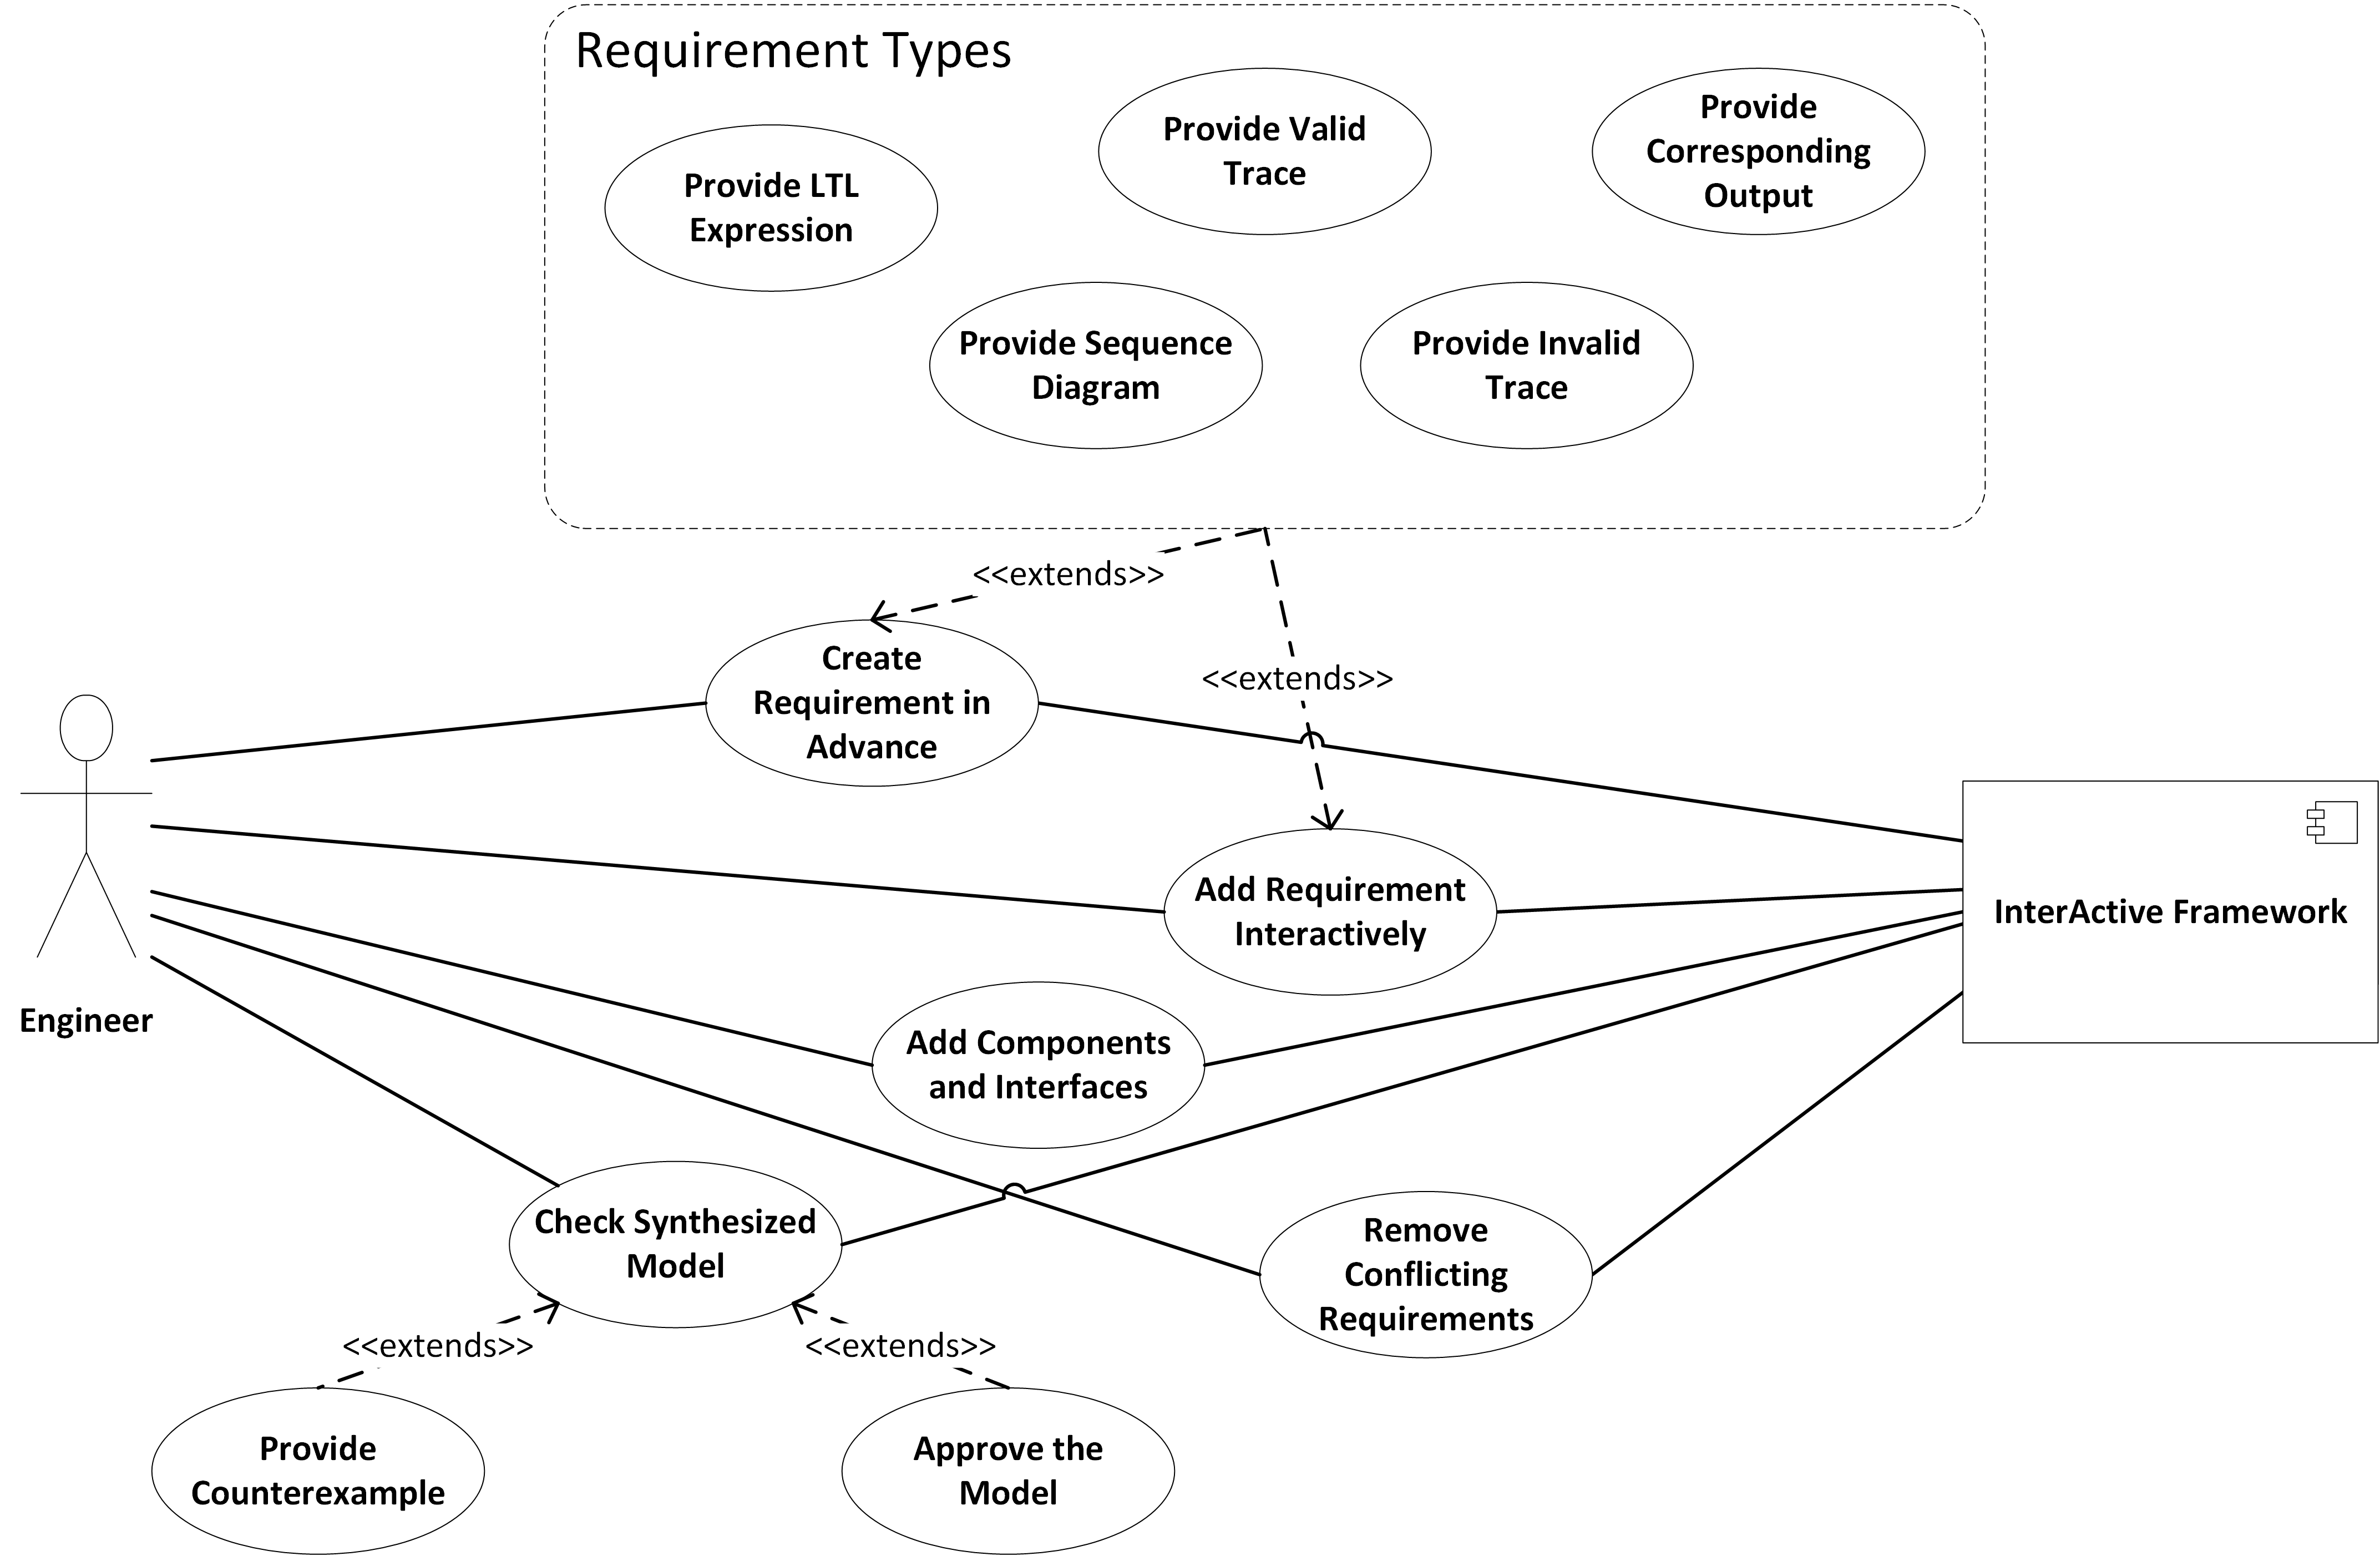
\includegraphics[width=150mm, keepaspectratio]{figures/methodology_interactiontypes.png}
	}
	\caption{Interaction types between the engineer and the ILE}
	\label{fig_methodology_interactiontypes}
\end{figure}

Our methodology is heavily based on the interaction of the user with the ILE. The different types of interacitons are summarized on Figure \ref{fig_methodology_interactiontypes} and are elaborated on in Subsection \ref{subs_reqtypes}. These interactions take place in a predefined order - the \textit{proposed workflow}, illustrated on Figure \ref{fig_methodology_workflow}. This workflow consists of two phases: first, an \textit{offline} one, and then an \textit{online} one, and ends with the serialization of the models. During the offline phase, the ILE offers little assistance, the designing engineer must determine the required details by other means. The interactive system design happens during the online phase. 

The individual steps in both the offline and the online phases have a predefined syntax with the corresponding, precisely defined semantics. Their common feature is the declarative way of describing the system components, which allows the engineer to focus solely on the expected behavior and acquire a minimal model exhibiting the specified functionality. The following subsections explain these steps in detail.

\begin{figure}[!ht] 
	\centering
	\fbox{
		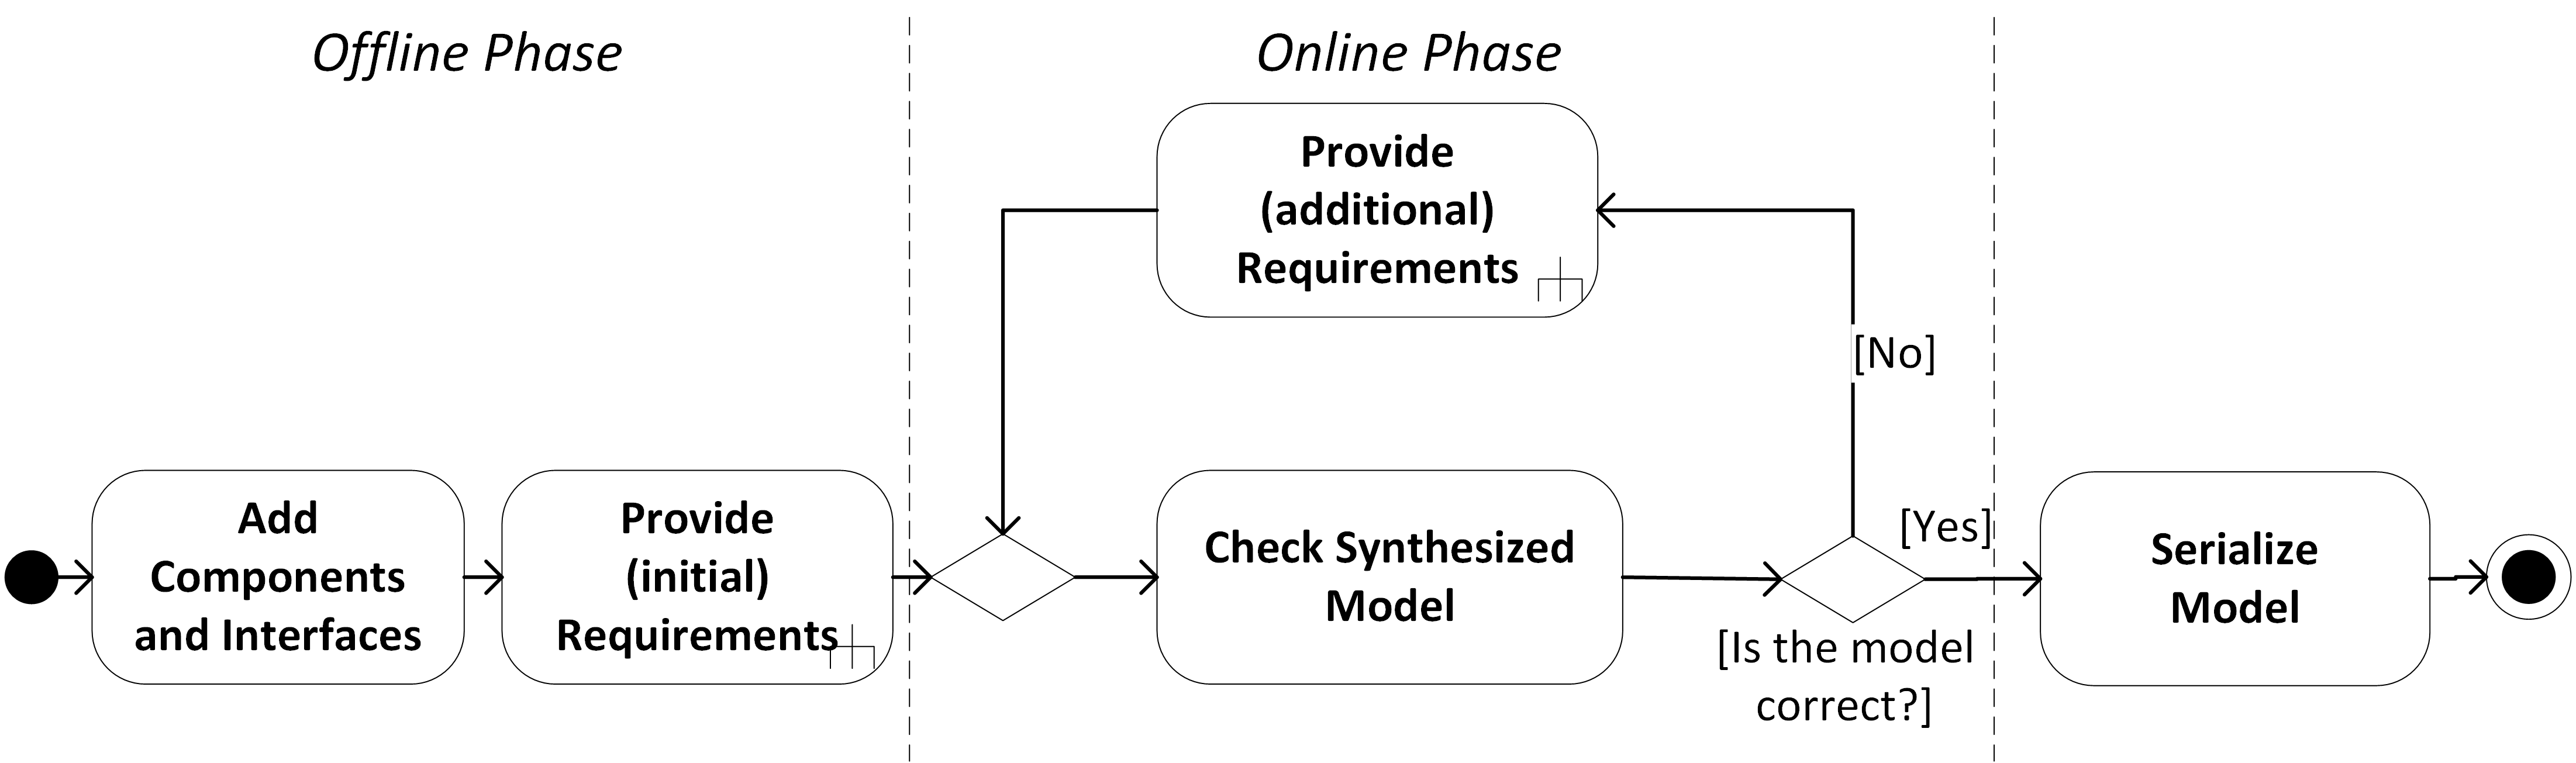
\includegraphics[width=150mm, keepaspectratio]{figures/methodology_workflow.png}
	}
	\caption{The Proposed Workflow}
	\label{fig_methodology_workflow}
\end{figure}
%TODO fork a komponenseknek

%---------------------------------------------------------------
\subsection{Component and Interface Definition} \label{subs_compdef}
%---------------------------------------------------------------
The first step of the workflow is the declaration of the system components. This happens in the offline phase, as the determination of the system components, their exact boundaries and interfaces is out of the scope of this work. Nonetheless, he engineer must provide the names of the system components, along with their interfaces - in other words their input- and output alphabets - before the workflow can proceed to the next step.

Users are encouraged to specify input and output characters qualified with interface names in the format 'Port.character', as this supplies the subsequent steps with essential information about the connections of the individual system components. For the sake of simplicity, this format is not necessarily used in the following examples.

The components are handled as independent systems in every other aspect. This results - among others - in the arbitrary ordering of the online behavior-learning phases, and the behavioral faults being limited to their components of origin (although this does not limit the propagation of errors through messages resulting from incorrect behavior).
The syntax of component and interface declarations is quite simple, as illustrated in Listing \ref{lst_compdef}.

\bigskip
\begin{lstlisting} [language=tex,caption=Example of a component declaration along with its interfaces,label=lst_compdef]
Components:
>component1 component2 component3
Input alphabet of component1:
>Input1.toggle Input2.interrupt
Output alphabet of component1: 
>Output1.red Output1.green Output1.blue
...
\end{lstlisting}

%---------------------------------------------------------------
\subsection{Requirement Types} \label{subs_reqtypes}
%---------------------------------------------------------------
During the workflow, the engineers can provide requirements in both the online and the offline phases. 

\begin{figure}[!ht] 
	\centering
	\fbox{
		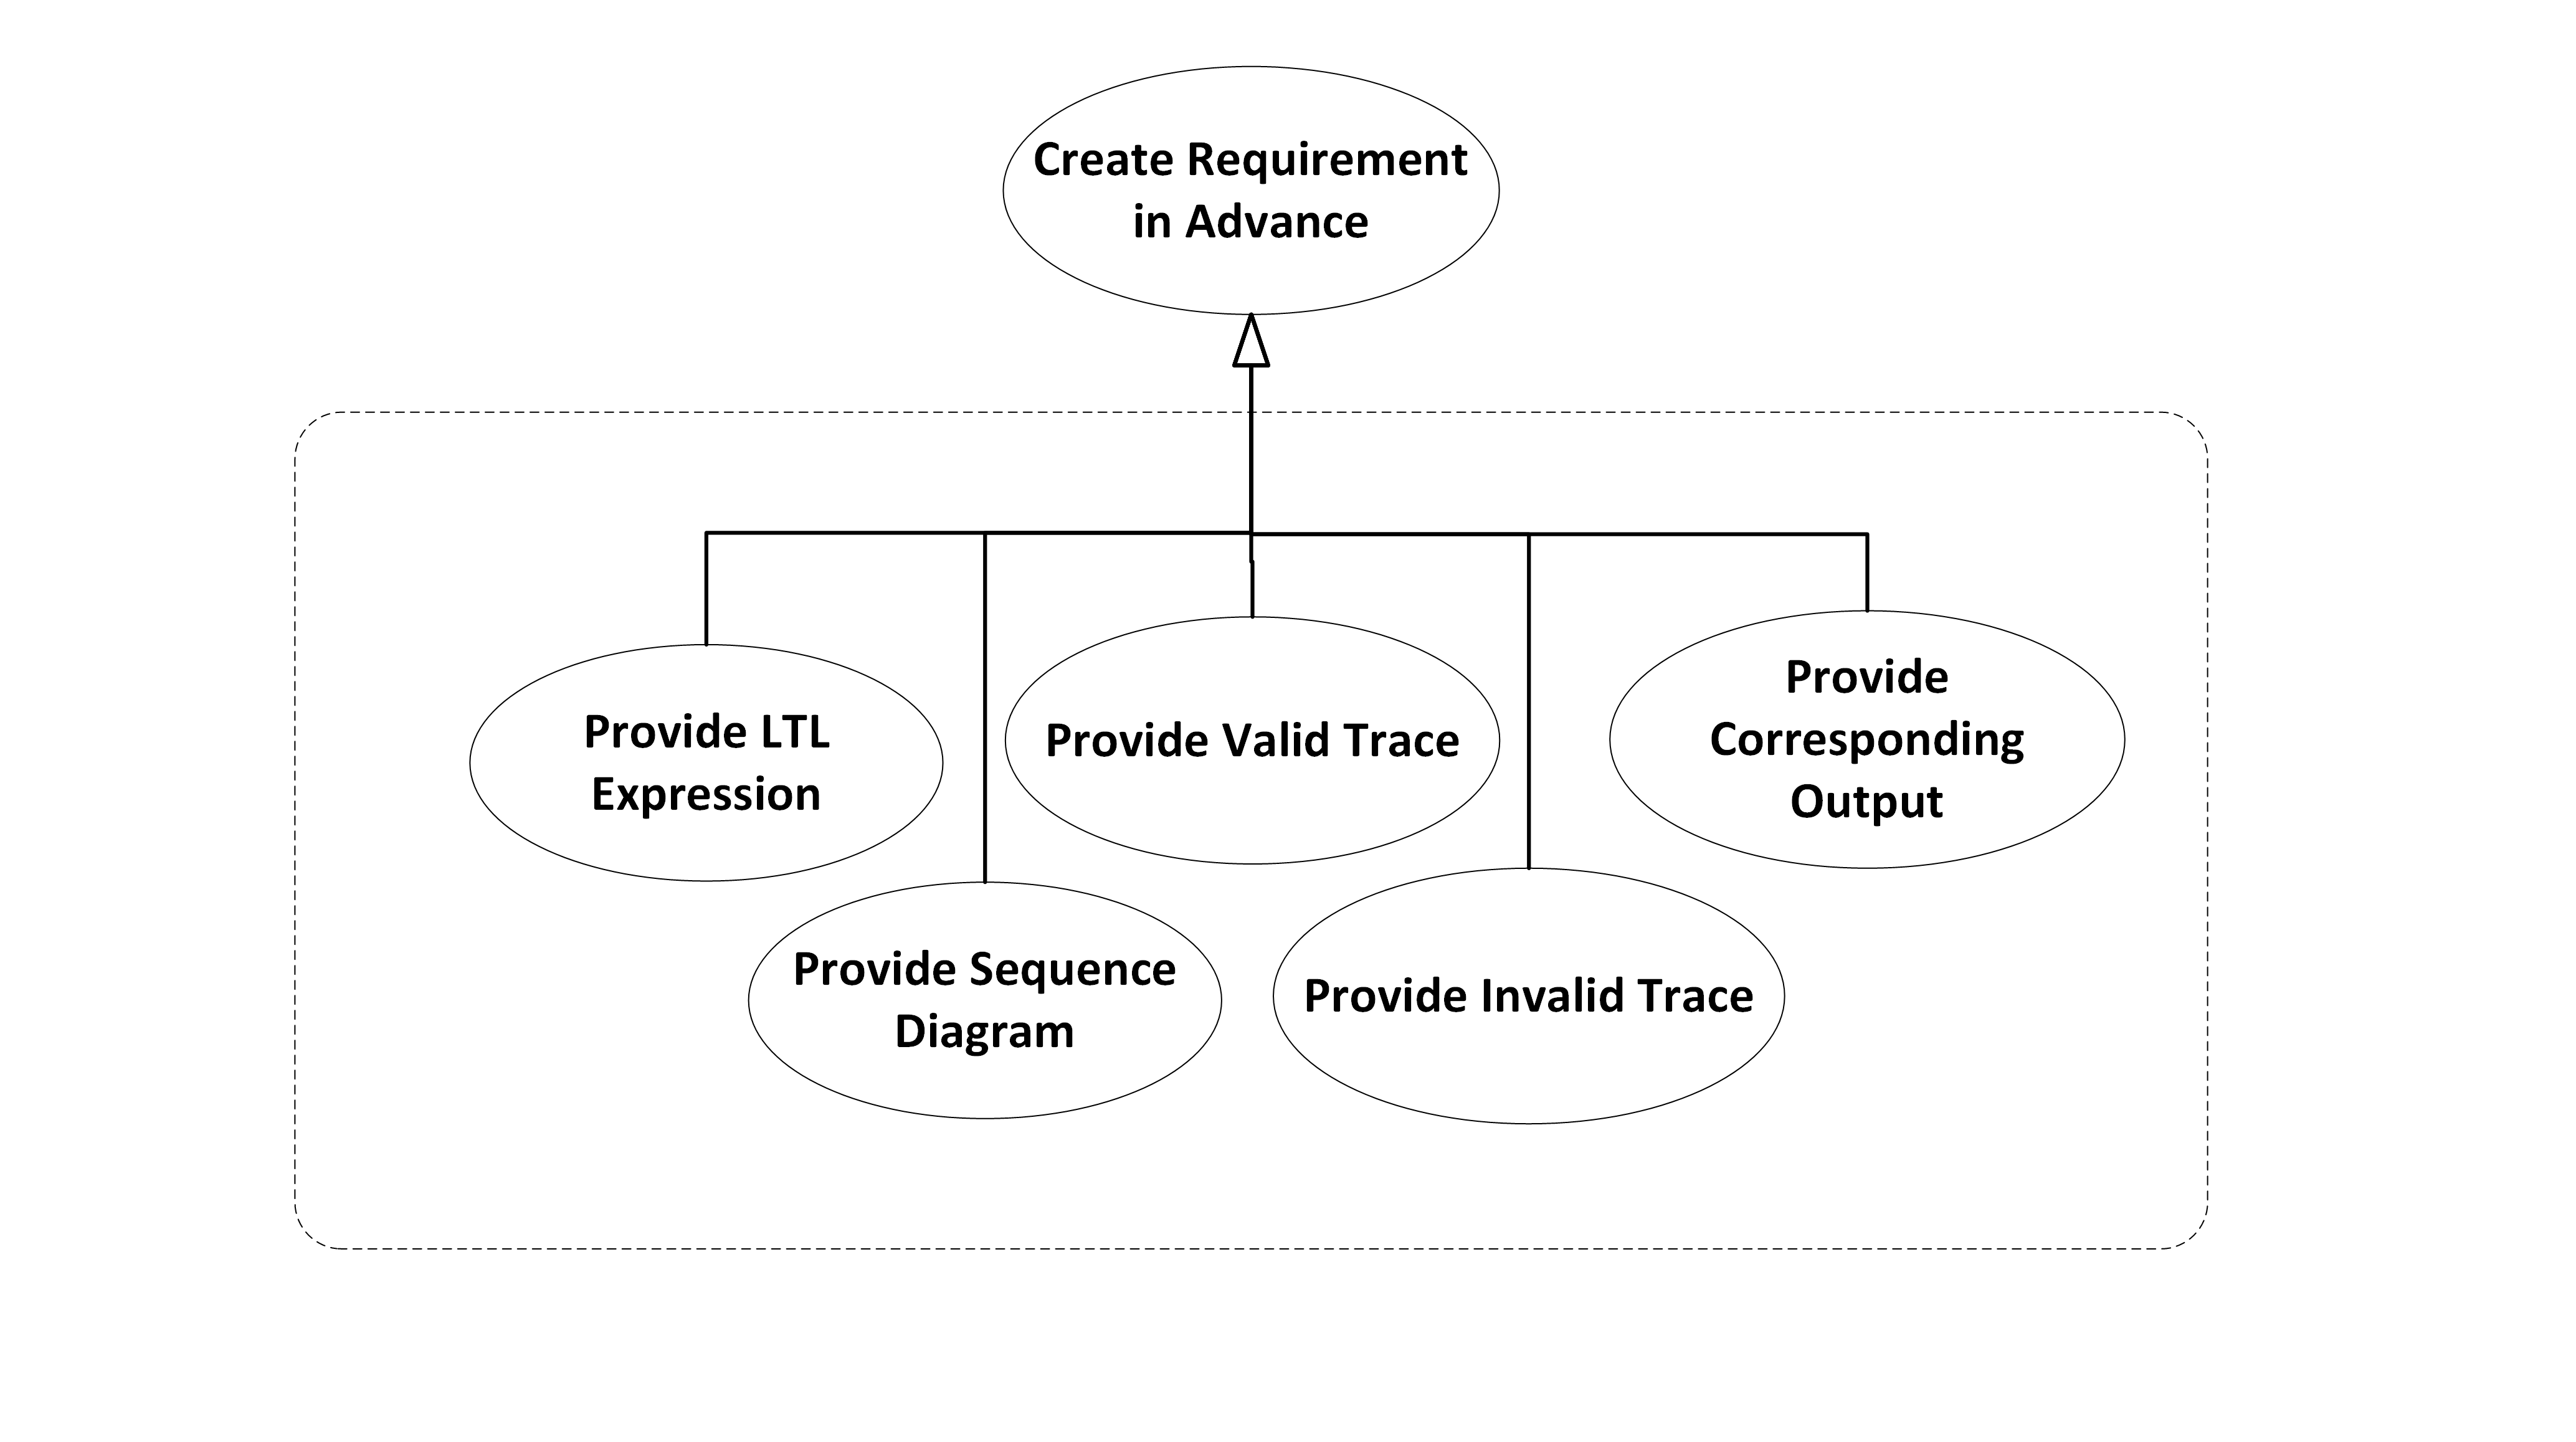
\includegraphics[width=150mm, keepaspectratio]{figures/methodology_requirementtypes.png}
	}
	\caption{The supported requirement types}
	\label{fig_requirementtypes}
\end{figure}

In the offline phase, this means that they add requirements they have formulated in advance. This is useful for more general requirements, with the scope of the whole component, conveniently formulated by program logic expressions, or long and complex traces.

In the online phase, adding requirements means answering the questions formulated by the algorithm about a yet unspecified behavior at a specific place in the trace currently being examined. This too can be answered through program logic - e.g. when the engineer realizes a general property during the model construction - but also through traces and through giving the corresponding output directly.

\textbf{Corresponding Output}
% TODO ref background: trace(-based)

This is the simplest way of specifying the behavior of the system, also containing the least amount of information among the different model types. To put simply, this means giving the output for a given input sequence, without any additional information. This supposedly answers the question of the ILE at \textit{one} given point, and that is the end of its scope.

Examples of corresponding output specification can be seen in Listing \ref{lst_iopair}.

\bigskip
\begin{lstlisting} [language=tex,caption=Examples of corresponding output specification,label=lst_iopair]
Offline: 
>input1 input2 input3 output

Online: 
>Output for [input1 input2 input3]:
>output3

(assuming input1/2/3 are from the input alphabet and output3 is from the output alphabet)
\end{lstlisting}

\textbf{Valid Trace}

Valid traces are a more complex form of specifying the corresponding output: it gives the corresponding output for any prefix of the contained input sequence. This might be useful, as usually the whole output sequence is taken into consideration when determining the output for some inputs. Thus, the ILE can obtain \textit{multiple} answers concerning the behaviors in question.

An example can be seen in Listing \ref{lst_validtrace}.

\bigskip
\begin{lstlisting} [language=tex,caption=Example of a valid trace,label=lst_validtrace]
Both offline and online:
>input1/output1 input2/output2 input3/output3

(assuming input1/2/3 are from the input alphabet and output1/2/3 are from the output alphabet) 
\end{lstlisting}

\textbf{Sequence Diagram}
%TODO ref backgr UML

UML-like sequence diagrams - the ones introduced in [TODO ref backgr] - are an even more complex form of trace-based models, as they can contain several traces, due to them having various combined fragments for branching the behavior - like \textit{alt} and \textit{opt} - and for referencing behaviors specified elsewhere - like \textit{ref}.

Sequence diagrams can also be used to model infinite behavior, which results in containing plenty of information, which in turn results in possibly answering \textit{several} questions formulated by the ILE.

%TODO
An example for the application of sequence diagrams can be seen on [TODO insert example]

It is important to note, that the specification and integration of sequence diagrams into this framework is not yet complete. 

\textbf{Trace to Exclude}

Invalid traces are similar to valid traces, with the difference that the contained behavior must not appear in the resulting model. They are most useful for small output alphabets, or when the range of possible behaviors is otherwise contained - e.g. through program logic expressions or several other excluded traces.

They can also be used to formulate requirements when the determination of the correct behavior does not directly follow from them: when specifying the behavior in question, the ILE will signal any conflicting requirements for the examined input sequences and require the user to remove one - thus facilitating the enforcement of these requirements too.

An example for invalid traces can be seen in Listing \ref{lst_invalidtrace}.

\bigskip
\begin{lstlisting} [language=tex,caption=Example of a trace to exclude,label=lst_invalidtrace]
Both offline and online:
>input4/output4 input5/output5

(assuming input4/5 are from the input alphabet and output4/5 are from the output alphabet) 
\end{lstlisting}

\textbf{LTL Expression}
%TODO ref backgr LTL
%TODO ref backgr LTS

LTL expressions are a highly complex type of program logic-based requirement specification: they can be used to formulate propositional logic expressions with temporal connectives over \textit{paths} of a \textit{base model}, as described in [TODO ref backgr]. 

For our application, we introduce our own LTL expression language with its own syntax and semantics - although attempting to keep it similar to other generally known variants, especially that of SPOT [TODO cite]. The full syntax of the LTL expressions - also determining the operator precedence - can be seen in Listing \ref{lst_ltlfullsyntax}.

The base model of the LTL expressions is the LTS [TODO ref backgr] interpretation of the component under learning. This means, that the set of atomic propositions that can be used in these expressions are the possible labels of the transitions, which are the elements of the input and the output alphabets of the component. The model synthesis takes place assuming event semantics - exactly one input and one output event happening at any given time. For this reason, we also introduced these semantics to the LTL expressions: the conjunction of exactly one input and one output character must hold at any given point in time for it to be considered correct - and every other character must be negated at the same point. This also entails, that given another character not explicitly negated at that point, it is assumed to be automatically negated, and in the case that no proposition is declared explicitly to hold, it is assumed that either one of the non-explicitly negated characters hold. 

The semantics of the supported temporal connectives, and other aspects of the LTL semantics in general, are similar to those described in [TODO ref backgr] %TODO

Examples for a valid LTL expressions can be seen in Listing \ref{lst_ltlex}.

\bigskip
\begin{lstlisting} [language=tex,caption=Examples of LTL expressions,label=lst_ltlex]
Assuming Control.interrupt and toggle are from the input alphabet and blinkingYellow is from the output alphabet, both offline and online:
>F(interrupt -> X(G(toggle) -> G(blinkingYellow)))

Assuming the output alphabet also contains red, yellow and green, it is equivalent to:
>F(interrupt&!toggle -> X(G(toggle&!interrupt) -> G(blinkingYellow&!red&!yellow&!green)))
\end{lstlisting}

It is important to note, that the specification of our LTL variant is not yet complete: for the compactness of requirement specifications it would make sense to integrate additional well-known boolean operators - like XOR (exclusive-or) - and temportal connectives - such as WB (weak-before) and R (release) - into the language. 

%---------------------------------------------------------------
\subsection{Conflicting Requirements} \label{subs_conf}
%---------------------------------------------------------------
The requirements the designing engineer provides the ILE with may easily be conflicting, especially in case of LTL expressions and invalid traces - that describe possibly infinite sets of behaviors. For this reason, it is essential for the system to provide some kind of conflict handling within the practical boundaries of the available resources. 

This problem is a difficult and resource intensive task for algorithmic reasons elaborated later. Consequently, the ILE only guarantees to handle the conflict, when it also interferes with the model synthesis, in which case, the user is asked to remove one of the conflicting models, before the analysis of the behavior can proceed.

\begin{figure}[!ht] 
	\centering
	%\fbox{
		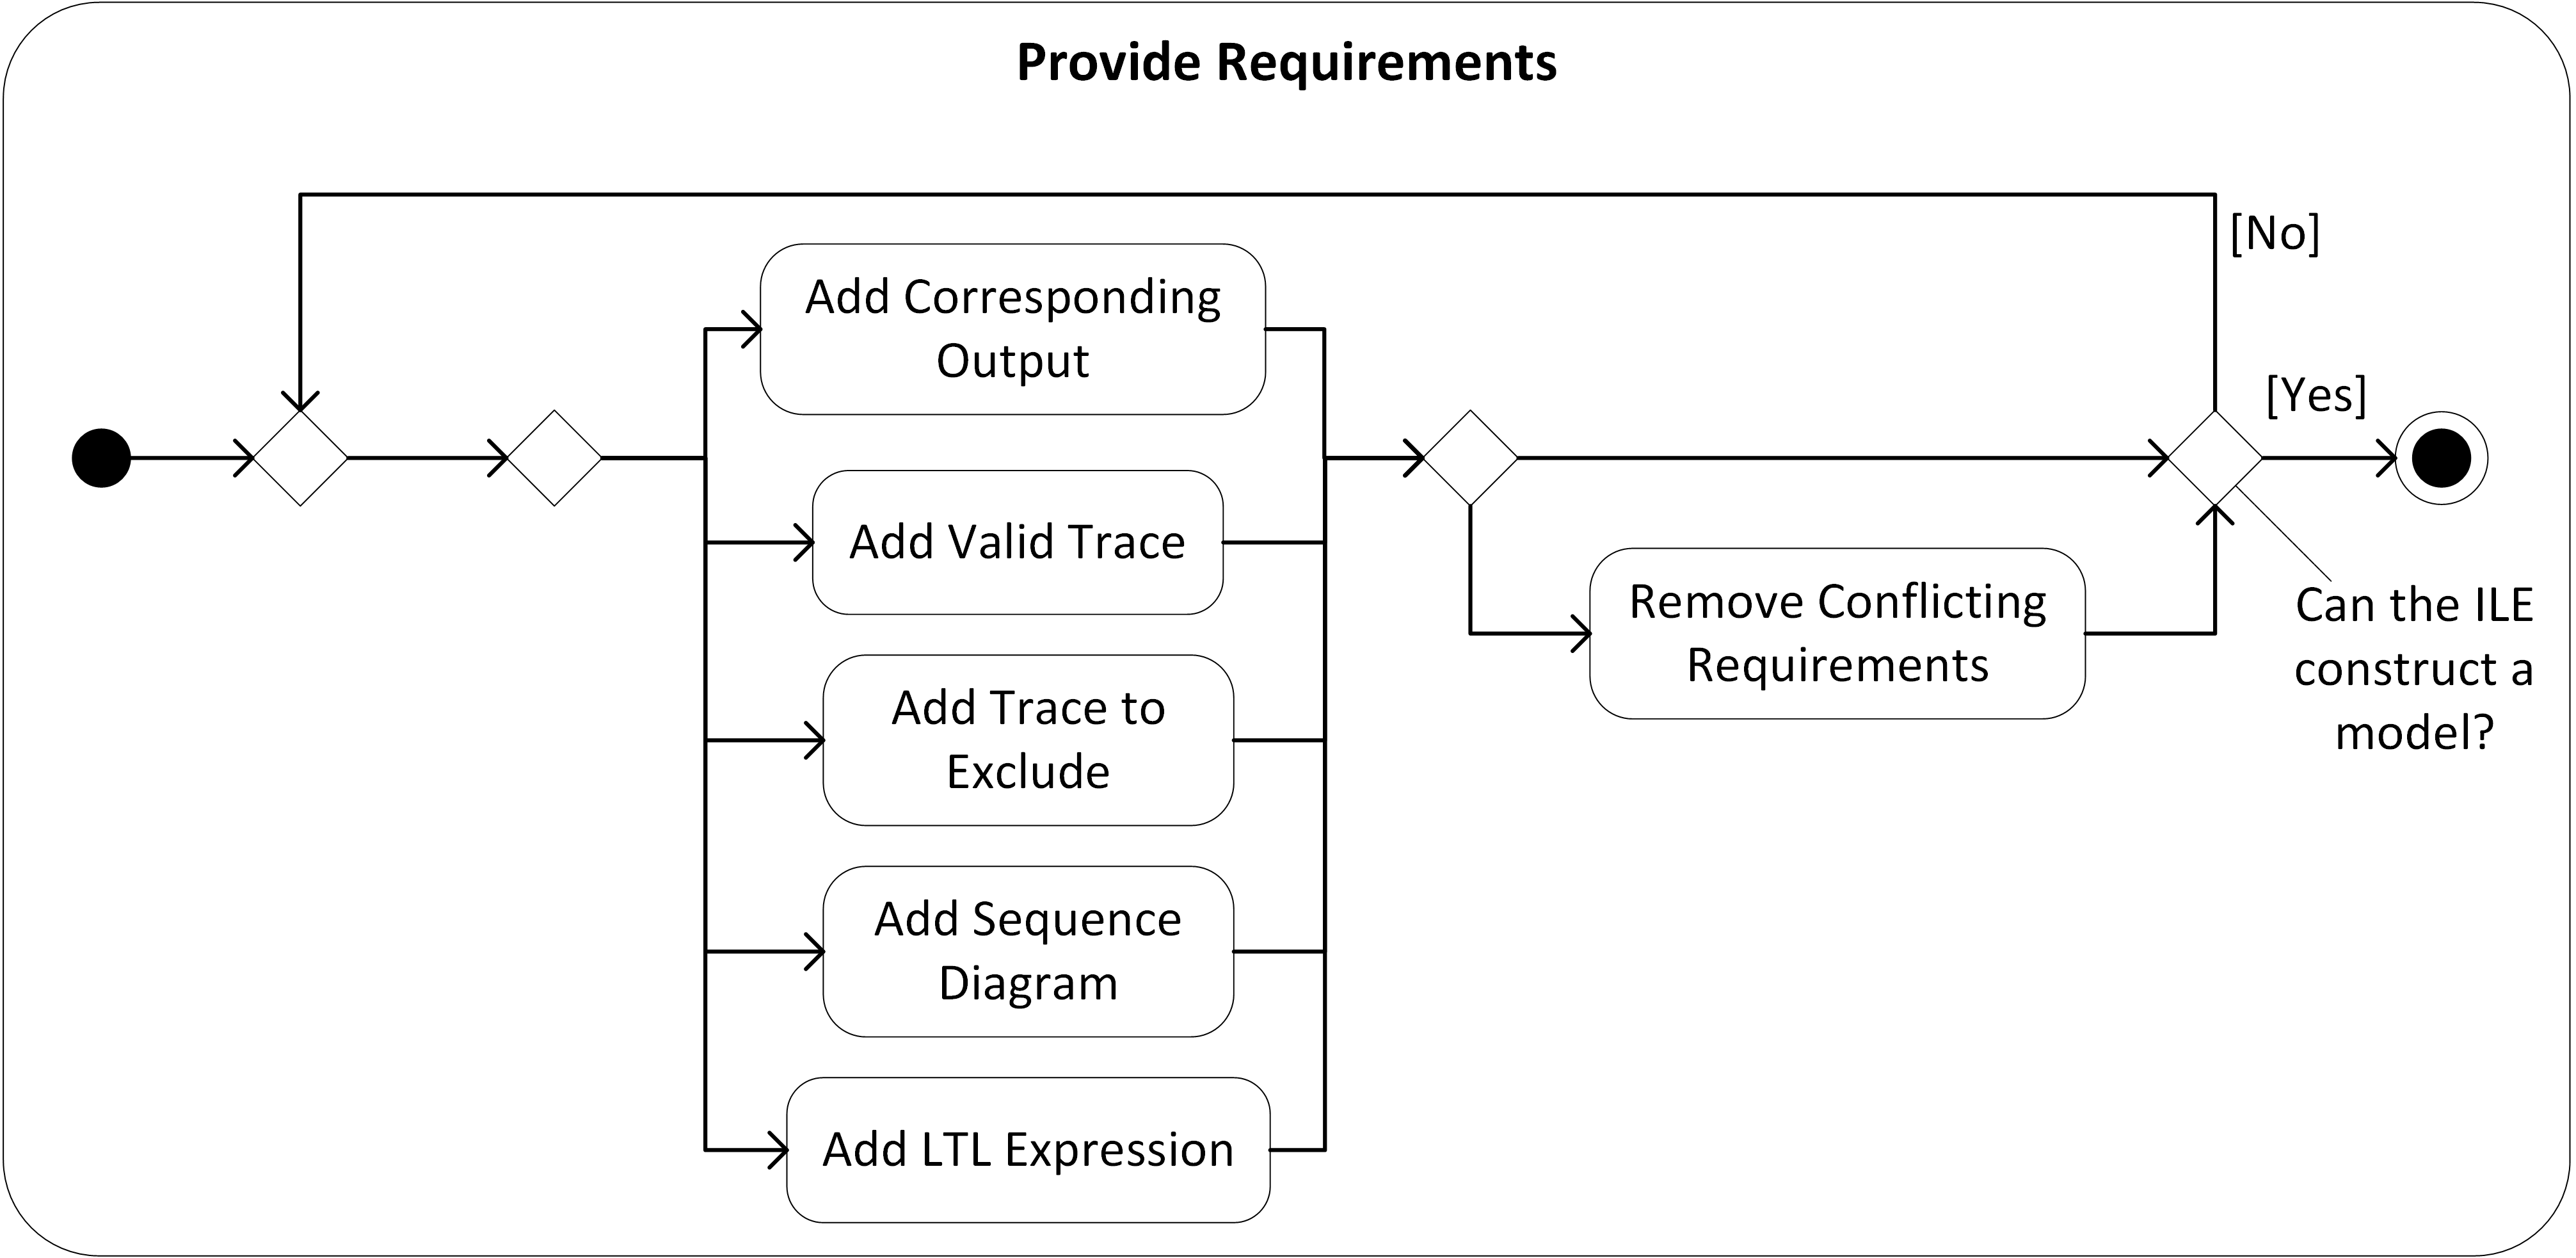
\includegraphics[width=130mm, keepaspectratio]{figures/methodology_providerequirementsworkflow.png}
	%}
	\caption{The process of adding a requirement}
	\label{fig_providerequirementsworkflow}
\end{figure}


As conflicts only become apparent during the online phase of the workflow, the conflict handling is only present there. However, conflicts that were introduced earlier are also discovered and resolved in that phase. An example of a requirement conflict handling can be seen in Listing \ref{lst_conflicthandling}.

\bigskip
\begin{minipage}{\linewidth}
\begin{lstlisting} [language=tex,caption=Example of a requirement conflict handling,label=lst_conflicthandling]
	TODO EXAMPLE
	TODO EXAMPLE
\end{lstlisting}%TODO
\end{minipage}

%---------------------------------------------------------------
\subsection{Checking the Correctness of the Synthesized Model} \label{subs_eq}
%---------------------------------------------------------------
During the online phase, whenever ILE assumes that it has gathered enough information to construct a model for the given component, the engineer if offered with a possible model representing the current state of the model synthesis - the equivalent of an equivalence query in automaton learning algorithms. This model can either be approved, or a counterexample is required from the user, where the model does not meet the - not yet specified - requirements.

The proposed equivalence model is a deterministic automaton, which, based on the information provided by the user, can be incomplete in multiple ways. The behavior of the proposed model can differ from the learned systems because of lacking information, in which case the user (acting as the equivalence oracle of the learning) needs to provide the separating behavior. Another reason for incompleteness is newly discovered states, the behavior of which is unknown based on their input signatures. This case prompts the user to evaluate the validity of state separation and is required to provide the lacking information. If, for some reason the hypothesized behavior is contradicting that of the imagined system (by the users oversight in providing requirements), the actual, conflicting requirement can be provided to guide the learning algorithm through the process described in Subsection \ref{subs_conf}.

If the model is accepted, the workflow can attempt to proceed to the next step - the serialization of the model. If a counterexample is provided, the online phase resumes and the system design continues until the next possible model is reached.

Examples of models offered in equivalence queries can be seen on Figure \ref{fig_methodology_eqex}.

\begin{figure}[!ht] 
	\centering
	\fbox{
		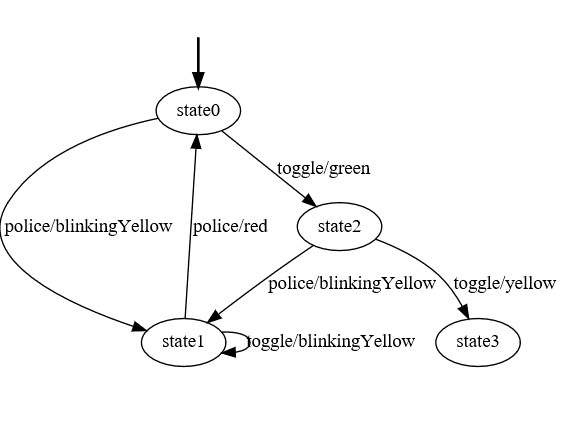
\includegraphics[height=50mm, keepaspectratio]{figures/methodology_eqex1.png}
	}
	\fbox{
		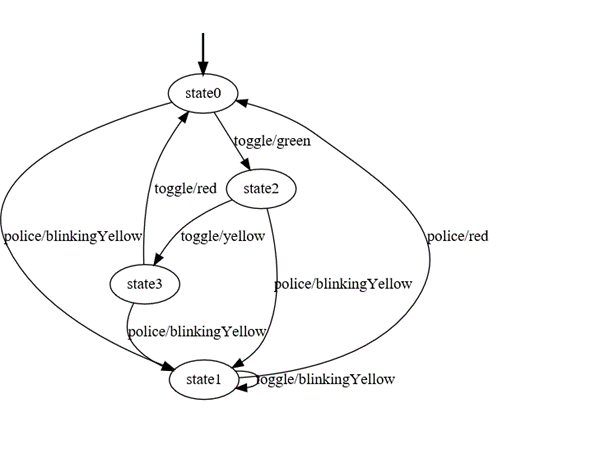
\includegraphics[height=50mm, keepaspectratio]{figures/methodology_eqex2.png}
	}
	\caption{Equivalence query for an incomplete model (\textit{left}) and the final model (\textit{right})}
	\label{fig_methodology_eqex}
\end{figure}

%---------------------------------------------------------------
\subsection{The Resulting System Model} \label{subs_resultingmodel}
%---------------------------------------------------------------
When each of the component models declared during the first step of the workflow are completed, the resulting system model can be serialized and handed over to the engineer for further extensions or to use it for any of its possible applications. This serialization can happen in various formalisms.

%TODO ref 
One such possible formalism is the serialization to a Gamma statechart, introduced in [TODO ref backgr]. Gamma statecharts are high-level state-based models, to which every functionality offered by the Gamma Statechart Composition Framework can be applied. Our framework offers full-scale Gamma serialization: when choosing this formalism, a whole project will be created, along with interface definitions, component definitions - for each of the previously declared components, with the synthesized behavior - and a composite system definition, connecting the components based on the names of their interfaces.

%TODO ref
Another possibility is the serialization to the Mealy machine formalism of the framework - as presented when checking the correctness of the model. This results in a lower-level set of independent models, with a completely different set of applications.

%TODO interface definitions vs component diagram
[TODO figure comes here: [comps\&interfaces | resulting structure]]
\clearpage
%----------------------------------------------------------------------------
\section{Overview of the Architecture} \label{sec_architecture}
%----------------------------------------------------------------------------

The architecture of the ILE consists of two main components: the automata learning algorithm - which is responsible for the model synthesis procedure, thus the course of the learning - and the interactive oracle - investigating the membership of the given input sequences in the languages of the models given by the user on one side and interacting with the user on the other. This architecture is depicted on Figure \ref{fig_architcture_ileoverview}. The following subsections elaborate on the connections and details of these components. 

\begin{figure}[!ht] 
	\centering
	\fbox{
		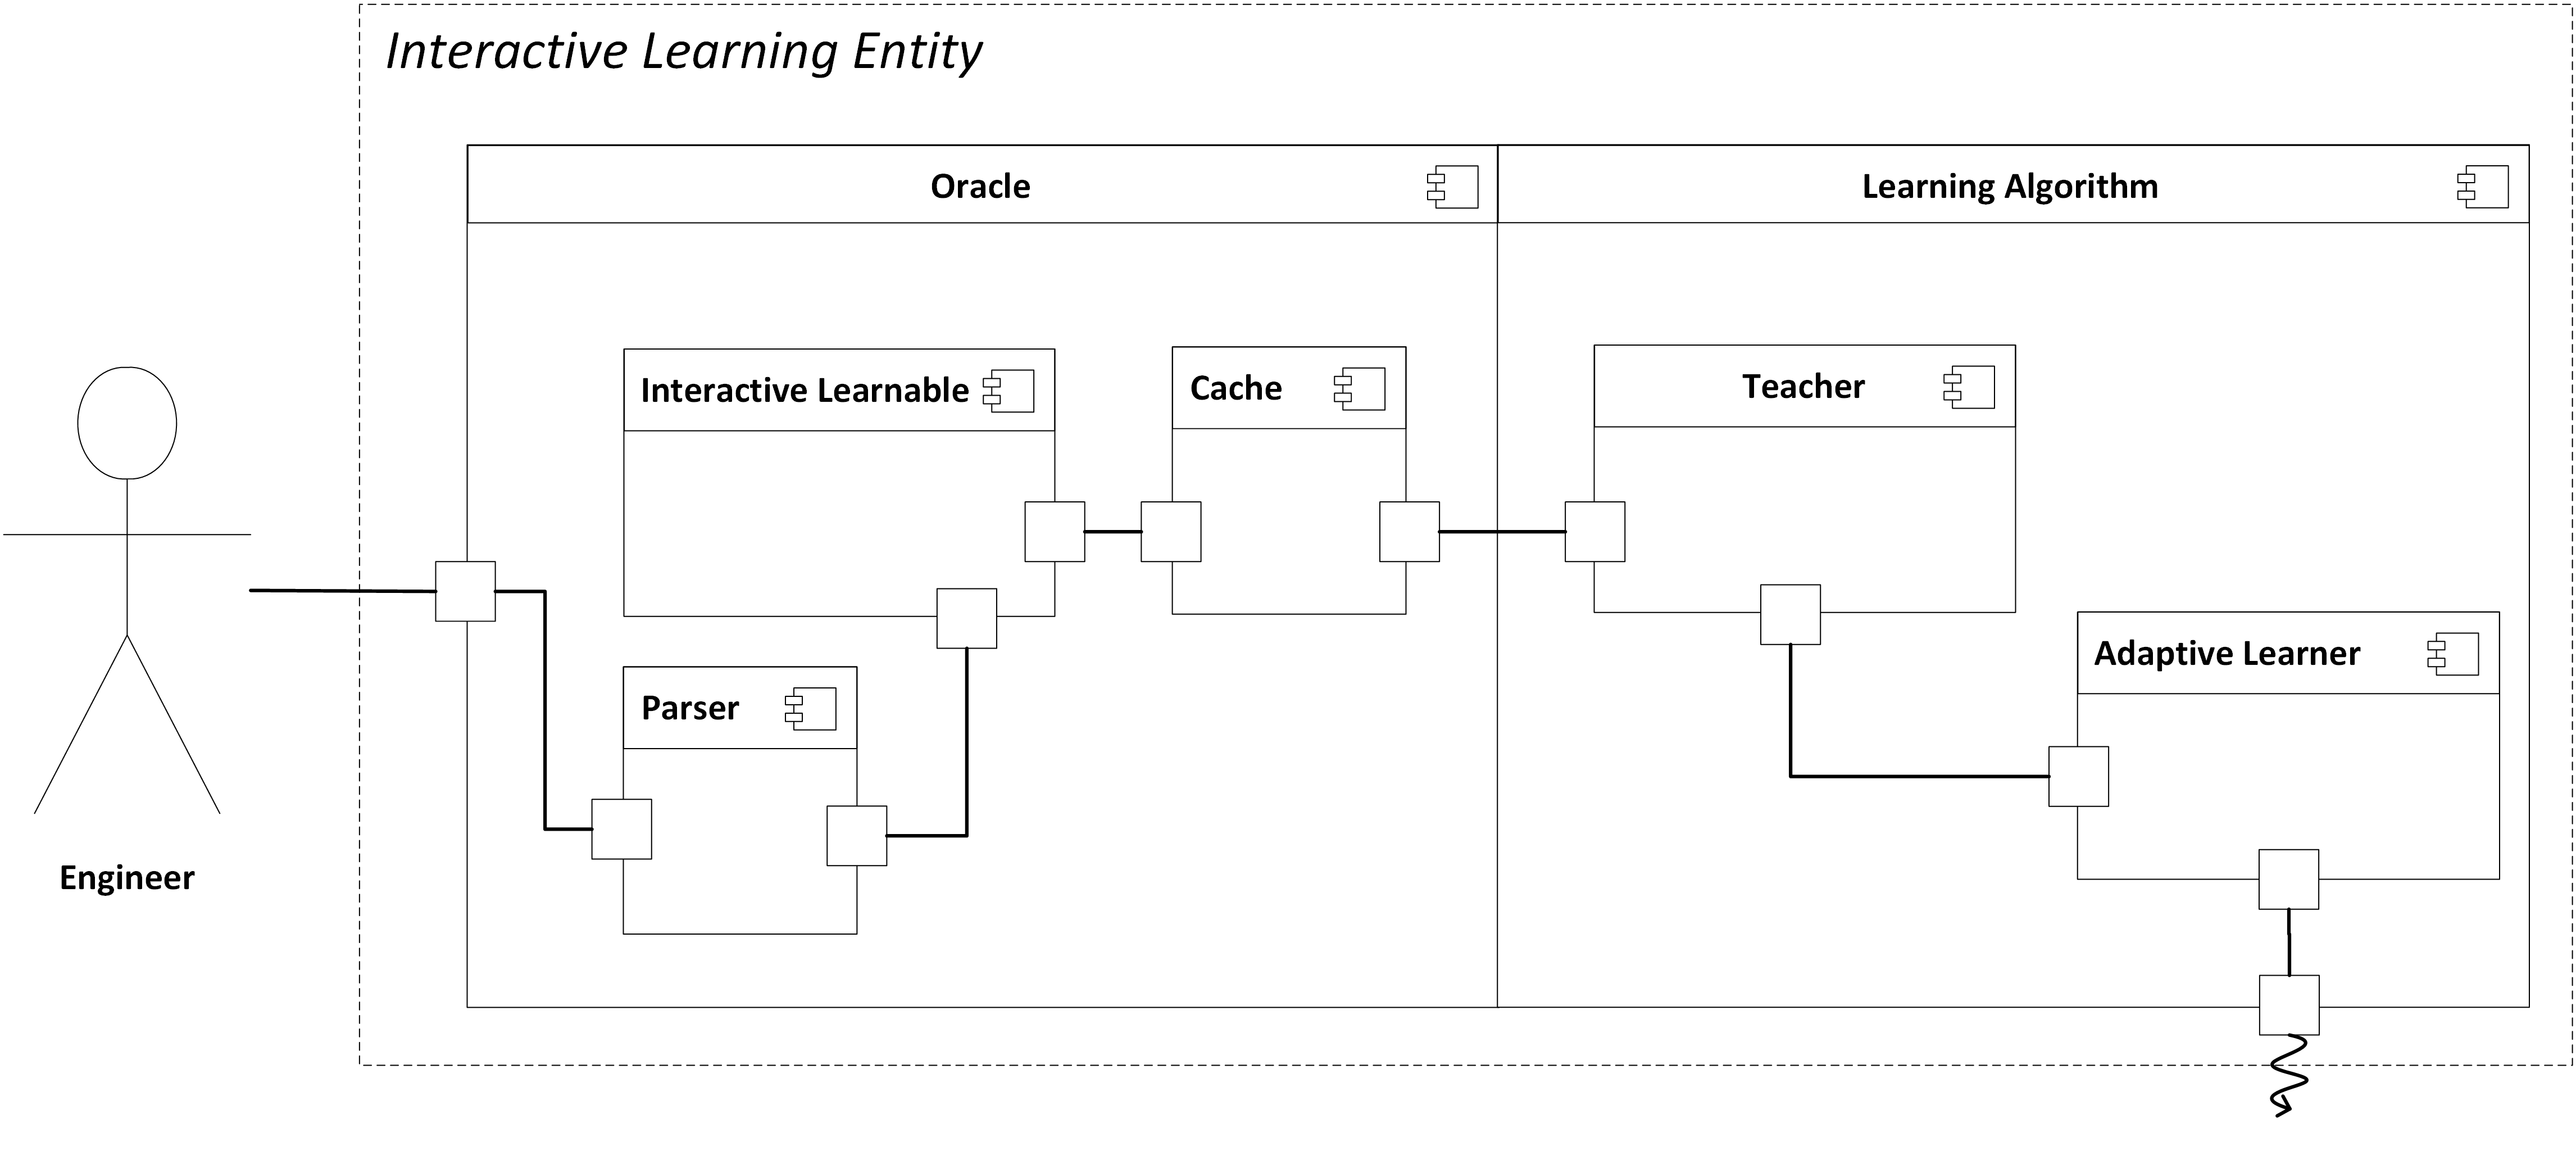
\includegraphics[width=150mm, keepaspectratio]{figures/architecture_ileoverview.png}
	}
	\caption{High-level architecture of the components of the ILE} 
	\label{fig_architcture_ileoverview}
\end{figure}

%---------------------------------------------------------------
\subsection{Automata Learning in the Framework} \label{subs_automatalearningintheframework}
%---------------------------------------------------------------
(learner <-> teacher)
%TODO (the teacher delegates the questions to the interactive learnable, which in turn delegates to the user ...)
%---------------------------------------------------------------
\subsection{The Underlying Algorithm} \label{subs_dhcintheframework}
%---------------------------------------------------------------
(dhc variant)
%TODO
%---------------------------------------------------------------
\subsection{Automata Minimization} \label{subs_minimizationintheframework}
%---------------------------------------------------------------
(per round vs per learning)
%TODO
%---------------------------------------------------------------
\subsection{Caching} \label{subs_cachingintheframework}
%---------------------------------------------------------------
(memoizing learnable)
%TODO: az oracle kérdezése költséges, így minél kevesebbszer akarjuk kérdezni
%---------------------------------------------------------------
\subsection{The Cost of Exploration (Command Handling)} \label{subs_commandhandling}
%---------------------------------------------------------------
(egyéb cím ötletek: a könnyen felfedezhető részek nyilvántartása, controlling the design space exploration, design space optimization, knowing what is unknown, reducing the cost of exploration, controlling design space partitions, abstract space partitioning, concept class)
%TODO: a költség az, hogy hányszor kérdezzük a usert, ezt akarjuk csökkenteni. Így nyilvántartjuk, hogy merre tudunk még információt kinyerni a már meglévő modellekből, csak azután megyünk a felhasználóhoz.
\begin{figure}[!ht] 
	\centering
	%\fbox{
	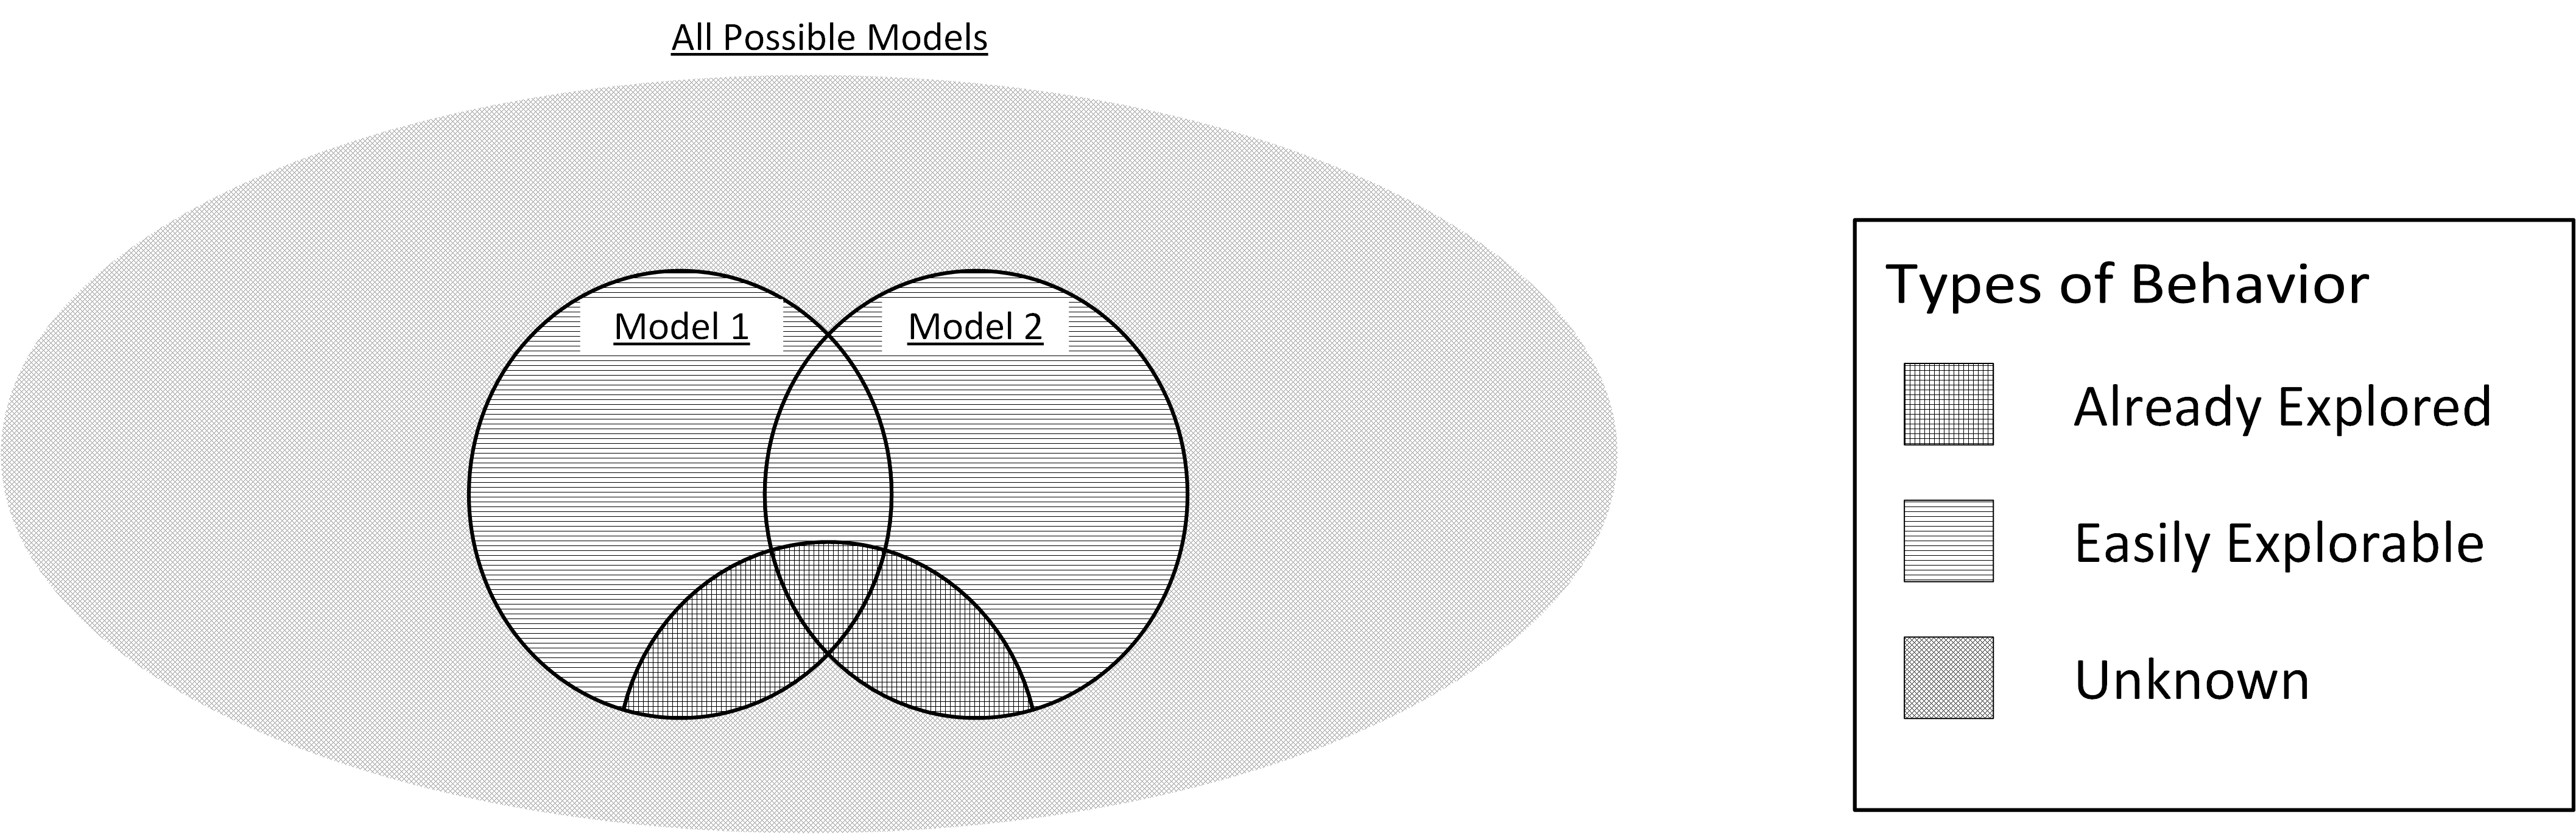
\includegraphics[width=100mm, keepaspectratio]{figures/architecture_commandhandling.png}
	%}
	\caption{Types of behavior during the learning process} 
	\label{fig_architcture_commandhandling}
\end{figure}

%---------------------------------------------------------------
\subsection{Interactive Learnable} \label{subs_oracle}
%---------------------------------------------------------------
(hogyan foglalja össze a partial modeleket)
%TODO 
\begin{figure}[!ht] 
	\centering
	%\fbox{
		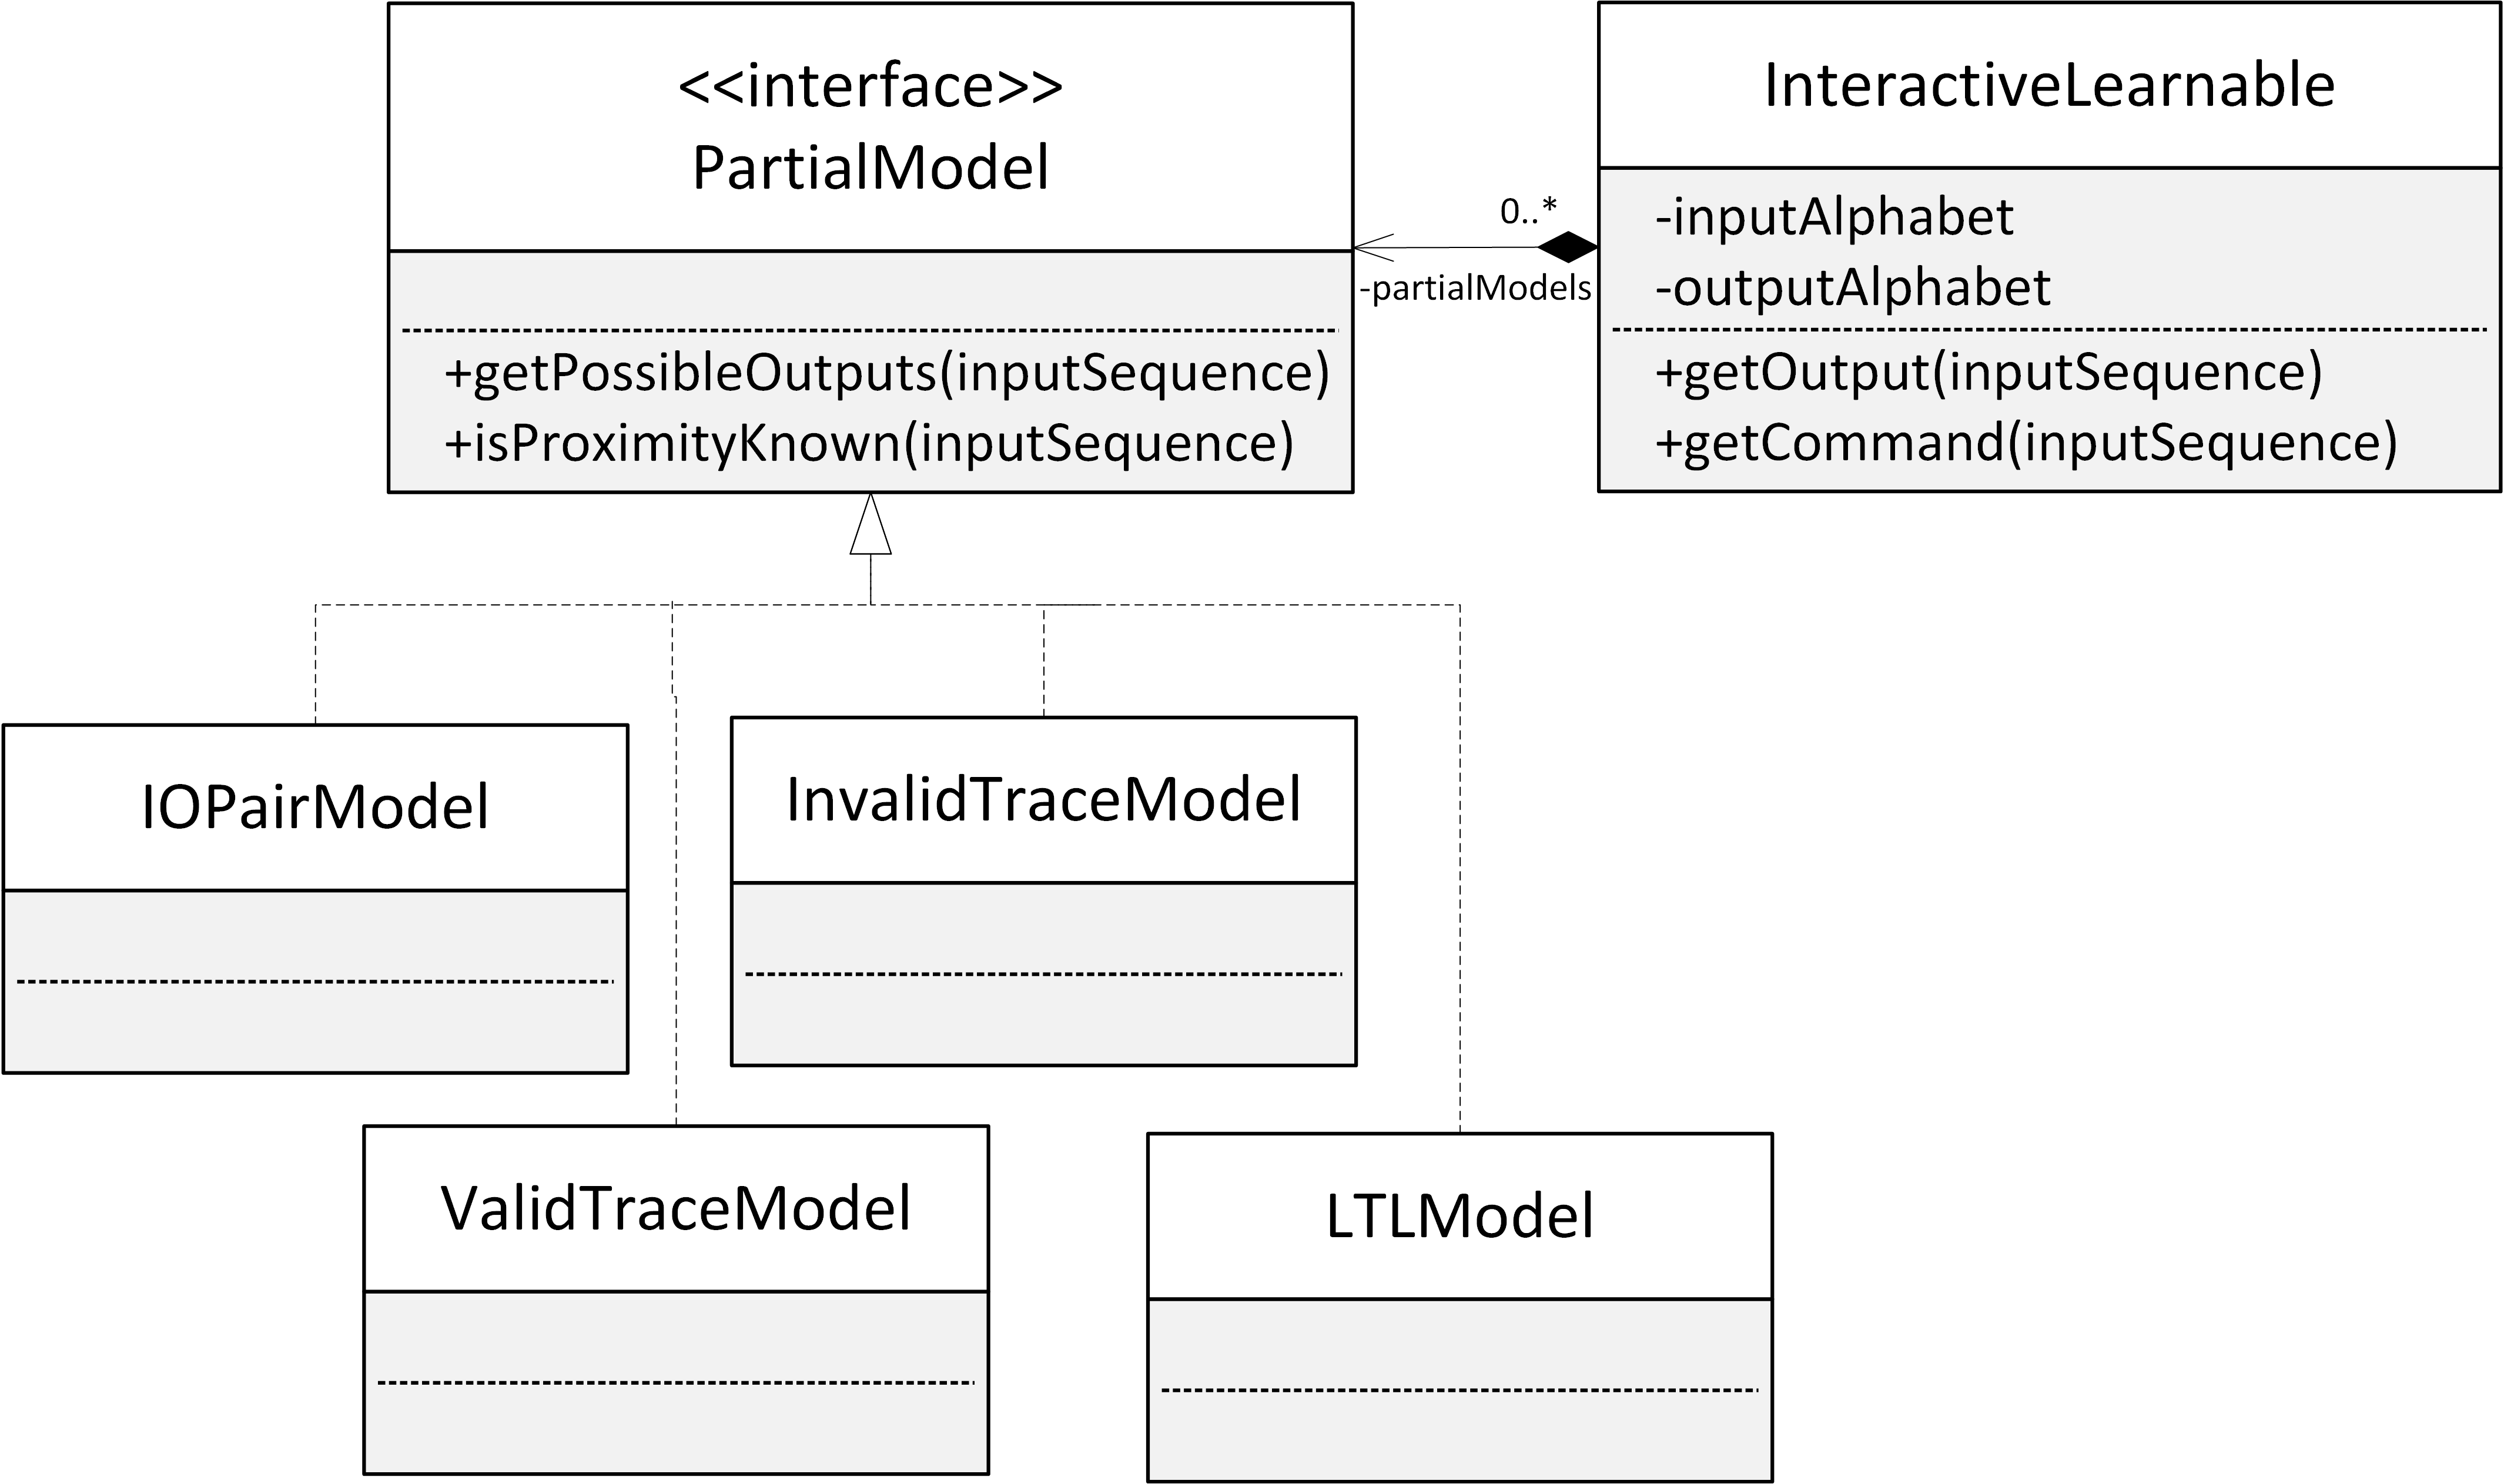
\includegraphics[width=150mm, keepaspectratio]{figures/architecture_interactivelearnable.png}
	%}
	\caption{Architecture of the interactive learnable component} 
	\label{fig_architcture_interactivelearnable}
\end{figure}

%---------------------------------------------------------------
\subsection{Trace-Based Models} \label{subs_traceintheframework}
%---------------------------------------------------------------
%TODO 
(hogyan működnek)
%---------------------------------------------------------------
\subsection{LTL Models} \label{subs_ltlintheframework}
%---------------------------------------------------------------
%TODO 
(hogyan lesznek használhatóak és hogyan működnek)
%----------------------------------------------------------------------------
\chapter{Implementation}
%----------------------------------------------------------------------------

%TODO: bevezetes
%----------------------------------------------------------------------------
\section{Tooling} \label{sec_tooling}
%----------------------------------------------------------------------------
%TODO: random bevezeto szoveg

%----------------------------------------------------------------------------
\subsection{Eclipse Environment} \label{subsec_emf}
%----------------------------------------------------------------------------
Eclipse is a popular, open-source integrated development environment (IDE). It is mainly used for Java-related application development, but also supports several other programming languages. It consists of a base workspace and an extensible plug-in system. Using this plug-in system, the develpment environment is easily customizable for different purposes, such as programming in different programming lanugages, modeling (using the Gamma Framework or Yakindu), or testing.

\textbf{Eclipse Modeling Framework}

The Eclipse Modeling Framework is an Eclipse-based modeling framework and code generation facility. It defines its own structured data model -- called Ecore -- for describing models and providing runtime support for the models. Models are defined using the XML Metadata Interchange (XMI) format, which is supported by various Eclipse plugins developed specifically for this purpose, as EMF is fully integrated into the Eclipse platform. It provides an environment to numerous technologies, including server solutions, persistence frameworks, UI and transformation frameworks.

%----------------------------------------------------------------------------
\subsection{Xtext Framework} \label{subsec_xtext}
%----------------------------------------------------------------------------
Xtext is an open-source framework for developing (mostly) domain-specific languages (DSLs). It has its own syntax for the definition of textual languages, resembling a context-free grammar extended with mappings to the in-memory representations. Unlike standard parser generators, it generates not only a parser, but also the abstract syntax tree (AST) of the grammar, and also support several other features, such as validation rules and editing support. This is because Xtext is based on the EMF project -- the metamodels of the defined languages are Ecore models --, and it is integrated into the Eclipse environment.

\textbf{Xtend}

Xtend is a general-purpose, high-level programming language based on Java. It is statically typed, object-oriented and uses the type system of Java. Xtend programs are compiled to Java code, thus allowing seamless integration with existing Java libraries. It provides numerous convenient extensions to Java, such as dispatch methods, type inference, operator overloading and extension methods.

%----------------------------------------------------------------------------
\subsection{Sirius} \label{subsec_sirius}
%----------------------------------------------------------------------------
Sirius is an open-source project for developing graphical modeling languages. It is integrated into the Eclipse environment, enabing the specification of viewpoints for EMF models, thus the creation of graphical views. In a Sirius workbench (editor), the elements of the viewpoint specification models are mapped to individual EMF model elements, thus allowing their graphical interpretation and editing. The whole viewpoint definition procedure is declarative, using OCL \cite{OCLStandard} (or Acceleo Query Language, AQL) expressions for the traversal of the diagram elements when needed.

Sirius supports various representation types. Traditional Sirius diagrams consist mainly of nodes and edges between nodes, suitable for models in which the position of the diagram elements carries no meaning - like several structural modeling languages. It also supports table and tree representations, and also \textit{sequence diagrams} for modeling behavior - in which the position on the diagram is also part of the semantics.

%----------------------------------------------------------------------------
\subsection{Owl} \label{subsec_owl}
%----------------------------------------------------------------------------

Owl \cite{Owl} is a tool collection for $\omega$-words, $\omega$-automata and linear temporal logic. It provides several algorithms for automata and LTL, supporting - among others - LTL expression parsing and simplification, reading and writing $\omega$-automata using the HOA format \cite{HOAFormat}, translation of LTL formula to $\omega$-automata with several possible acceptance conditions, and operations over $\omega$-automata, such as product, SCC decomposition emptiness checks and acceptance-condition transformations.

Through providing these algorithms, the library supports easy development and fast prototyping in the area of LTL and automata, thus also enabling rapid concept validation.

%----------------------------------------------------------------------------
\subsection{Automata Learning Framework} \label{subsec_automatonlearning}
%----------------------------------------------------------------------------
In order to give a foundation to the implementation described in this thesis, a previously created automata learning framework TODO: ref BSC] was extended upon. Since the framework was implemented using the Java programming language, the high-level view seen in Figure \ref{fig_automatalearning_packages} is represented as an UML class diagram of the packages and the relations between them, essentially being an overview of the modularization of the framework. 


\smallskip

The \textit{Learnable} package contains the input formalisms, and the \textit{Hypothesis} package contains the output formalisms. Both are used by the teacher (\textit{Teacher} package) and the learner (\textit{Algorithm} package). The \textit{Adapter} package is used as an abstraction layer to separate the algorithm and the teacher from the input formalism. Since automaton learning algorithms have no direct access to the system under learning, and generally operate in a black-box way, the adapter package provides flexibility on what inputs can be used. As Figure \ref{fig_automatalearning_packages} illustrates, no such adapter is used on the output layer, since Hypotheses are directly accessed by the learning algorithms, and are constructed during the learning. The relations between the packages (modules) are straightforward.  Composition is used, to indicate, that there is no \textit{Algorithm} (learner) without a \textit{Teacher}, there is no \textit{Teacher} without an \textit{Adapter}, and there is no \textit{Adapter} without an input, a \textit{Learnable}, to adapt. \\
The advantage of such architecture is that the automaton learning algorithms implemented within can be agnostic to the formalism of the input provided. This results in high re-usability of the core algorithms, while being easily extensible and adaptable to arbitrary systems to infer.  

\begin{figure}[!ht] 
	\centering
	%\fbox{
	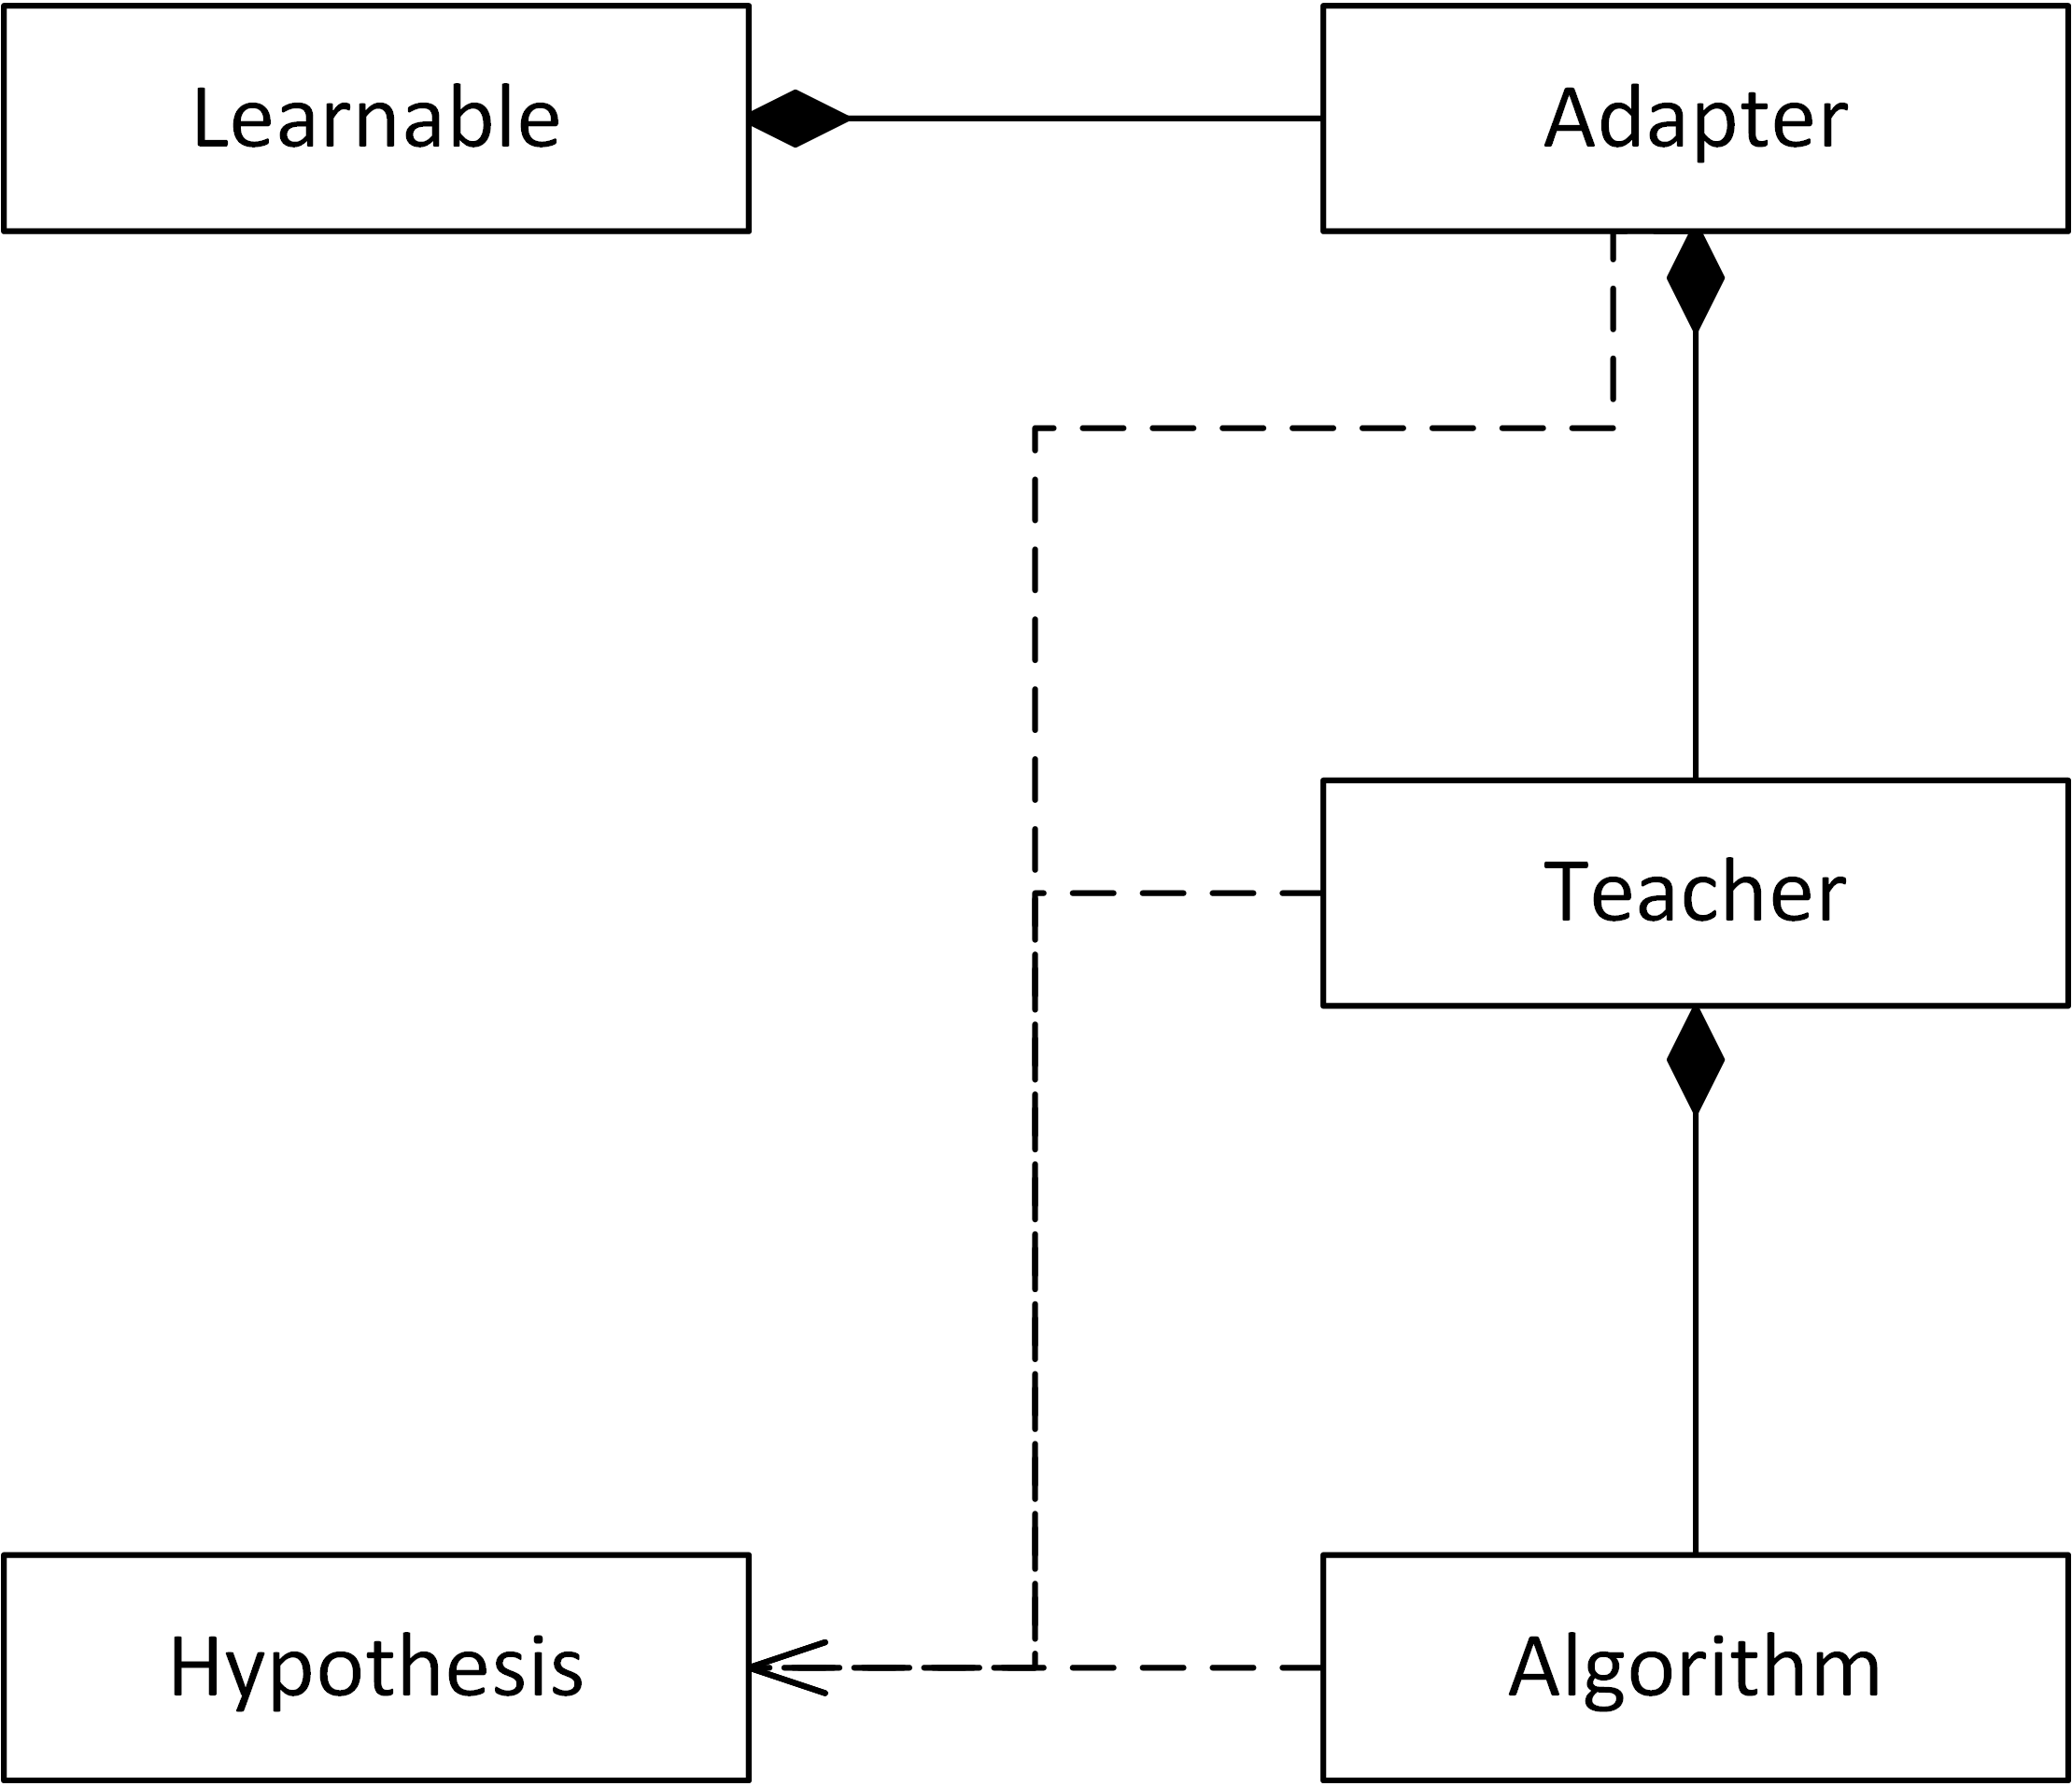
\includegraphics[width=75mm, keepaspectratio]{figures/automatalearning_packages.png}
	%}
	\caption{Structure and relations of the packages comprising the Automata Learning Framework TODO:REF BSC} 
	\label{fig_automatalearning_packages}
\end{figure}

\smallskip

%----------------------------------------------------------------------------
\section{Interactive Learning Framework} \label{sec_interactivelearningframework}
%----------------------------------------------------------------------------
%TODO: random bevezeto szoveg + fig 4.1 kiterjesztett változata - szagatott részekkel keretezve pl az Oracle

%----------------------------------------------------------------------------
\subsection{The Oracle} \label{subsec_oracleimpl}
%----------------------------------------------------------------------------
%TODO: interactive learnable -> LTLparser -> LTLEcoreMetaModel etc.
%TODO: interactiveLearnable Commandok
%TODO: parser - event semantic serializer
%TODO: Ecore ???
%----------------------------------------------------------------------------
\subsection{The Learning Algorithm} \label{subsec_adaptivedhc}
%----------------------------------------------------------------------------
%TODO: DHC, adaptive teacher

%----------------------------------------------------------------------------
\subsection{Caching} \label{subsec_memoization}
%----------------------------------------------------------------------------
%TODO: memoizinglearnable


%----------------------------------------------------------------------------
\chapter{Case Study: Pedestrian Crossing} \label{casestudy}
%----------------------------------------------------------------------------

This section demonstrates the capabilities and limitations of the framework. It presents a problem commonly modeled using state-based models, which is complex enough to demonstrate all aspects of the designed Interactive Learning Entity, but also simple enough to solve - thus verify - only using some background knowledge and common sense. The case study was inspired by the example seen in \cite{molnar2018gamma}.

%---------------------------------------------------------------
\section{Introduction} \label{subs_casestudyintro}
%---------------------------------------------------------------

The problem to solve is modeling a pedestrian crossing with a standard traffic light and a pedestrian light as illustrated on Figre \ref{fig_casestudy_systemstates}. As the traffic lights and the pedestrian lights on the opposite sides of the crossing behave identically, we are going to model only one instance of each device. 

The traffic light is looping through the red-green-yellow-red sequence. As an extra, there is an interrupted mode that may be triggered by the police, which results in blinking yellow light. The pedestrian light loops through the red-green-red sequence, and turns black when an interrupt arrives. A subsequent interrupt turns the lights back on, also considering that the sytem must always be in a safe state - i.e. the lights must not allow passage for both the pedestrians and the road vehicles at the same time.

\begin{figure}[!ht] 
	\centering
	\fbox{
		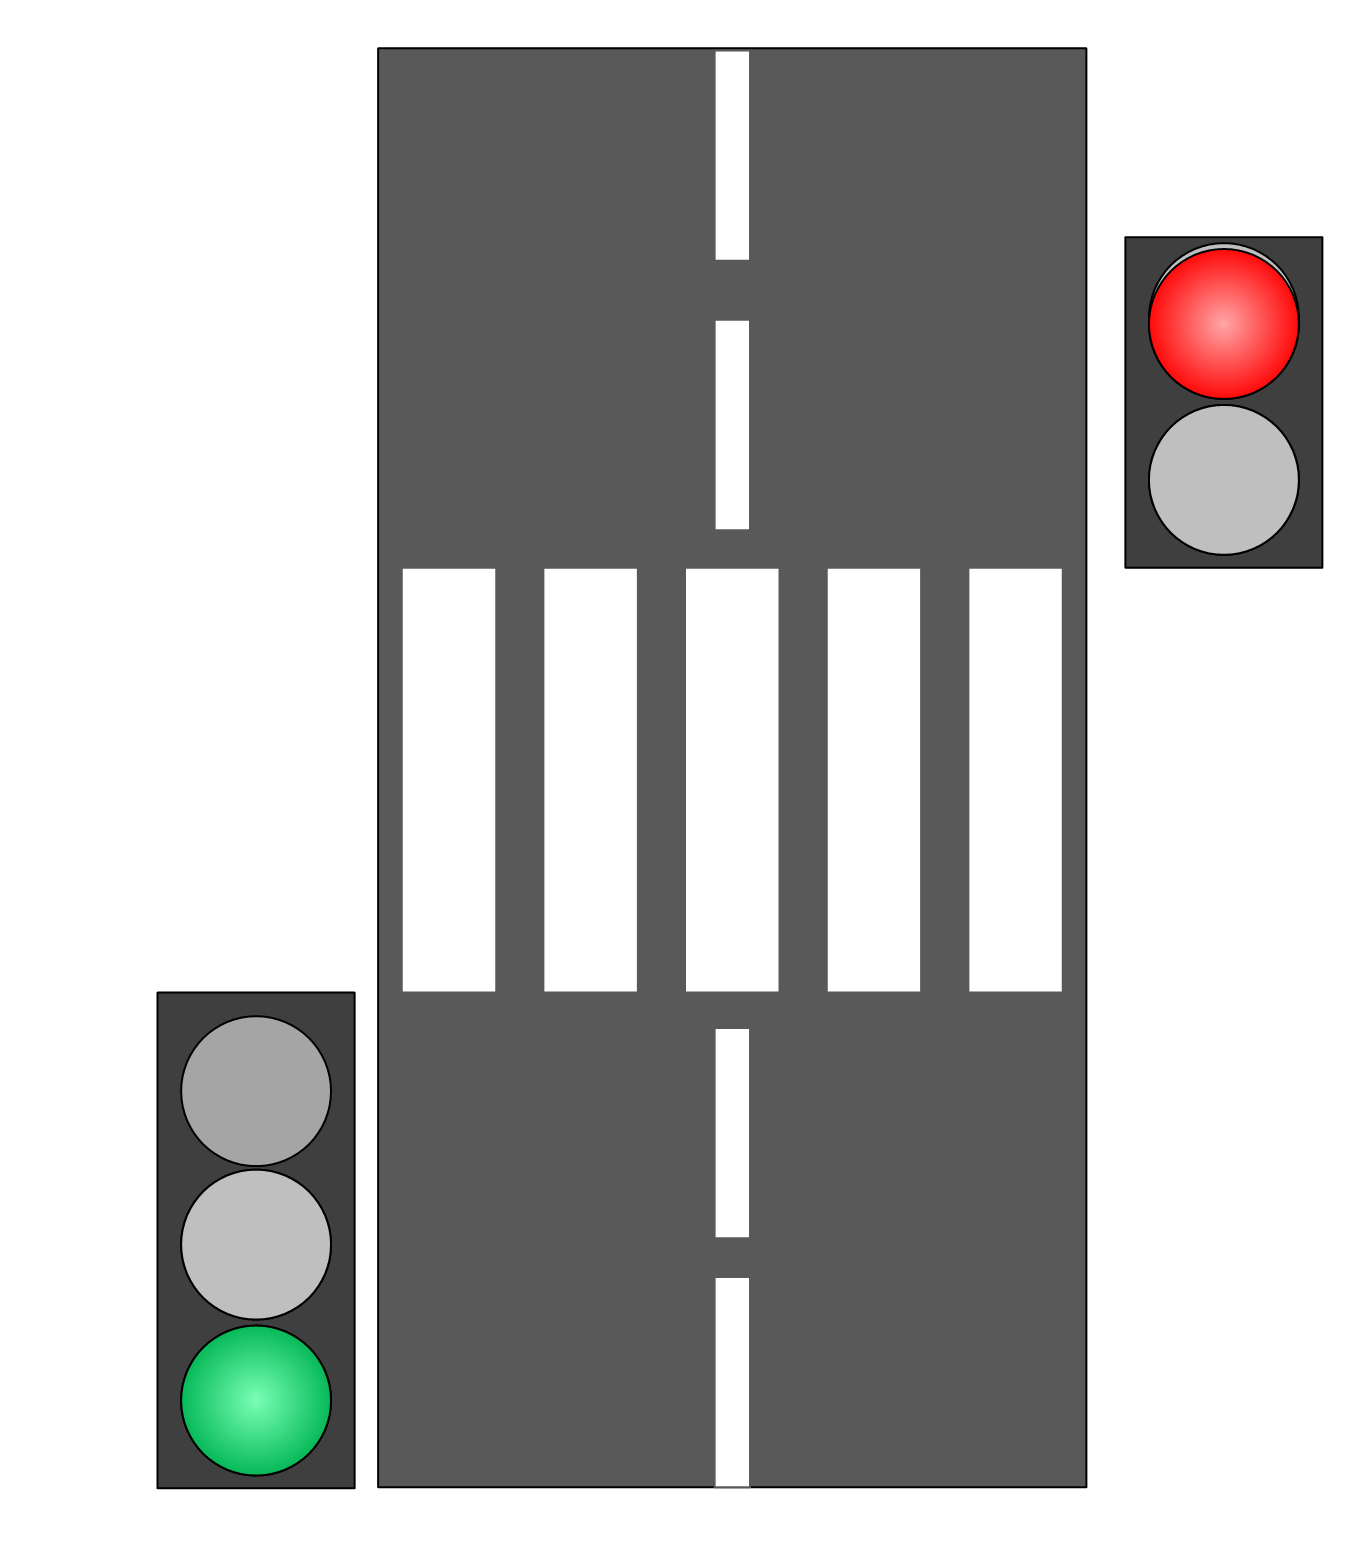
\includegraphics[width=30mm, keepaspectratio]{figures/casestudy_state1.png}
	}
	\fbox{
		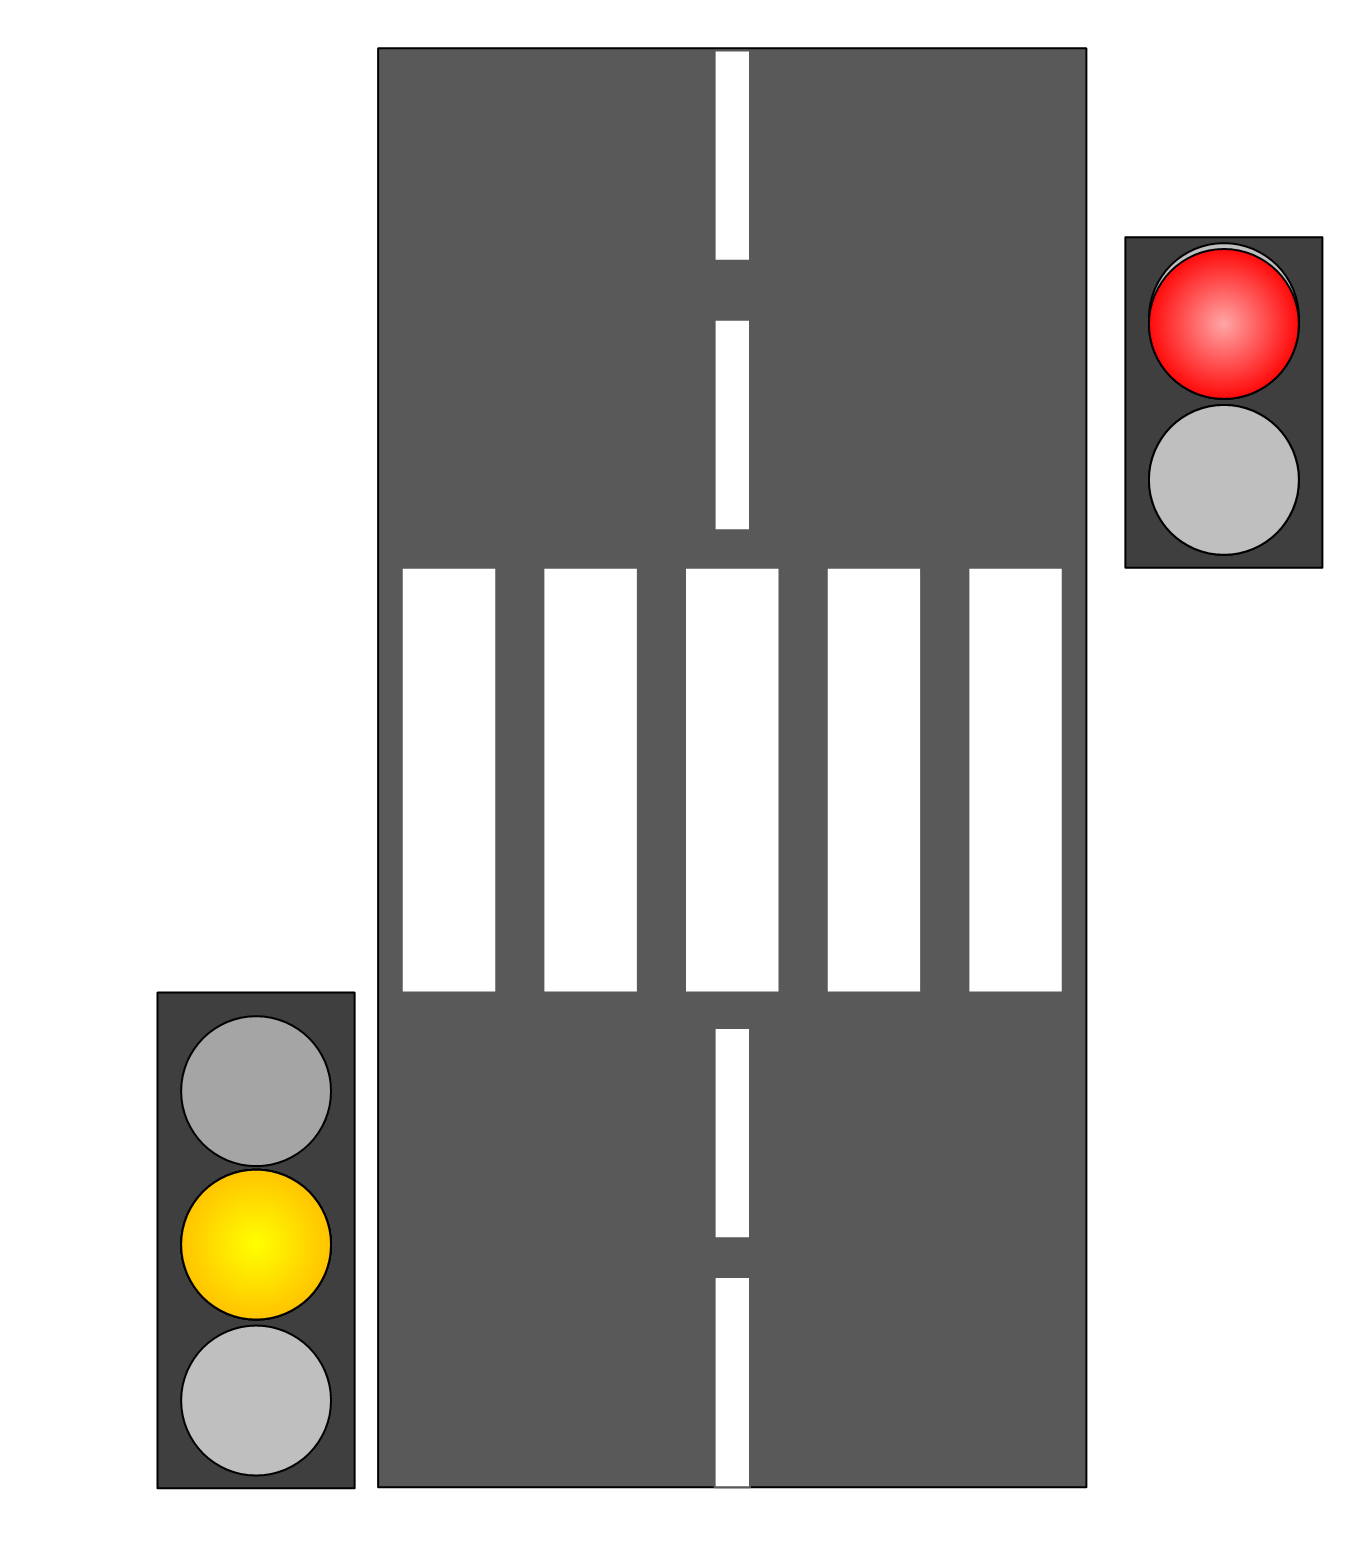
\includegraphics[width=30mm, keepaspectratio]{figures/casestudy_state2.png}
	}
	\fbox{
		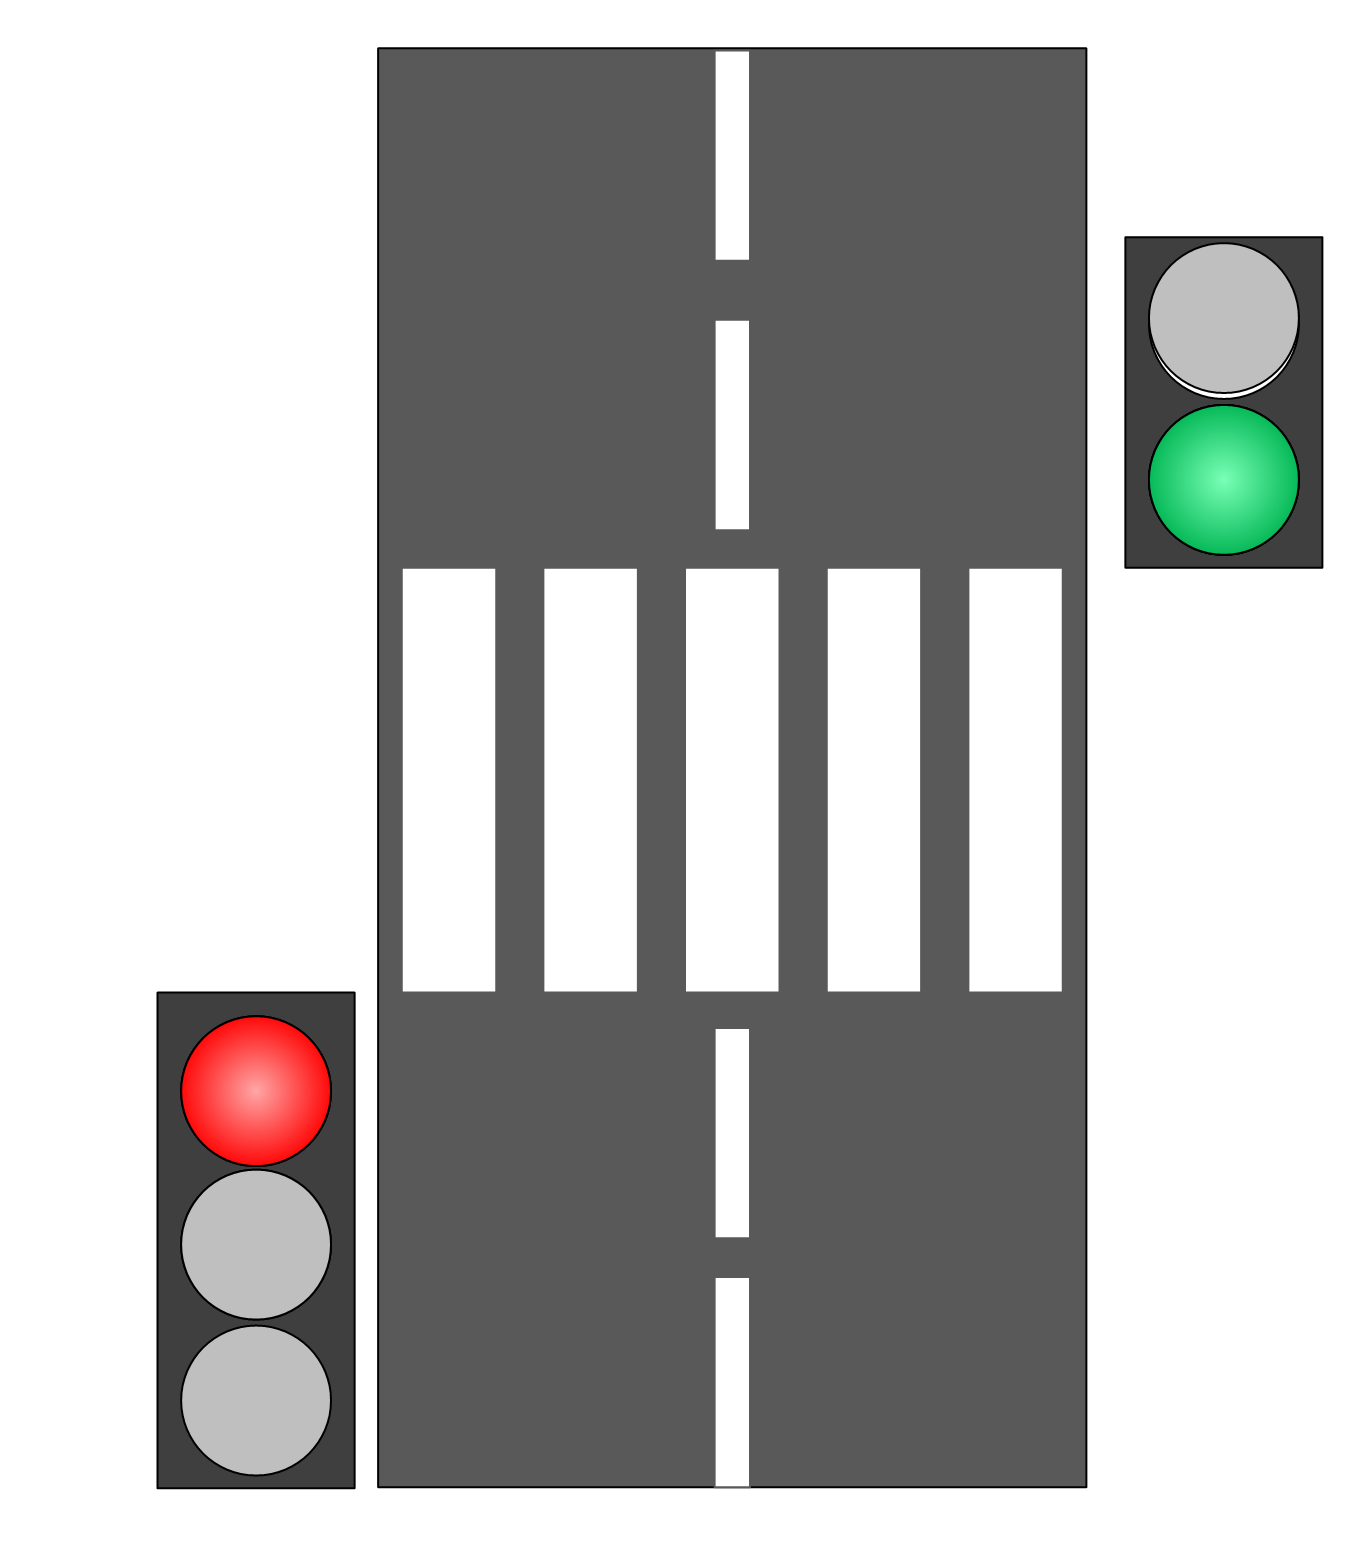
\includegraphics[width=30mm, keepaspectratio]{figures/casestudy_state3.png}
	}
	\fbox{
		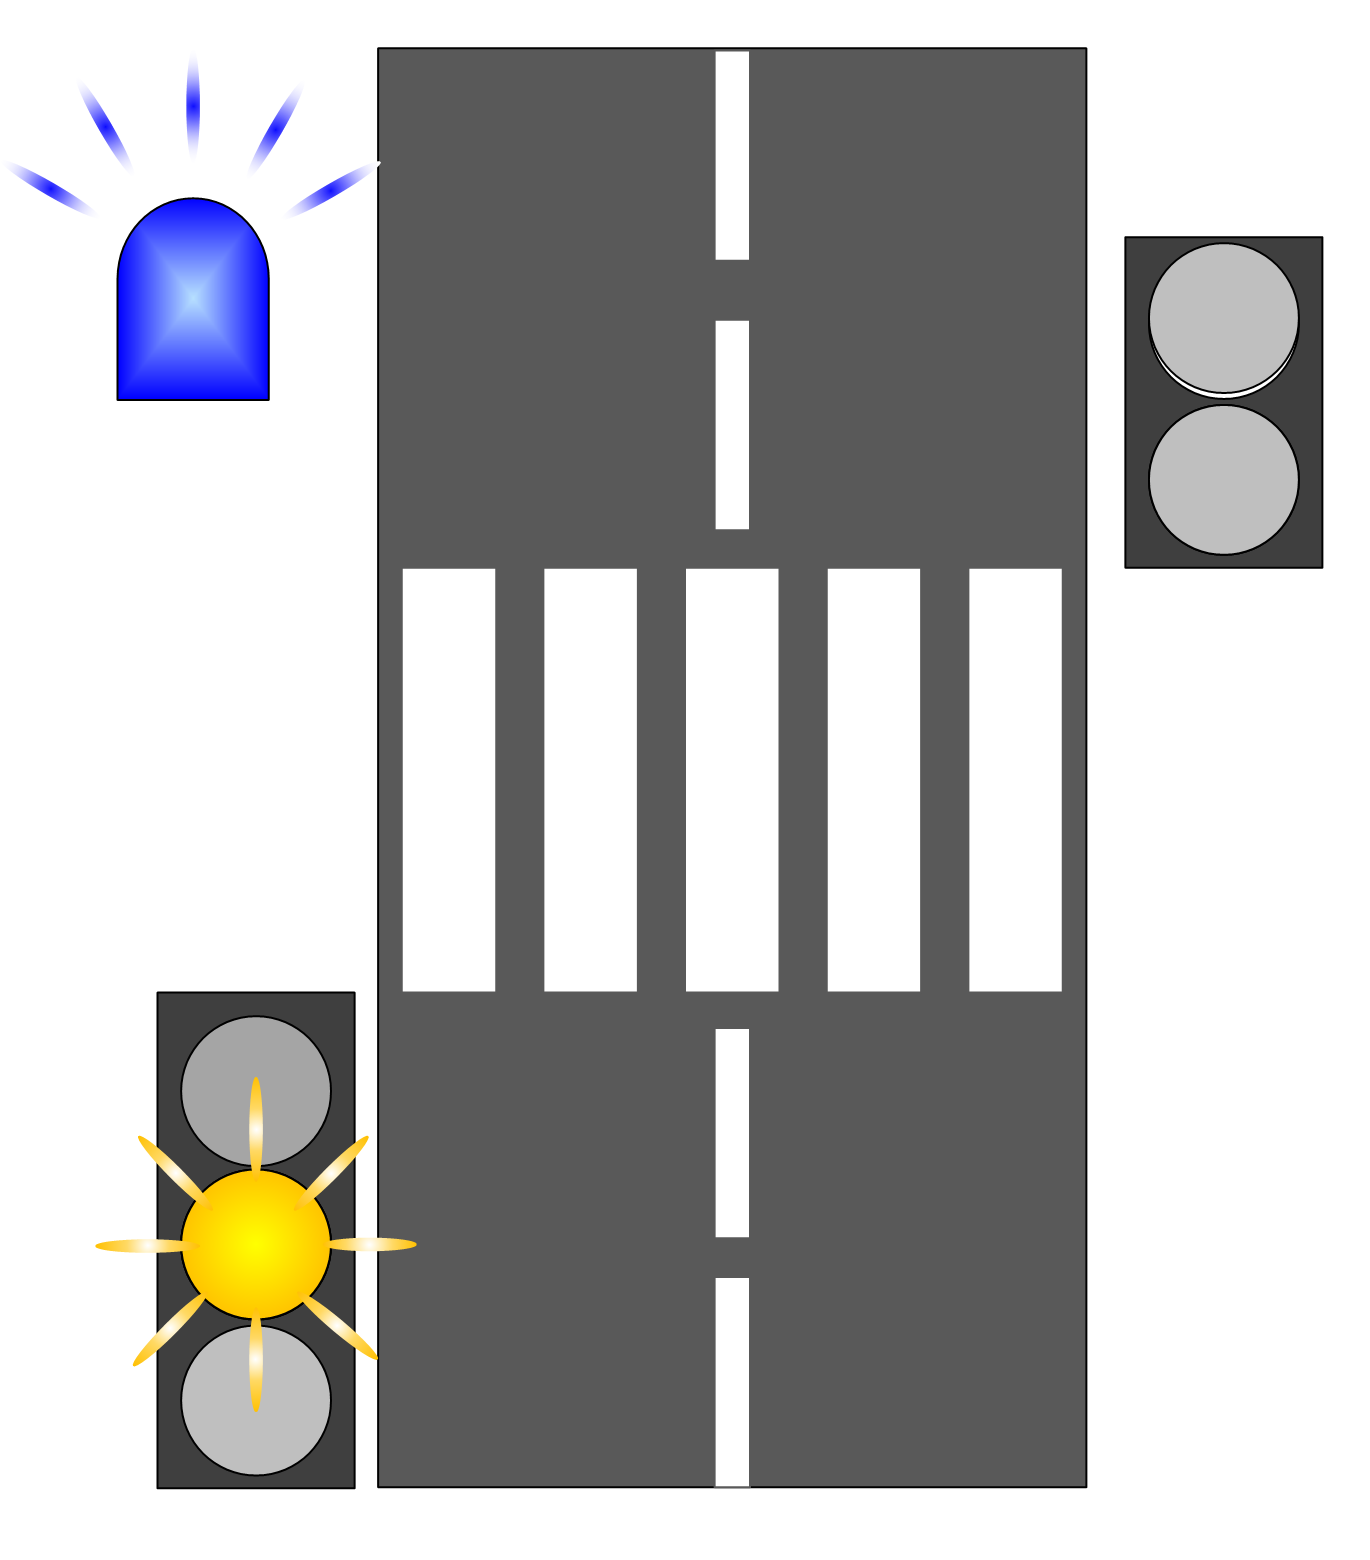
\includegraphics[width=30mm, keepaspectratio]{figures/casestudy_state4.png}
	}
	\caption{Possible states of the system: normal operation (\textit{three from the left}) and the interrupted state \textit{(right)}} 
	\label{fig_casestudy_systemstates}
\end{figure}

%---------------------------------------------------------------
\section{Component Design} \label{subs_casestudycomps}
%---------------------------------------------------------------

The previous subsection mentioned two components of the composite system: a traffic light and a pedestrian light. To realize the safe state of the system, the components must synchronize their behavior, justificating the existence of a third, controller component. The traffic and pedestrian light components should have one input and one output port -- they  are relatively simple -- and the controller should have an input port for the police and two output ports for the components.

\textbf{The traffic light component} has two possible inputs on its input port (TrafficControl) - toggle and interrupt - and four outputs on its output port (TrafficDisplay) - red, green, yellow and blinking yellow - as it appeared in the problem description.

\textbf{The pedestrian light component} has the same two inputs on its input port (PedestrianControl) - toggle and interrupt - and three outputs on its output port (PedestrianDisplay) - red, green, and black - as it appeared in the problem description.

\textbf{The controller component} controls the rhythm of the change of states and also interrupts the other components when the police interrupt arrives. It has an input port ('\textit{Police}') for the police interrupt and two output ports ('\textit{TrafficControl}' and '\textit{PedestrianControl}') - matching the input ports of the other components.

The described components and their connections are illustrated on Figure \ref{fig_casestudy_blockdiagram}.

\begin{figure}[!ht] 
	\centering
	%\fbox{
	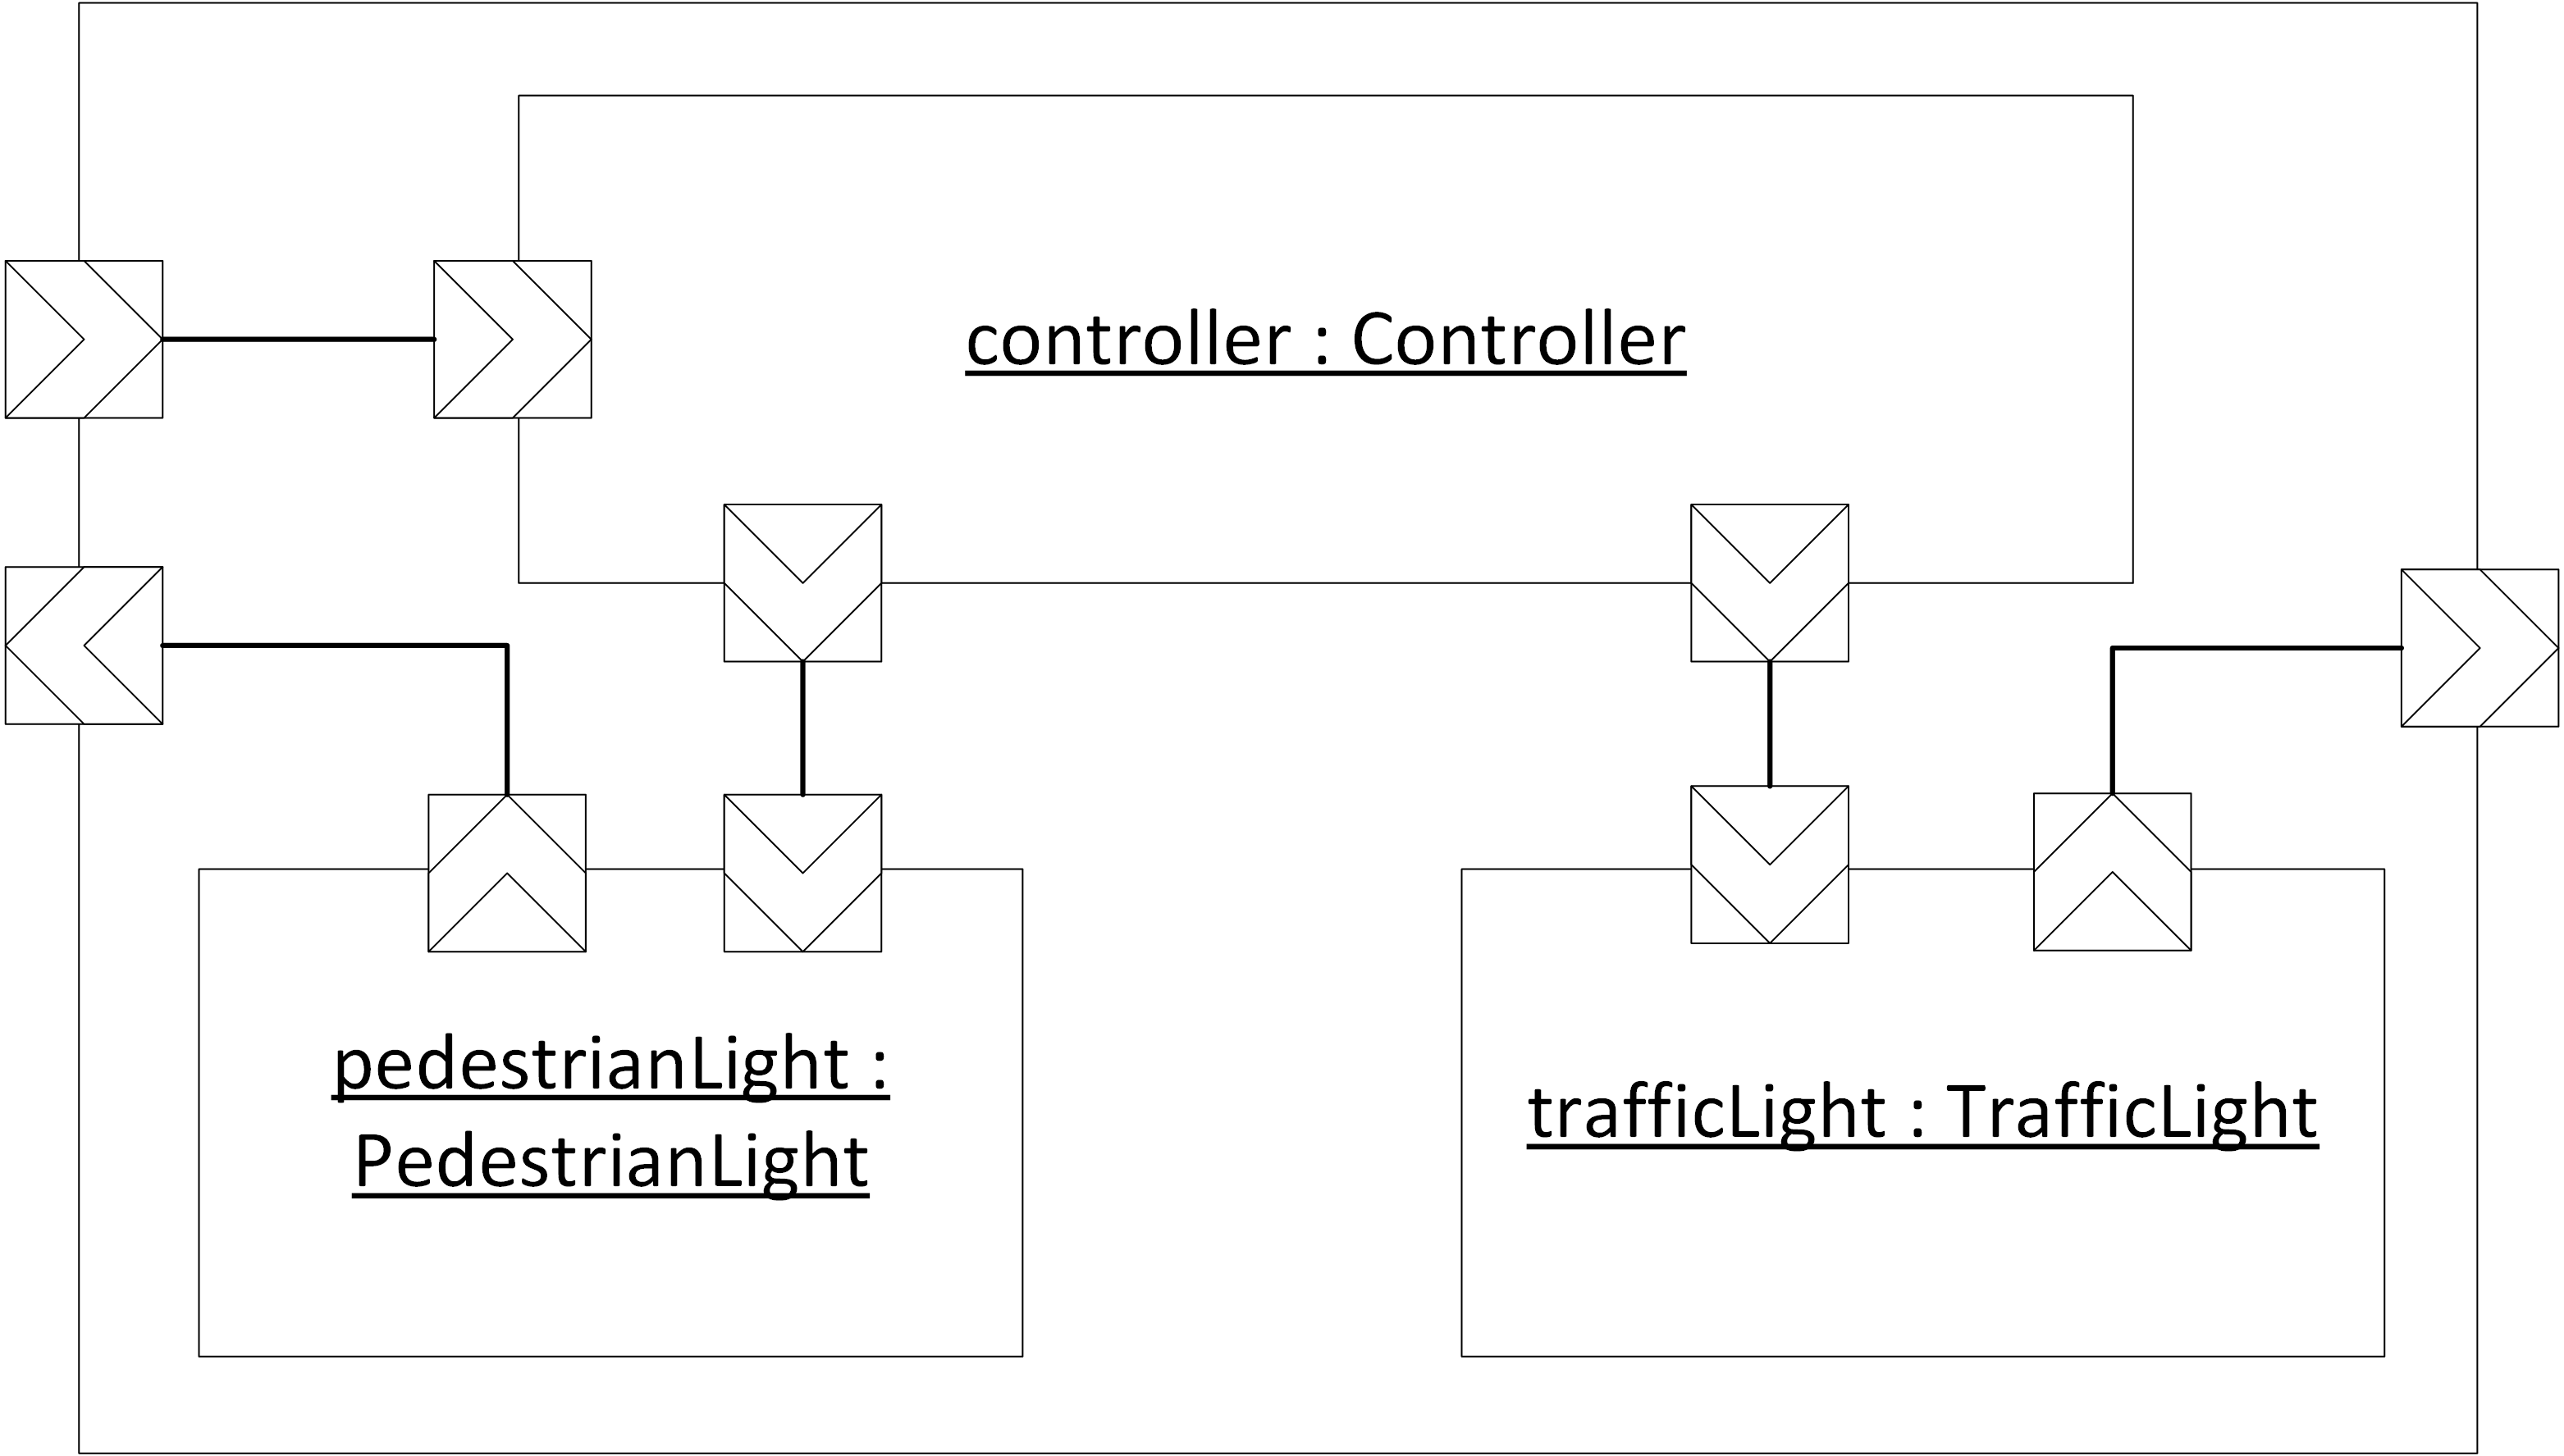
\includegraphics[width=130mm, keepaspectratio]{figures/casestudy_blockdiagram.png}
	%}
	\caption{Components of the modeled system and their connections} 
	\label{fig_casestudy_blockdiagram}
\end{figure}

\textbf{The Expected Behavior of the Components} 

The components have been separated and their interfaces precisely defined, thus, we can proceed to formulating behavior-related requirements. For instance, the traffic light component must conform to the following -- not exhaustive -- list:

\begin{itemize}
	\item The traffic light must loop through the sequence 'toggle/red toggle/green toggle/yellow toggle/red' during normal operation.
	\item The traffic light must display blinking yellow signal when a police interrupt arrives during normal operation.
	\item The traffic light must return to normal operation when a second interrupt arrives.
	\item The traffic light must display red signal when returning to normal operation.
	\item The traffic light must always display blinking yellow when interrupted. 
	
\end{itemize}

A very similar list can be constructed for the pedestrian light component. The controller component is slightly more complicated, as it may toggle or interrupt the other components at the same time, so its alphabet shall contain separate elements for these cases.

%---------------------------------------------------------------
\section{Synthesizing the Components} \label{subs_casestudysynth}
%---------------------------------------------------------------

Now we add the previously formulated requirements to the ILE, in formalisms that it is able to interpret. In the following examples for the interaction of the user with the ILE, '$\circ$' symbolizes the ILE and '$\triangleright$' symbolizes the user (interface qualifications are omitted for shorter and simpler expressions). 

\bigskip
\fbox{
	\parbox{\textwidth}{
		\begin{itemize}
			\setlength\itemsep{0.2em}
			\item[$\circ$] Provide the requirements for component 'TrafficLight':
			\item[$\triangleright$] Valid Trace: toggle/red toggle/green toggle/yellow toggle/red
			\item[$\triangleright$] LTL Expression: F(interrupt -> X(G(toggle) -> G(blinkingYellow)))
			\item[$\triangleright$] Invalid Trace: interrupt/red interrupt/blinkingYellow
			\item[$\triangleright$] LTL Expression: F(G(interrupt -> (blinkingYellow | red)))
			
			\smallskip
			... other components ...
		\end{itemize}
	}
}

\bigskip
After adding these requirements during the offline phase, the synthesis of the components can proceed to the online, interactive phase. A possible run of the learning process can be seen below.

\bigskip
\fbox{
	\parbox{\textwidth}{
		\begin{itemize}
			\setlength\itemsep{0.2em}
			\item[$\circ$] Learning component 'TrafficLight'
			\item[$\circ$] Provide the output for sequence [toggle, interrupt]:
			\item[$\triangleright$] Corresponding Output: blinkingYellow
			\item[$\circ$] Provide the output for sequence [toggle, interrupt, interrupt]:
			\item[$\triangleright$] Corresponding Output: red
			\item[$\circ$] Provide the output for sequence [toggle, toggle, interrupt]:
			\item[$\triangleright$] Corresponding Output: blinkingYellow
			\item[$\circ$] Provide the output for sequence [toggle, toggle, interrupt, interrupt]:
			\item[$\triangleright$] Corresponding Output: red
			\item[$\circ$] Provide the output for sequence [toggle, toggle, toggle, interrupt]:
			\item[$\triangleright$] Corresponding Output: blinkingYellow
			\item[$\circ$] Equivalence Query (Figure \ref{fig_trafficlightincomplete} in the Appendix)
			\item[$\triangleright$] Counterexample: interrupt interrupt
			\item[$\circ$] Provide the output for sequence [interrupt, interrupt, interrupt]:
			\item[$\triangleright$] Valid Trace: interrupt/blinkingYellow interrupt/red interrupt/blinkingYellow interrupt/red
			\item[$\circ$] Provide the output for sequence [interrupt, interrupt, toggle]:
			\item[$\triangleright$] Corresponding Output: green
			\item[$\circ$] Provide the output for sequence [interrupt, toggle, interrupt]:
			\item[$\triangleright$] Corresponding Output: red
			\item[$\circ$] Equivalence Query (Figure \ref{fig_casestudy_trafficlightlearned})
			\item[$\triangleright$] Approved.
			
			\smallskip
			... other components ...
		\end{itemize}
	}
}

\bigskip
The same learning process can be seen on Listing \ref{lst_examplelearning} in the Appendix, which presents the inputs and outputs as they appeara on the command line interface.

%---------------------------------------------------------------
\section{The Learned Models} \label{subs_casestudyresults}
%---------------------------------------------------------------

Now we can examine any differences between the expected and the learned models. Figure \ref{fig_casestudy_trafficlightdiff} presents the expected and the synthesized traffic light models.

\begin{figure}[H] 
	\centering
	\begin{subfigure}[b]{0.9\textwidth}
		\centering
		\fbox{
			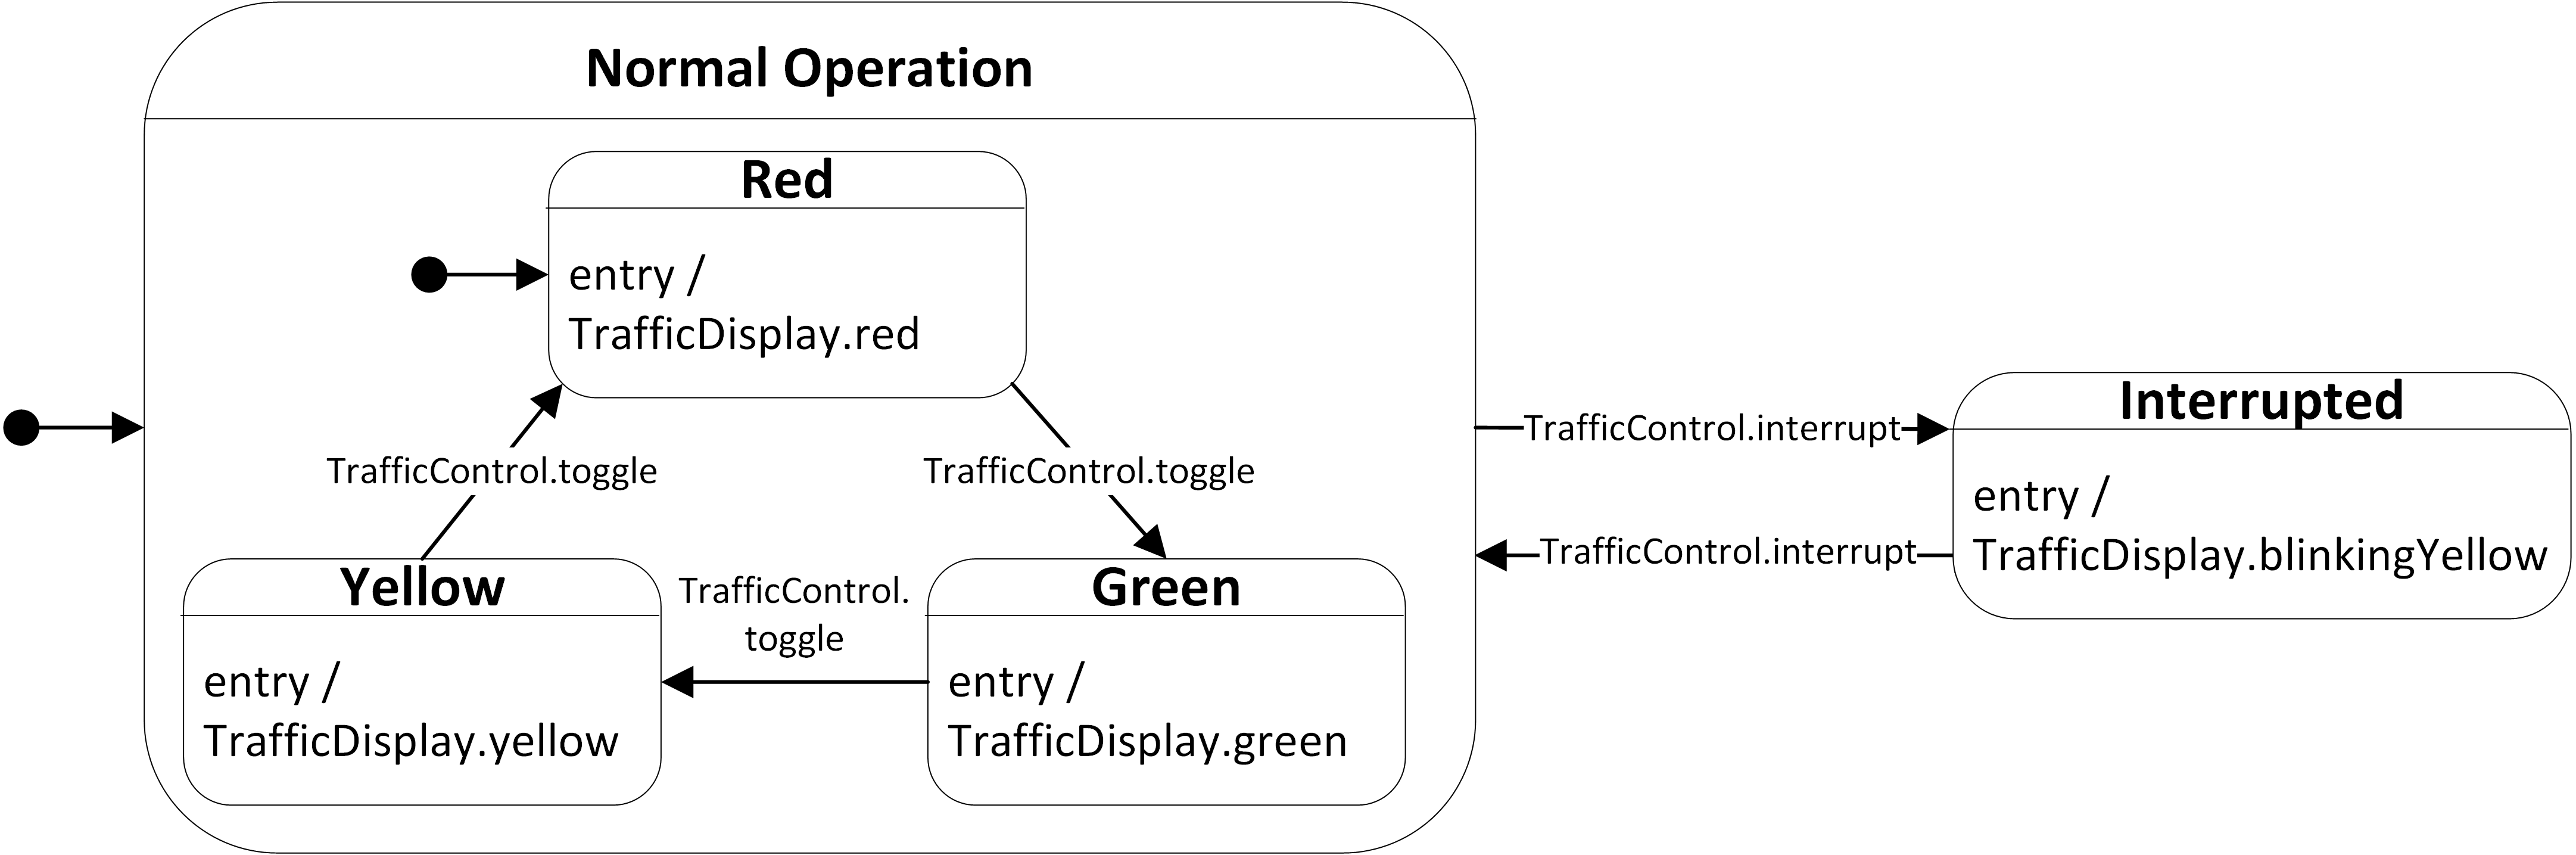
\includegraphics[width=120mm]{figures/casestudy_trafficlightexpected.png}
		}	
		\caption{Expected}
	\end{subfigure}
	\hfill
	\begin{subfigure}[b]{0.9\textwidth}
		\centering
		\fbox{
			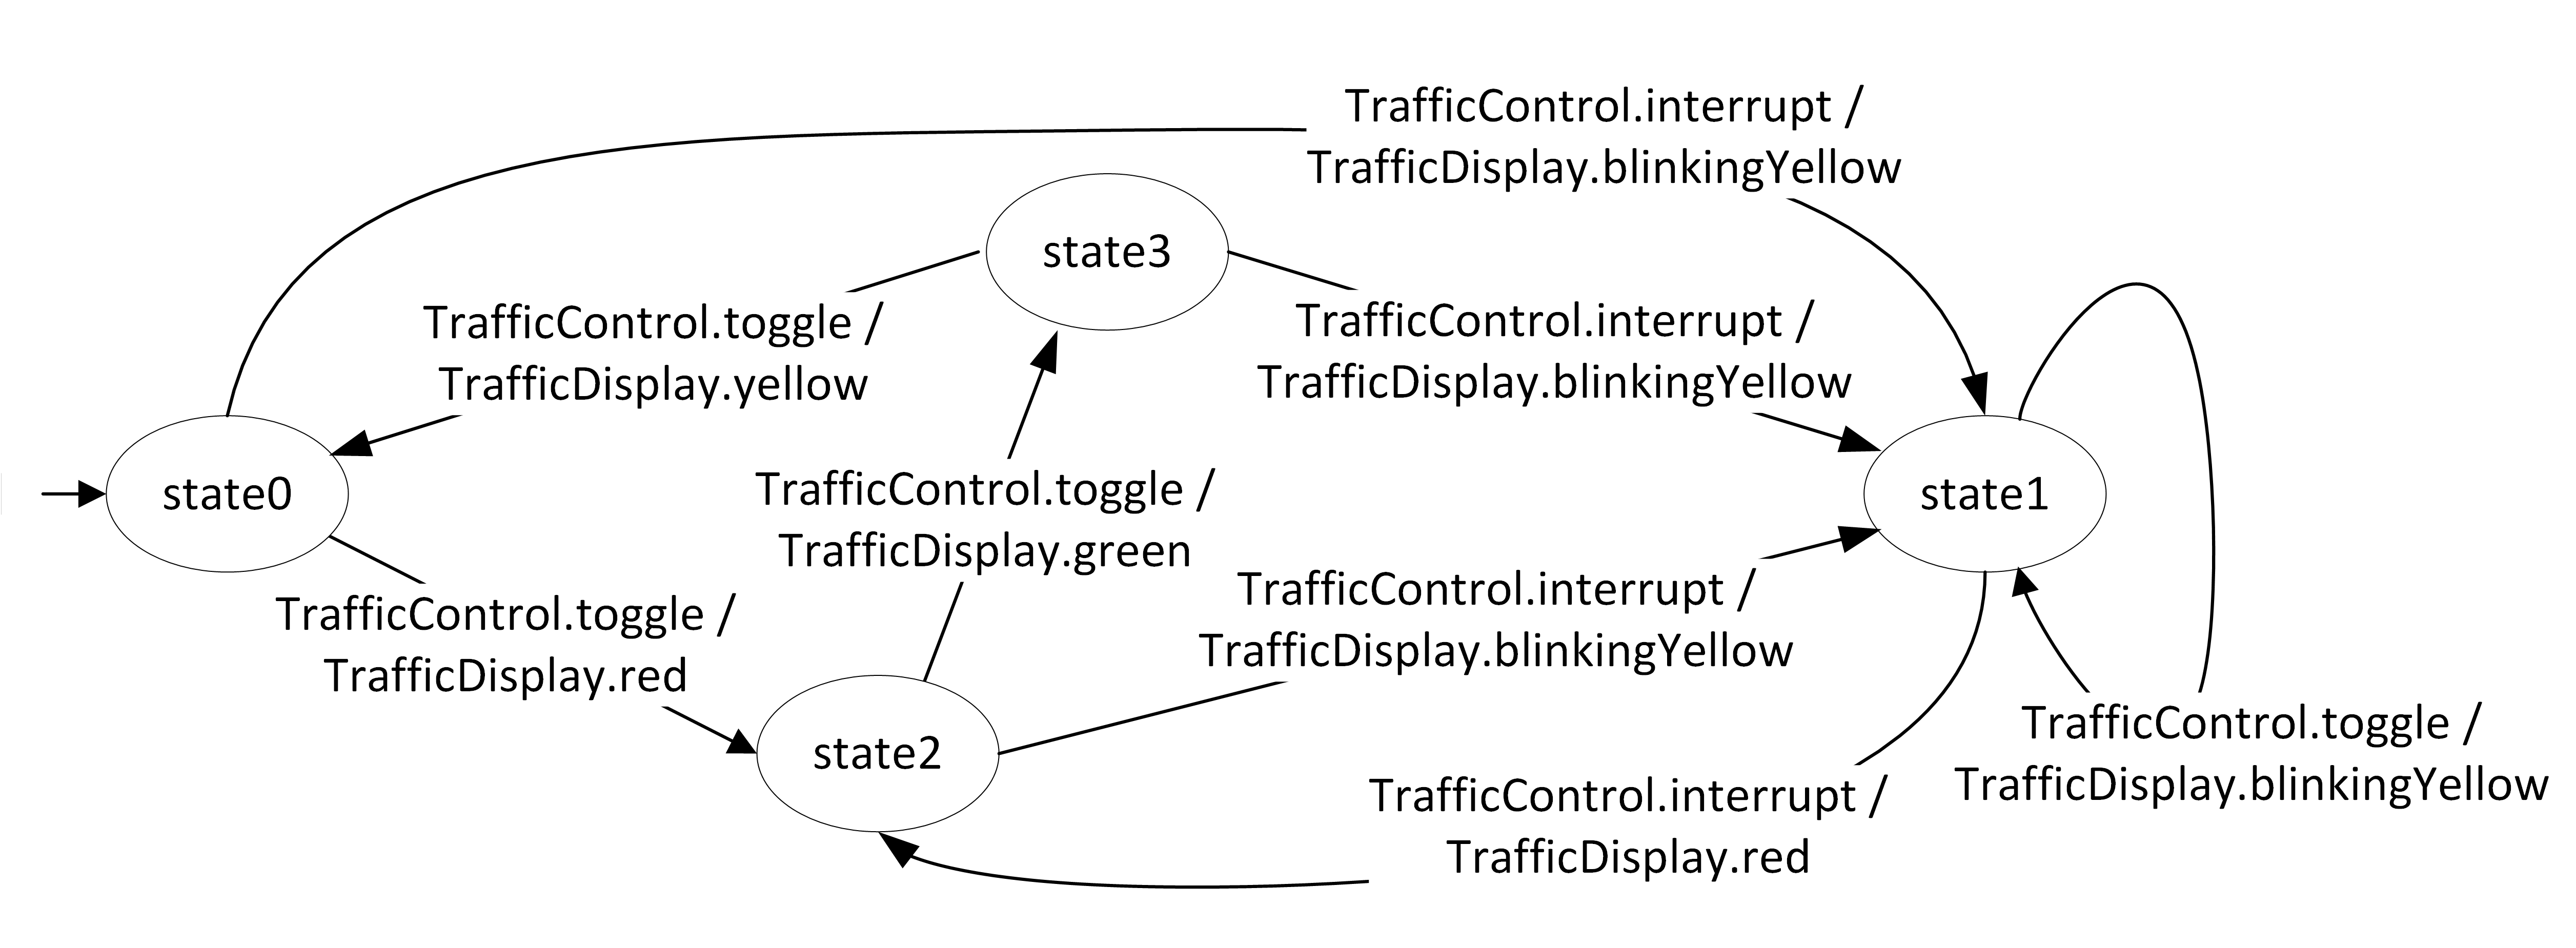
\includegraphics[width=120mm]{figures/casestudy_trafficlightlearned.png}
		}
		\caption{Learned}	
		\label{fig_casestudy_trafficlightlearned}
	\end{subfigure}
	\caption{The expected and the learned traffic light models}
	\label{fig_casestudy_trafficlightdiff}
\end{figure}

The structure of the models is clearly different, notably:
\begin{itemize}
	\item The expected models contain hierarchical states, while the learned ones are 'flat'.
	\item The expected models also contain entry and exit actions, while the learned models only contain actions on transitions. 
	\item The expected models contain meaningful state names, while the learned ones only have generated ones.
\end{itemize}

However, the models are behaviorally equivalent. Both models meet the requirements stated in Subsection \ref{subs_casestudycomps}, and after careful examination, it is obvious that the only initial states are different -- as no entry actions are used in the learned models -- and the transition starting from the hierarchical state is separated into three different transitions.

The differences between the expected and learned pedestrian light components can be seen on Figure \ref{fig_casestudy_pedestrianlightdiff}. The differences are the similar to those of the traffic light models, as the modeled behavior is also very similar. 

\begin{figure}[!ht] 
	\centering
	\begin{subfigure}[b]{0.9\textwidth}
		\centering
		\fbox{
			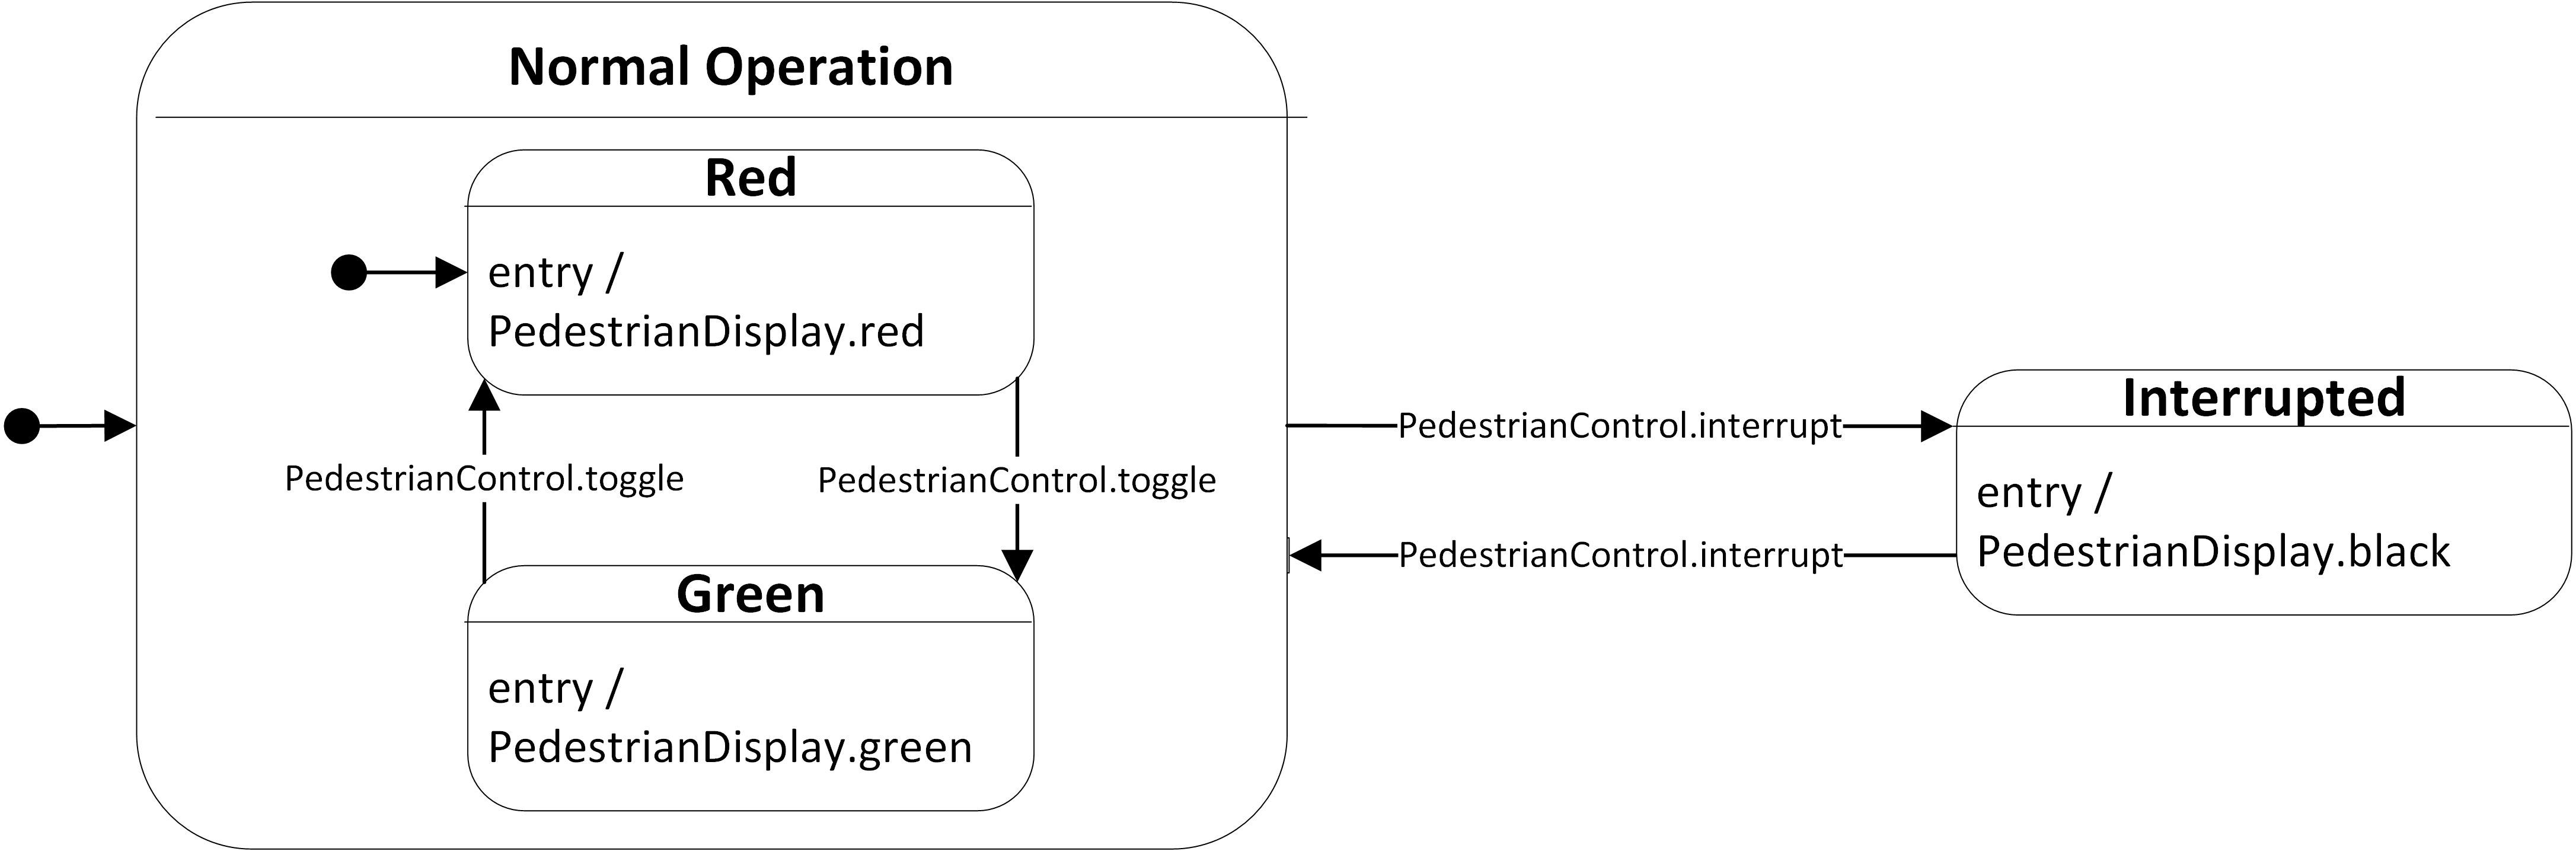
\includegraphics[width=120mm]{figures/casestudy_pedestrianlightexpected.png}
		}	
		\caption{Expected}
	\end{subfigure}
	\hfill
	\begin{subfigure}[b]{0.9\textwidth}
		\centering
		\fbox{
			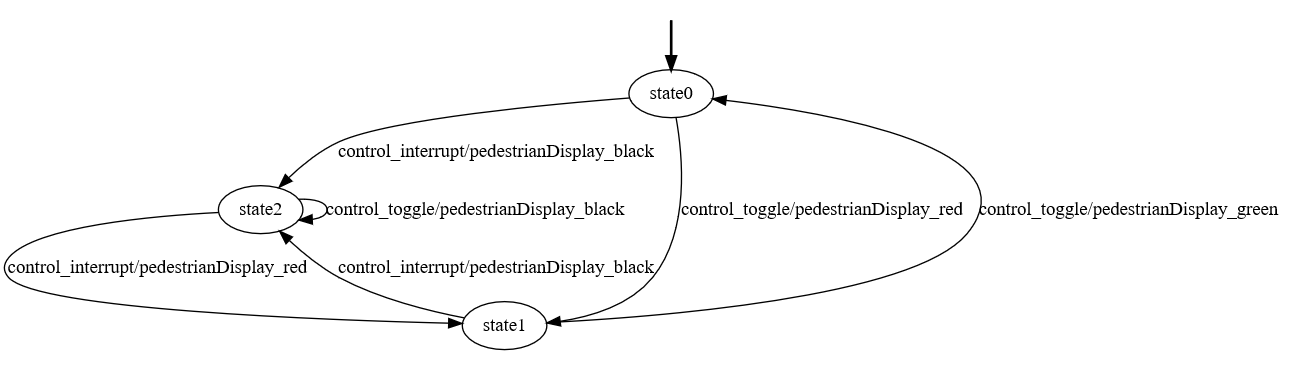
\includegraphics[width=120mm]{figures/casestudy_pedestrianlightlearned.PNG}
		}
		\caption{Learned}	
	\end{subfigure}
	\caption{The expected and the learned pedestrian light models}
	\label{fig_casestudy_pedestrianlightdiff}
\end{figure}

The behavior of the controller component can be learned similarly. The expected and the synthesized models can be seen on Figure \ref{fig_casestudy_controllerdiff}. Note, that in addition to '{\fontfamily{qcr}\selectfont Police.interrupt}', the component also has an unqualified t input word. This represents a timeout event the engineer must extend the serialized model with -- but acts as a regular input event during the learning. 

\begin{figure}[!ht] 
	\centering
	\begin{subfigure}[b]{0.9\textwidth}
		\centering
		\fbox{
			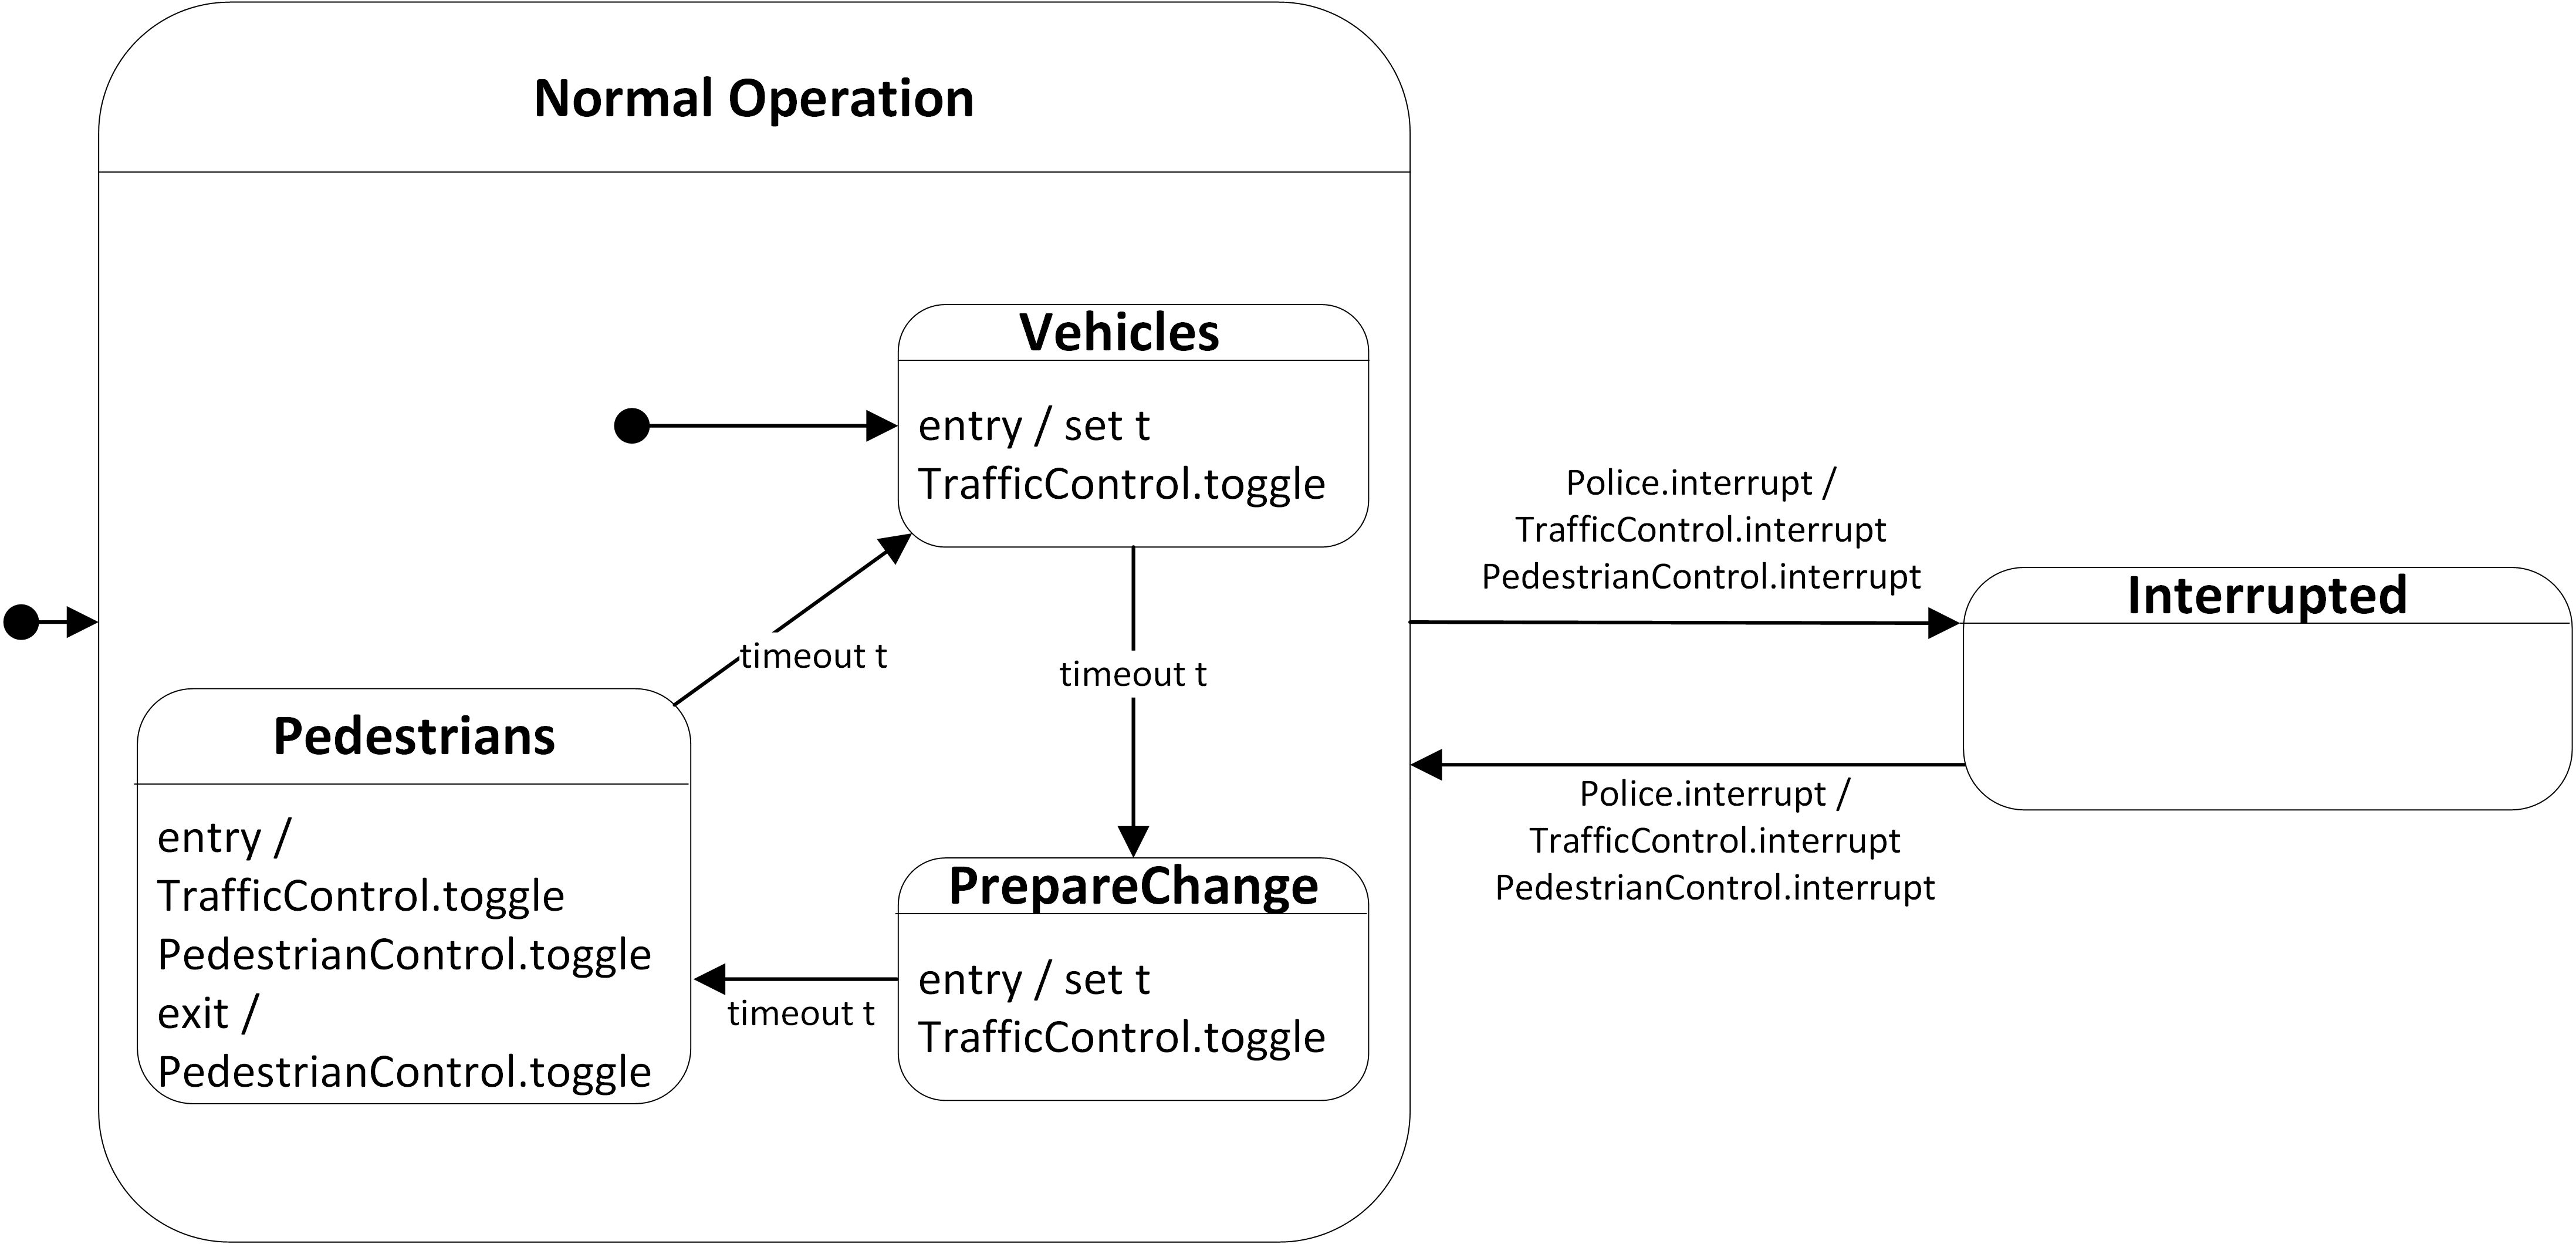
\includegraphics[width=120mm]{figures/casestudy_controllerexpected.png}
		}	
		\caption{Expected}
	\end{subfigure}
	\hfill
	\begin{subfigure}[b]{0.9\textwidth}
		\centering
		\fbox{
			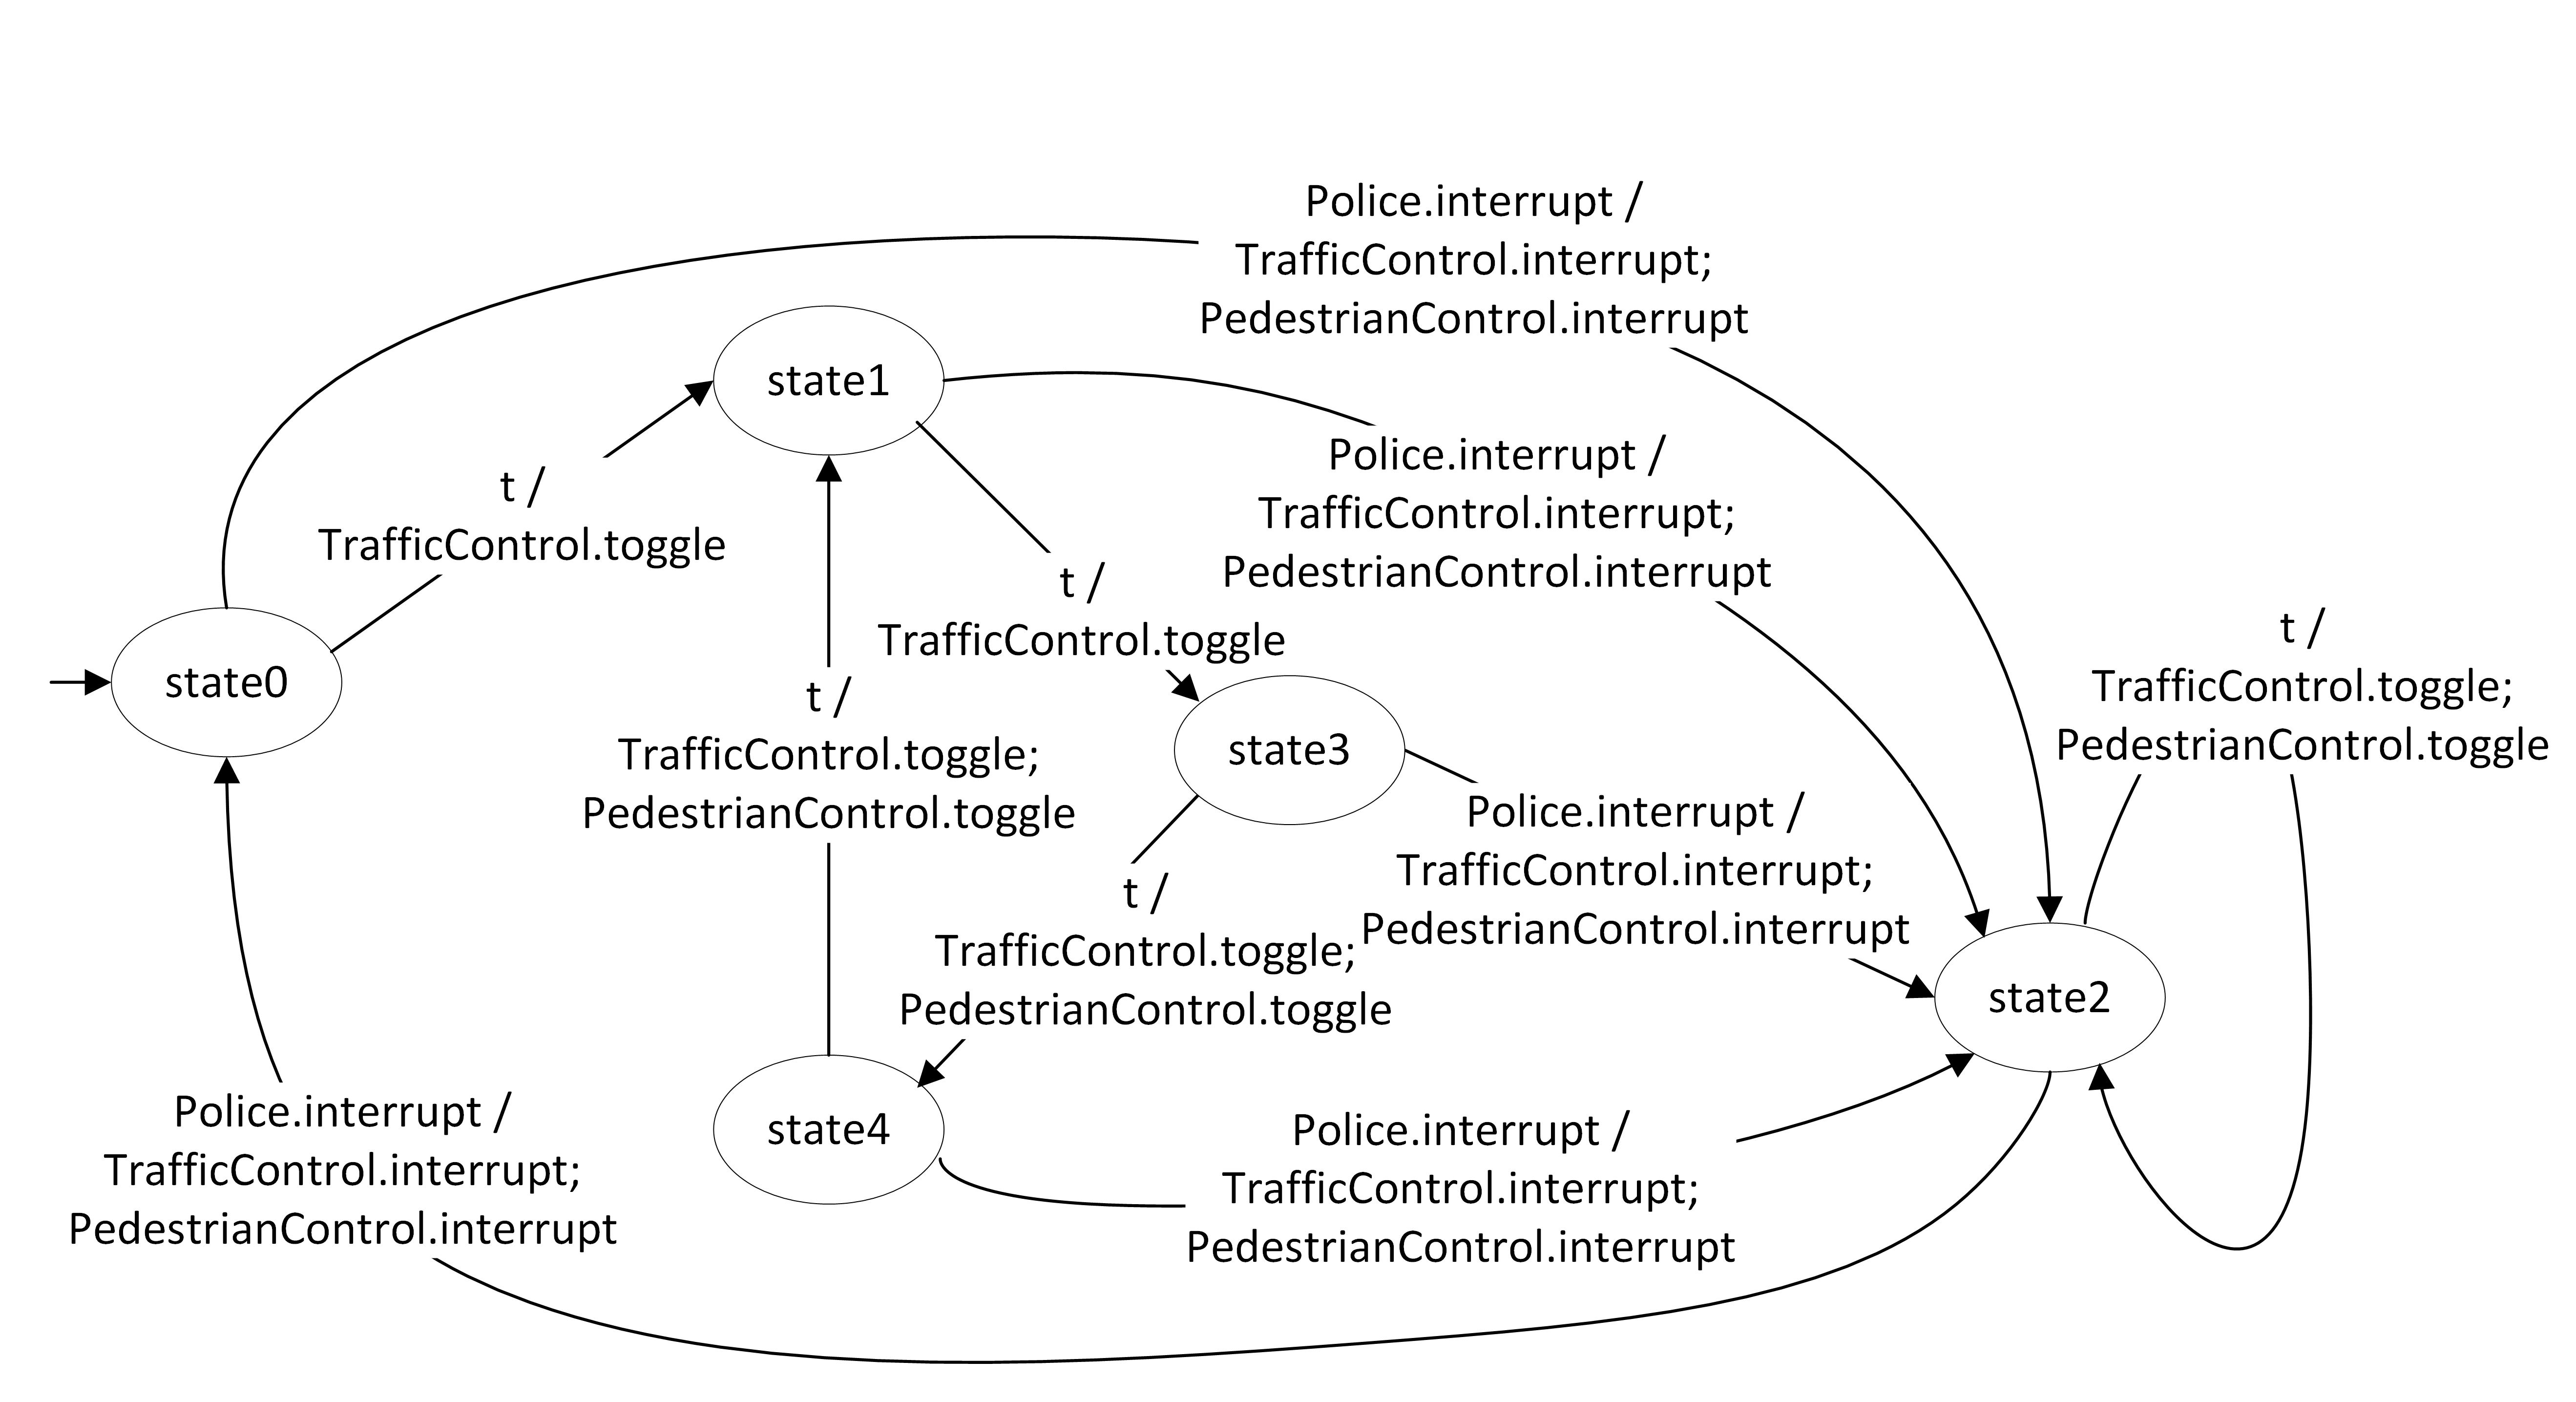
\includegraphics[width=120mm]{figures/casestudy_controllerlearned.png}
		}
		\caption{Learned}	
	\end{subfigure}
	\caption{The expected and the learned controller models}
	\label{fig_casestudy_controllerdiff}
\end{figure}

After learning every component, the collection of the models is serialized as a Gamma project, with the following files and contents:
\begin{itemize}
	\item TrafficLight.gcd (the learned traffic light component)
	\item PedestrianLight.gcd (the learned pedestrian light component)
	\item Controller.gcd (the learned controller component)
	\item CompositeSystem.gcd (connections between the component ports, as illustrated on Figure \ref{fig_casestudy_blockdiagram})
	\item Interfaces.gcd (the interface definitions based on the ports of the components)
\end{itemize}
After extending the controller with statechart-specific elements (namely the timeout event), the engineer can use the Gamma Framework\cite{DBLP:conf/icse/MolnarGVMV18} to check the correctness of the system model or even generate implementation code.



%----------------------------------------------------------------------------
\chapter{Evaluation}
%----------------------------------------------------------------------------
This chapter presents the applicability of the designed framework, evaluates its current capabilities and points out improvement possibilities. Section \ref{sec_theoeval} evaluates the current state of the framework, then Section \ref{sec_casestudy} presents a case study about the applicability of our solution. Lastly, Section \ref{sec_futurework} presents the opportunities for the continuation of the work.

%----------------------------------------------------------------------------
\section{Case Study: Pedestrian Crossing} \label{sec_casestudy}
%----------------------------------------------------------------------------
This section demonstrates the capabilities and limitations of the framework. It presents a problem commonly modeled using state-based models, which is complex enough to demonstrate all aspects of the designed Interactive Learning Entity, but also simple enough to solve - thus verify - only using some background knowledge and common sense. [TODO ref gamma tutorial?]

%---------------------------------------------------------------
\subsection{Introduction} \label{subs_casestudyintro}
%---------------------------------------------------------------

The problem to solve is modeling a pedestrian crossing with a standard traffic light and a pedestrian light as illustrated on Figre \ref{fig_casestudy_systemstates}. As the traffic lights and the pedestrian lights on the opposite sides of the crossing behave identically, we are going to model only one instance of each device. 

The traffic light is looping through the red-green-yellow-red sequence. As an extra, there is an interrupted mode that may be triggered by the police, which results in blinking yellow light. The pedestrian light loops through the red-green-red sequence, and turns black when an interrupt arrives. A subsequent interrupt turns the lights back on, also considering that the sytem must always be in a safe state - i.e. the lights must not allow passage for both the pedestrians and the road vehicles at the same time.

\begin{figure}[!ht] 
	\centering
	\fbox{
		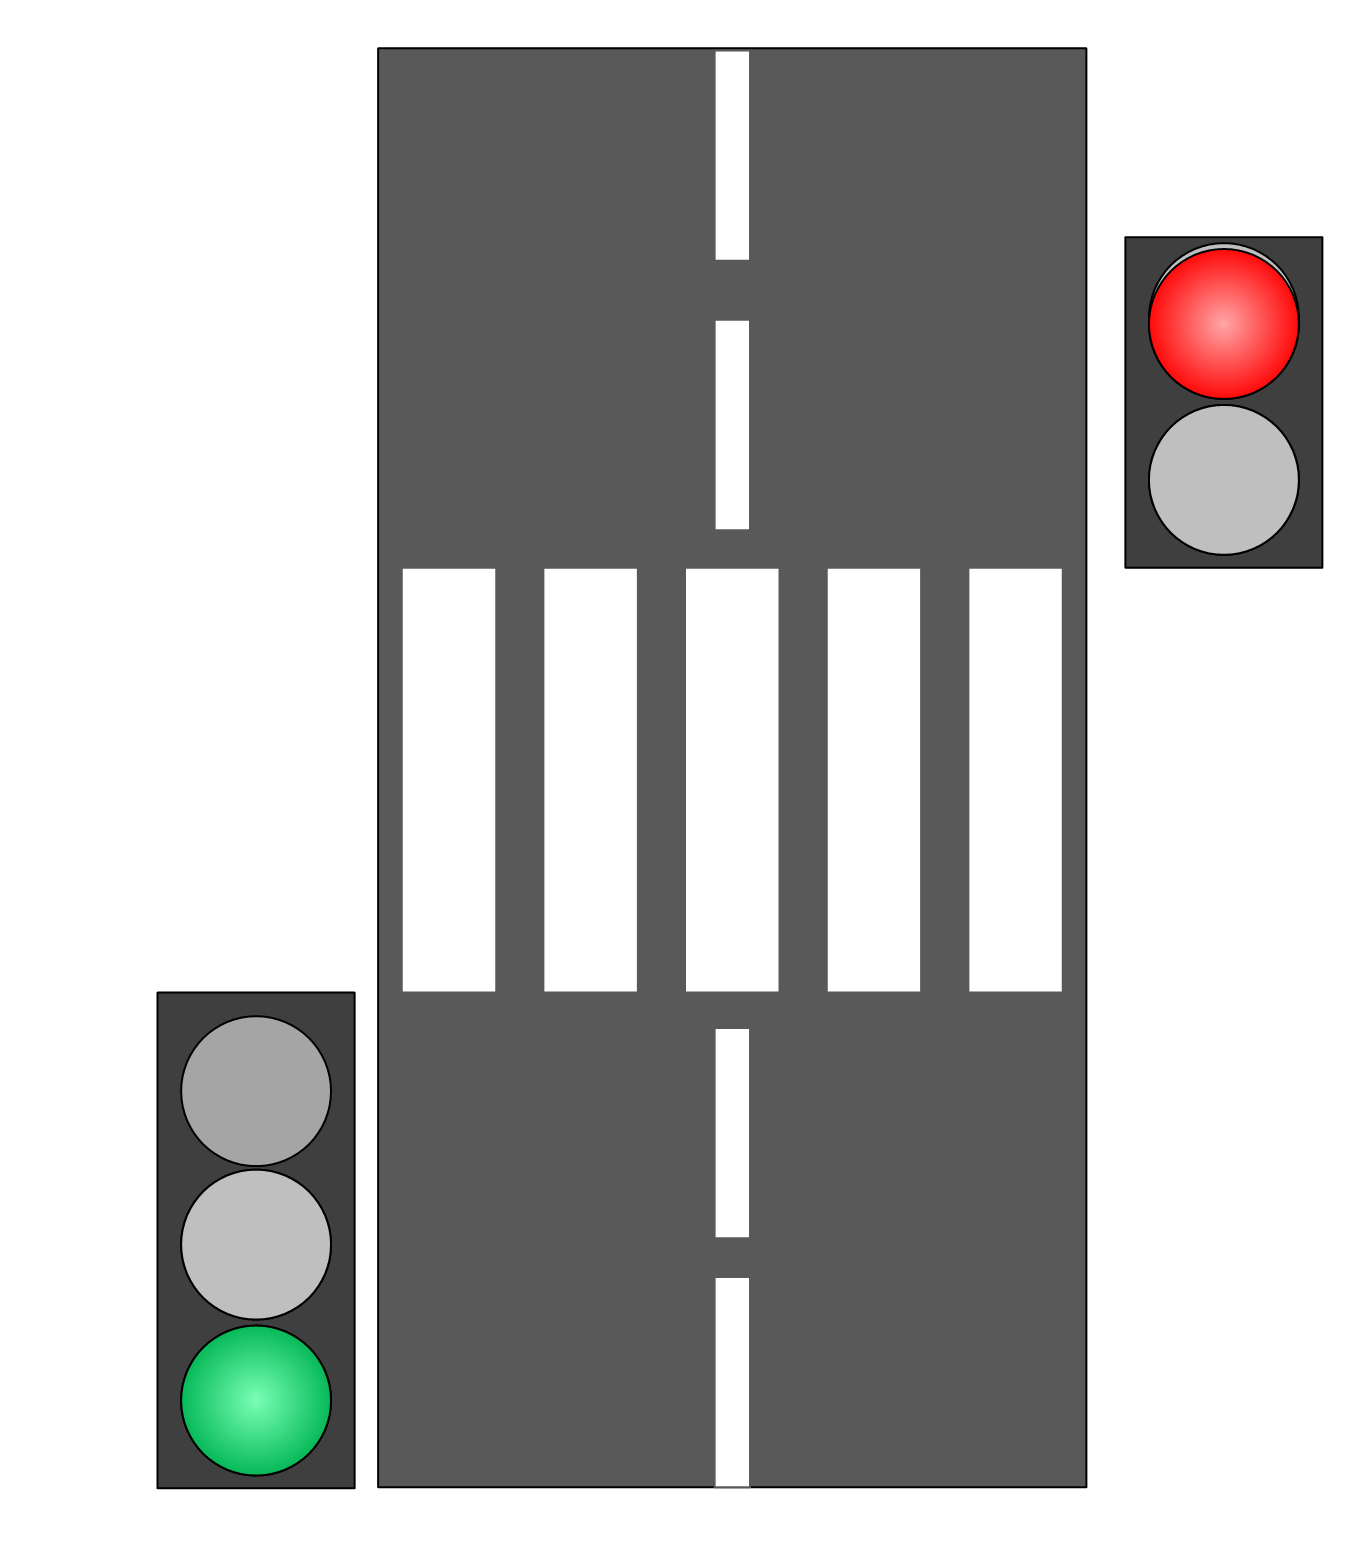
\includegraphics[width=30mm, keepaspectratio]{figures/casestudy_state1.png}
	}
	\fbox{
		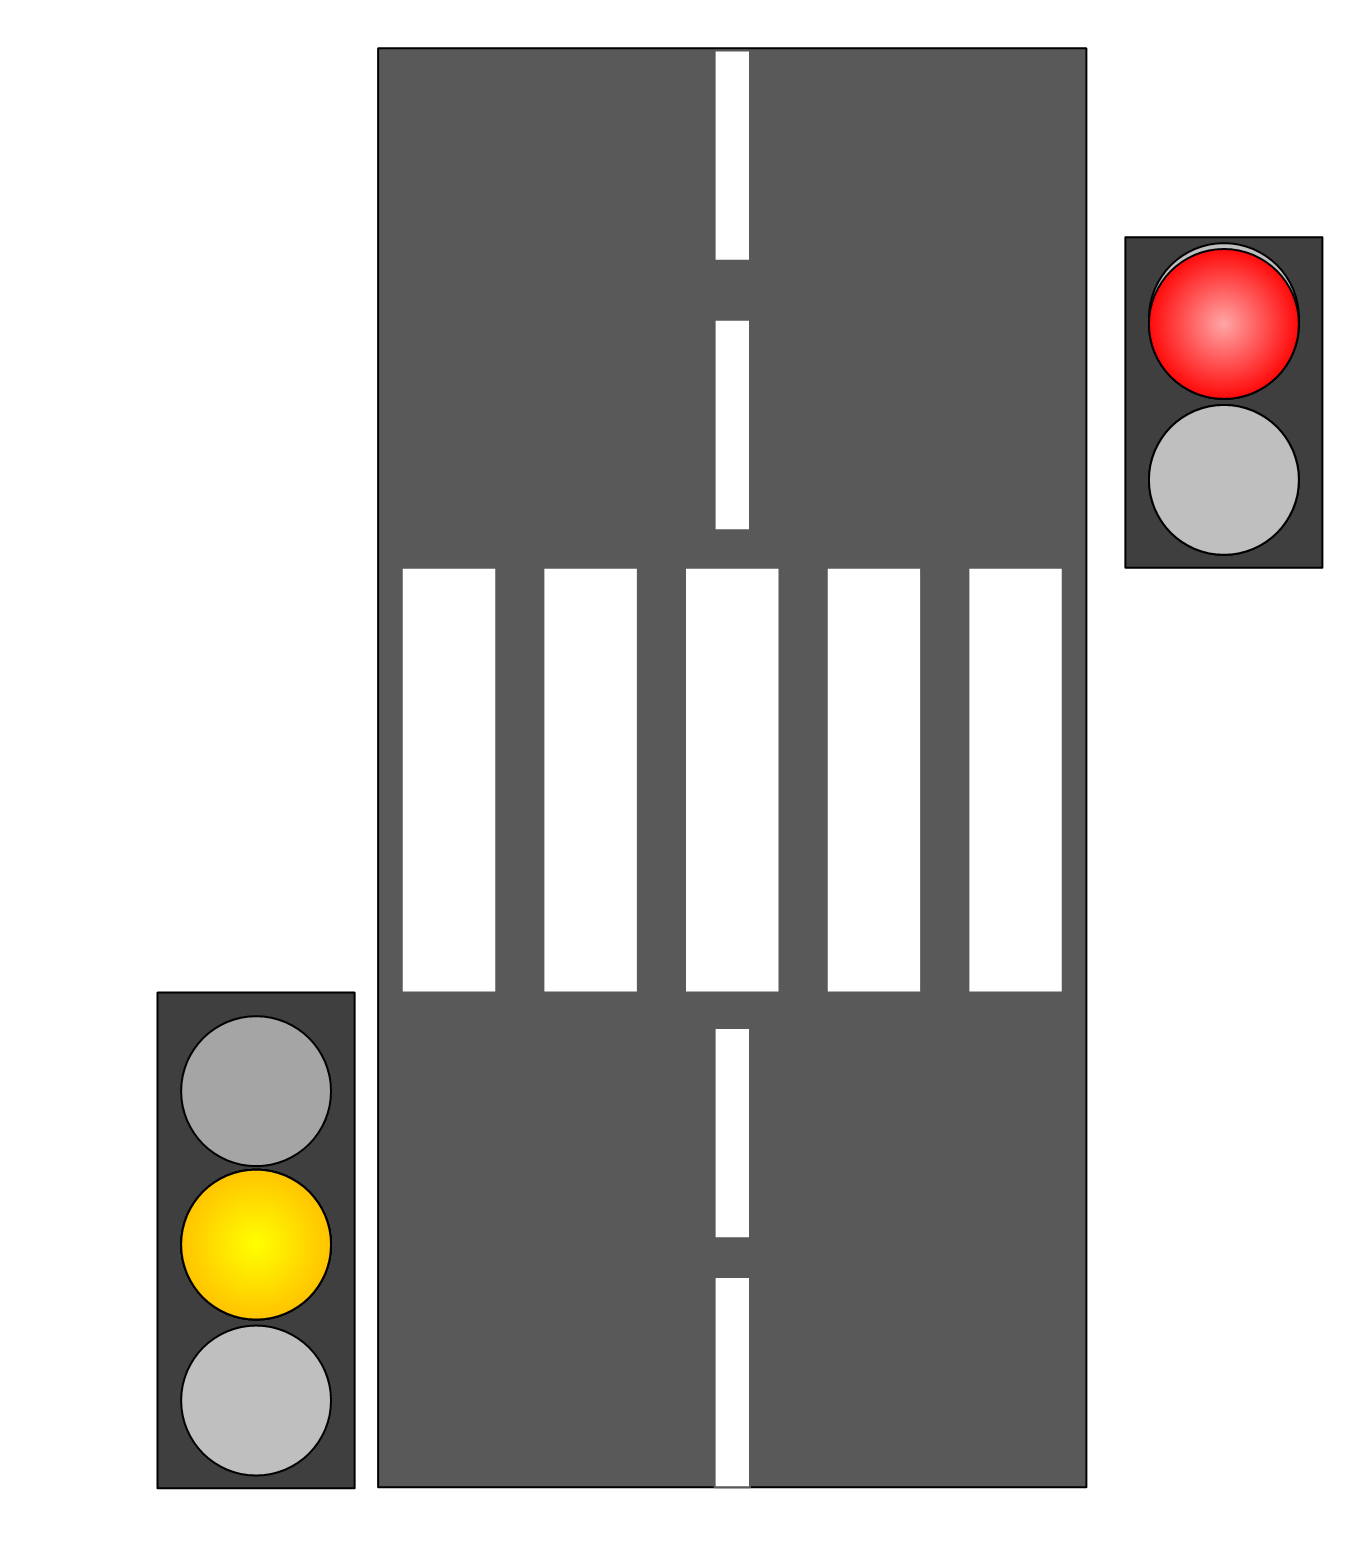
\includegraphics[width=30mm, keepaspectratio]{figures/casestudy_state2.png}
	}
	\fbox{
		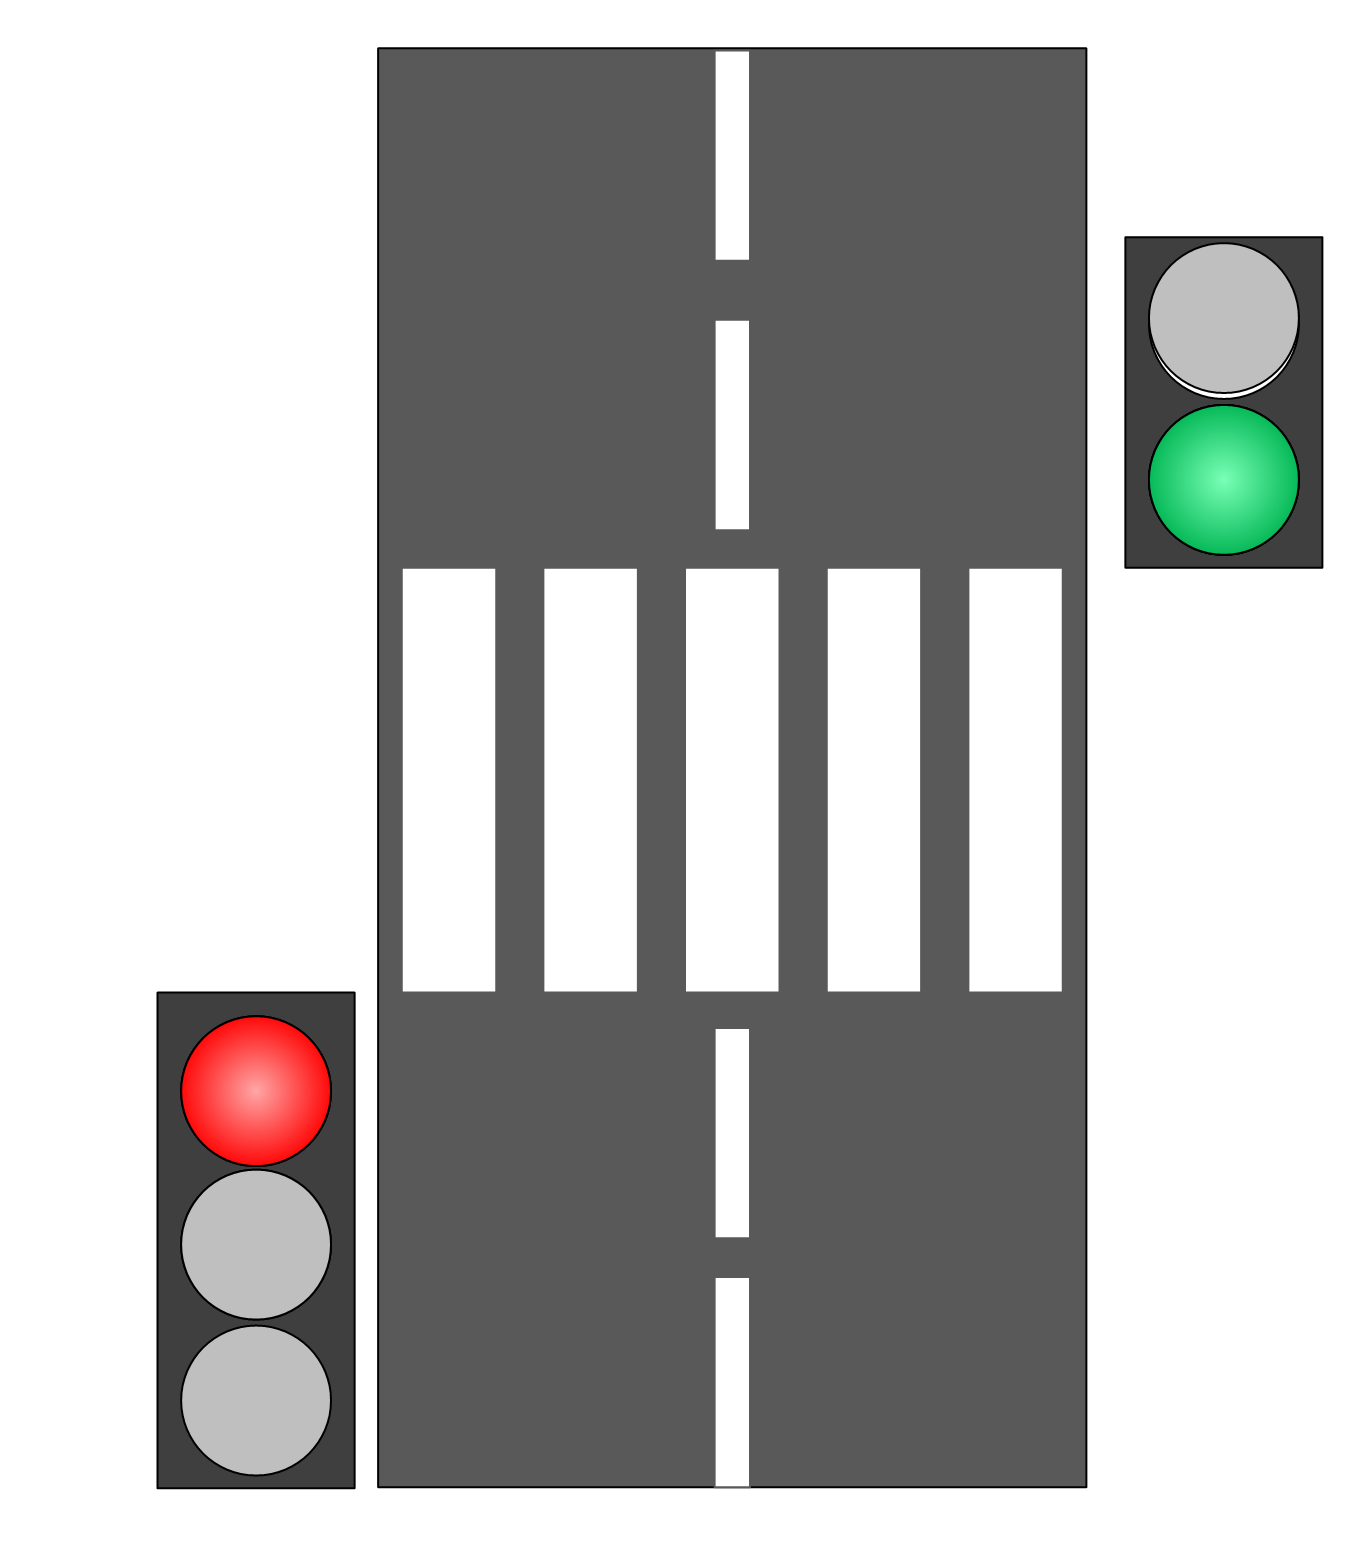
\includegraphics[width=30mm, keepaspectratio]{figures/casestudy_state3.png}
	}
	\fbox{
		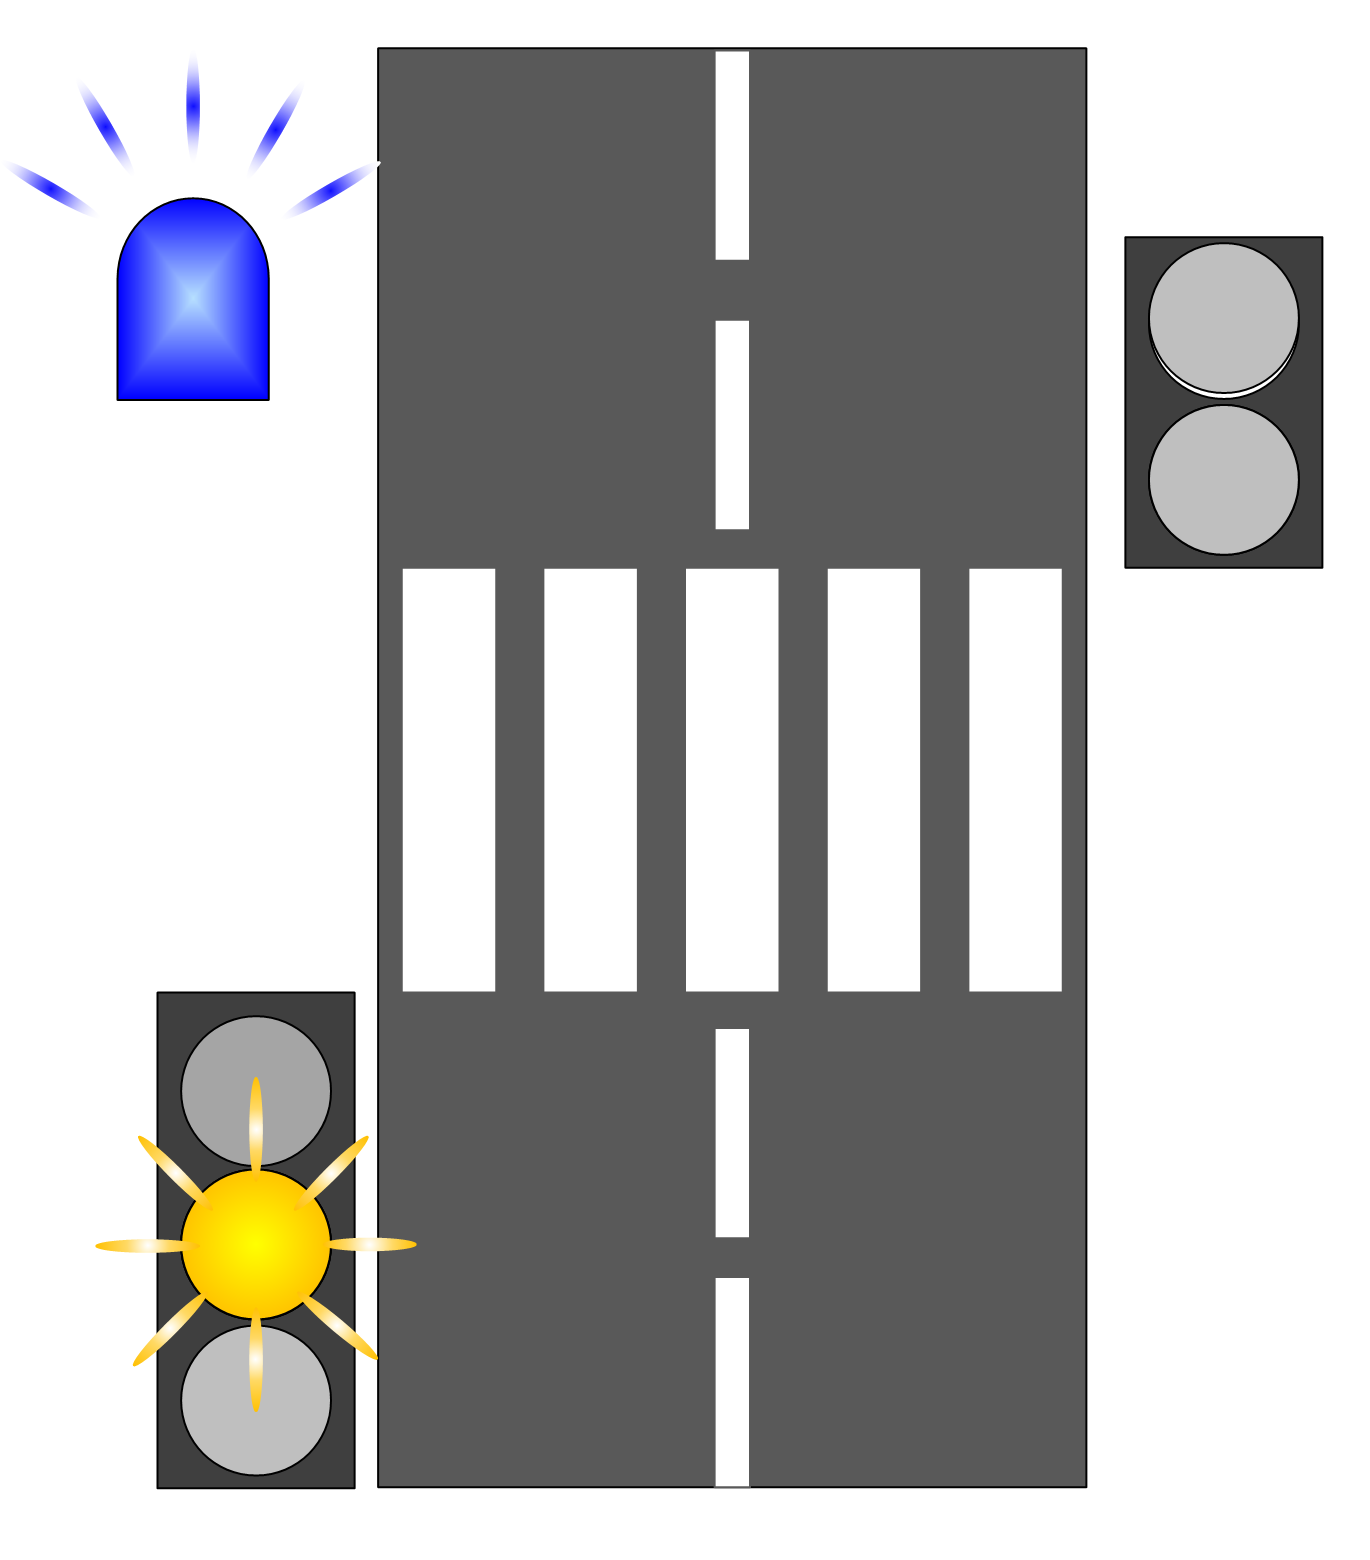
\includegraphics[width=30mm, keepaspectratio]{figures/casestudy_state4.png}
	}
	\caption{Possible states of the system: normal operation (\textit{three from the left}) and the interrupted state \textit{(right)}} 
	\label{fig_casestudy_systemstates}
\end{figure}

%---------------------------------------------------------------
\subsection{Component Design} \label{subs_casestudycomps}
%---------------------------------------------------------------

The previous subsection mentioned two components of the composite system: a traffic light and a pedestrian light. To realize the safe state of the system, the components must synchronize their behavior, justificating the existence of a third, controller component. The traffic and pedestrian light components should have one input and one output port -- they  are relatively simple -- and the controller should have an input port for the police and two output ports for the components.

\textbf{The traffic light component} has two possible inputs on its input port (TrafficControl) - toggle and interrupt - and four outputs on its output port (TrafficDisplay) - red, green, yellow and blinking yellow - as it appeared in the problem description.

\textbf{The pedestrian light component} has the same two inputs on its input port (PedestrianControl) - toggle and interrupt - and three outputs on its output port (PedestrianDisplay) - red, green, and black - as it appeared in the problem description.

\textbf{The controller component} controls the rhythm of the change of states and also interrupts the other components when the police interrupt arrives. It has an input port ('\textit{Police}') for the police interrupt and two output ports ('\textit{TrafficControl}' and '\textit{PedestrianControl}') - matching the input ports of the other components.

The described components and their connections are illustrated on Figure \ref{fig_casestudy_blockdiagram}.

\begin{figure}[!ht] 
	\centering
	%\fbox{
		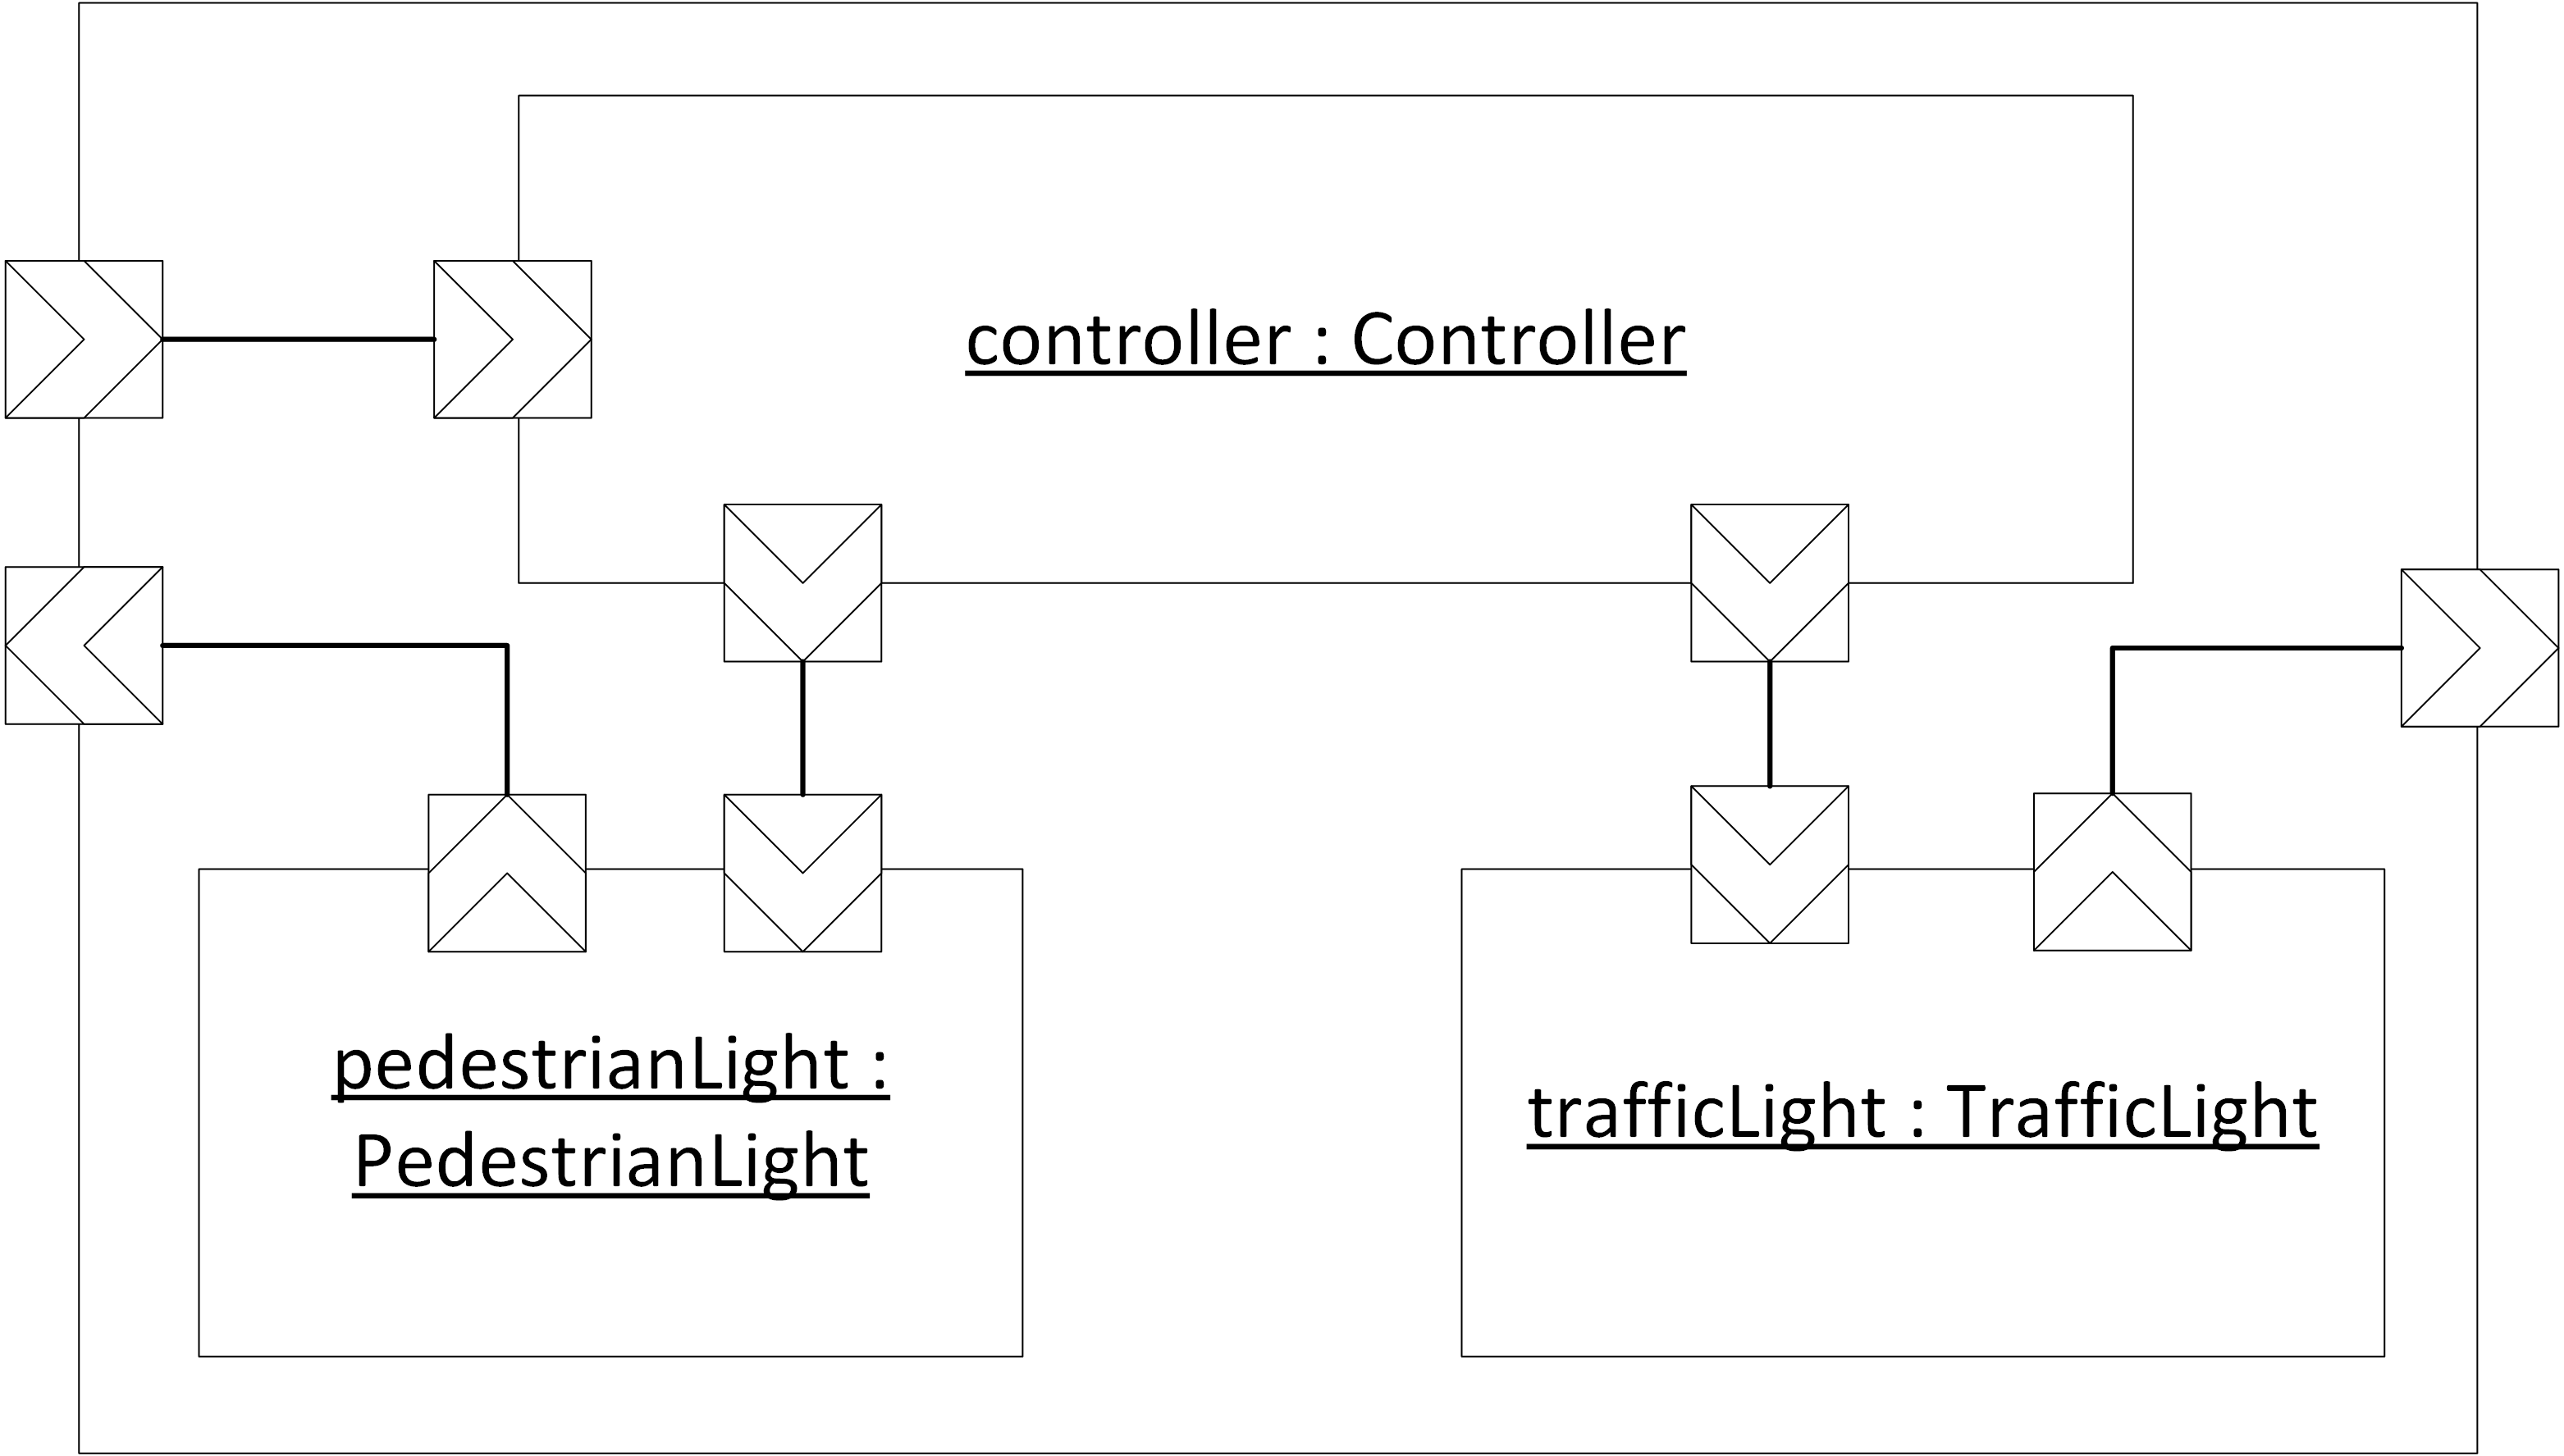
\includegraphics[width=130mm, keepaspectratio]{figures/casestudy_blockdiagram.png}
	%}
	\caption{Components of the modeled system and their connections} 
	\label{fig_casestudy_blockdiagram}
\end{figure}

\textbf{The Expected Behavior of the Components} 

The components have been separated and their interfaces precisely defined, thus, we can proceed to formulating behavior-related requirements. For instance, the traffic light component must conform to the following -- not exhaustive -- list:

\begin{itemize}
	\item The traffic light must loop through the sequence 'toggle/red toggle/green toggle/yellow toggle/red' during normal operation.
	\item The traffic light must display blinking yellow signal when a police interrupt arrives during normal operation.
	\item The traffic light must return to normal operation when a second interrupt arrives.
	\item The traffic light must display red signal when returning to normal operation.
	\item The traffic light must always display blinking yellow when interrupted. 

\end{itemize}

A very similar list can be constructed for the pedestrian light component. The controller component is slightly more complicated, as it may toggle or interrupt the other components at the same time, so its alphabet shall contain separate elements for these cases.

%---------------------------------------------------------------
\subsection{Synthesizing the Components} \label{subs_casestudysynth}
%---------------------------------------------------------------

Now we add the previously formulated requirements to the ILE, in formalisms that it is able to interpret. In the following examples for the interaction of the user with the ILE, '$\circ$' symbolizes the ILE and '$\triangleright$' symbolizes the user (interface qualifications are omitted for shorter and simpler expressions). 

\bigskip
\fbox{
	\parbox{\textwidth}{
		\begin{itemize}
			\setlength\itemsep{0.2em}
			\item[$\circ$] Provide the requirements for component 'TrafficLight':
			\item[$\triangleright$] Valid Trace: toggle/red toggle/green toggle/yellow toggle/red
			\item[$\triangleright$] LTL Expression: F(interrupt -> X(G(toggle) -> G(blinkingYellow)))
			\item[$\triangleright$] Invalid Trace: interrupt/red interrupt/blinkingYellow
			\item[$\triangleright$] LTL Expression: F(G(interrupt -> (blinkingYellow | red)))
			
			\smallskip
			... other components ...
		\end{itemize}
	}
}

\bigskip
After adding these requirements during the offline phase, the synthesis of the components can proceed to the online, interactive phase. A possible run of the learning process can be seen below.

\bigskip
\fbox{
	\parbox{\textwidth}{
		\begin{itemize}
			\setlength\itemsep{0.2em}
			\item[$\circ$] Learning component 'TrafficLight'
			\item[$\circ$] Provide the output for sequence [toggle, interrupt]:
			\item[$\triangleright$] Corresponding Output: blinkingYellow
			\item[$\circ$] Provide the output for sequence [toggle, interrupt, interrupt]:
			\item[$\triangleright$] Corresponding Output: red
			\item[$\circ$] Provide the output for sequence [toggle, toggle, interrupt]:
			\item[$\triangleright$] Corresponding Output: blinkingYellow
			\item[$\circ$] Provide the output for sequence [toggle, toggle, interrupt, interrupt]:
			\item[$\triangleright$] Corresponding Output: red
			\item[$\circ$] Provide the output for sequence [toggle, toggle, toggle, interrupt]:
			\item[$\triangleright$] Corresponding Output: blinkingYellow
			\item[$\circ$] Equivalence Query (Figure \ref{fig_trafficlightincomplete} in the Appendix)
			\item[$\triangleright$] Counterexample: interrupt interrupt
			\item[$\circ$] Provide the output for sequence [interrupt, interrupt, interrupt]:
			\item[$\triangleright$] Valid Trace: interrupt/blinkingYellow interrupt/red interrupt/blinkingYellow interrupt/red
			\item[$\circ$] Provide the output for sequence [interrupt, interrupt, toggle]:
			\item[$\triangleright$] Corresponding Output: green
			\item[$\circ$] Provide the output for sequence [interrupt, toggle, interrupt]:
			\item[$\triangleright$] Corresponding Output: red
			\item[$\circ$] Equivalence Query (Figure \ref{fig_casestudy_trafficlightlearned})
			\item[$\triangleright$] Approved.
			
			\smallskip
			... other components ...
		\end{itemize}
	}
}

\bigskip
The same learning process can be seen on Listing \ref{lst_examplelearning} in the Appendix, which presents the inputs and outputs as they appeara on the command line interface.

%---------------------------------------------------------------
\subsection{The Learned Models} \label{subs_casestudyresults}
%---------------------------------------------------------------

Now we can examine any differences between the expected and the learned models. Figure \ref{fig_casestudy_trafficlightdiff} presents the expected and the synthesized traffic light models.

\begin{figure}[!ht] 
	\centering
	\begin{subfigure}[b]{0.9\textwidth}
		\centering
		\fbox{
			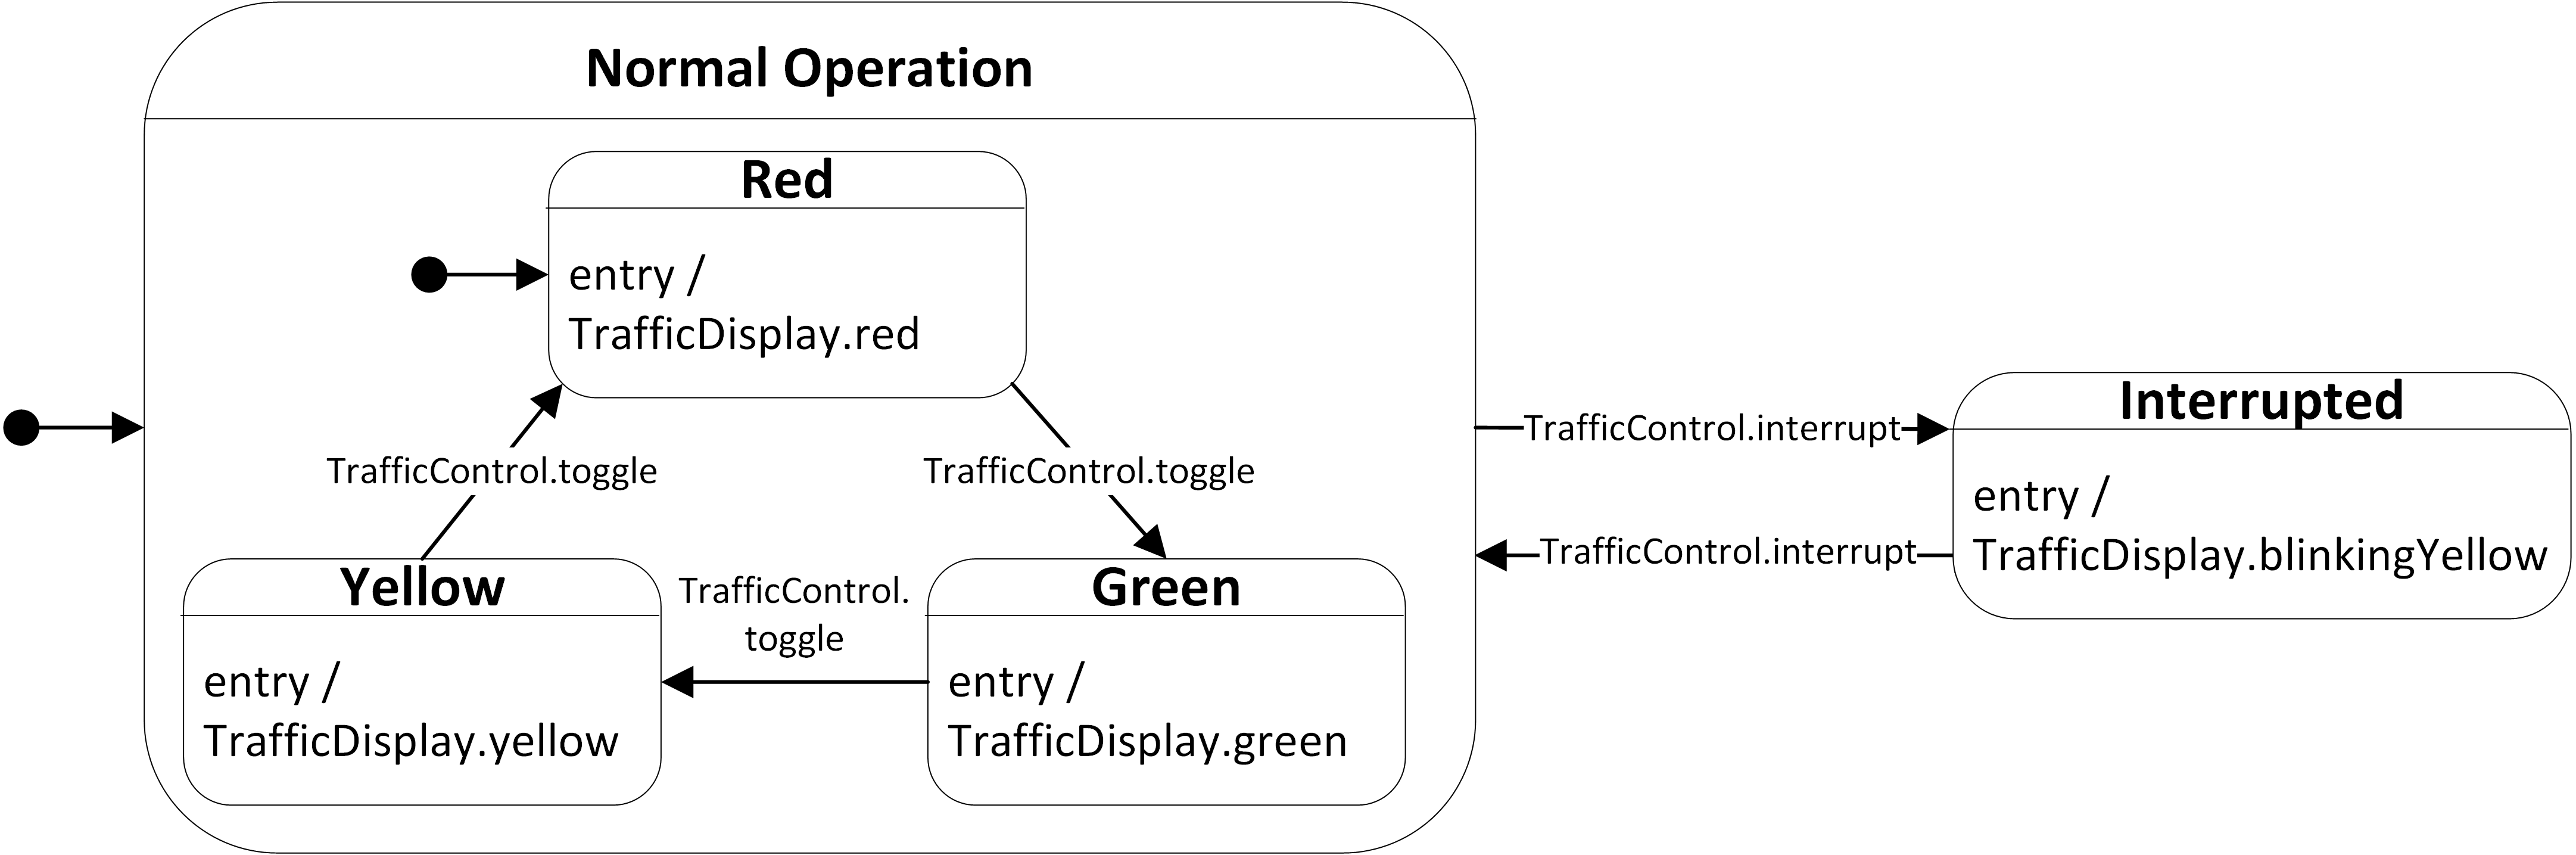
\includegraphics[width=120mm]{figures/casestudy_trafficlightexpected.png}
		}	
		\caption{Expected}
	\end{subfigure}
	\hfill
	\begin{subfigure}[b]{0.9\textwidth}
		\centering
		\fbox{
			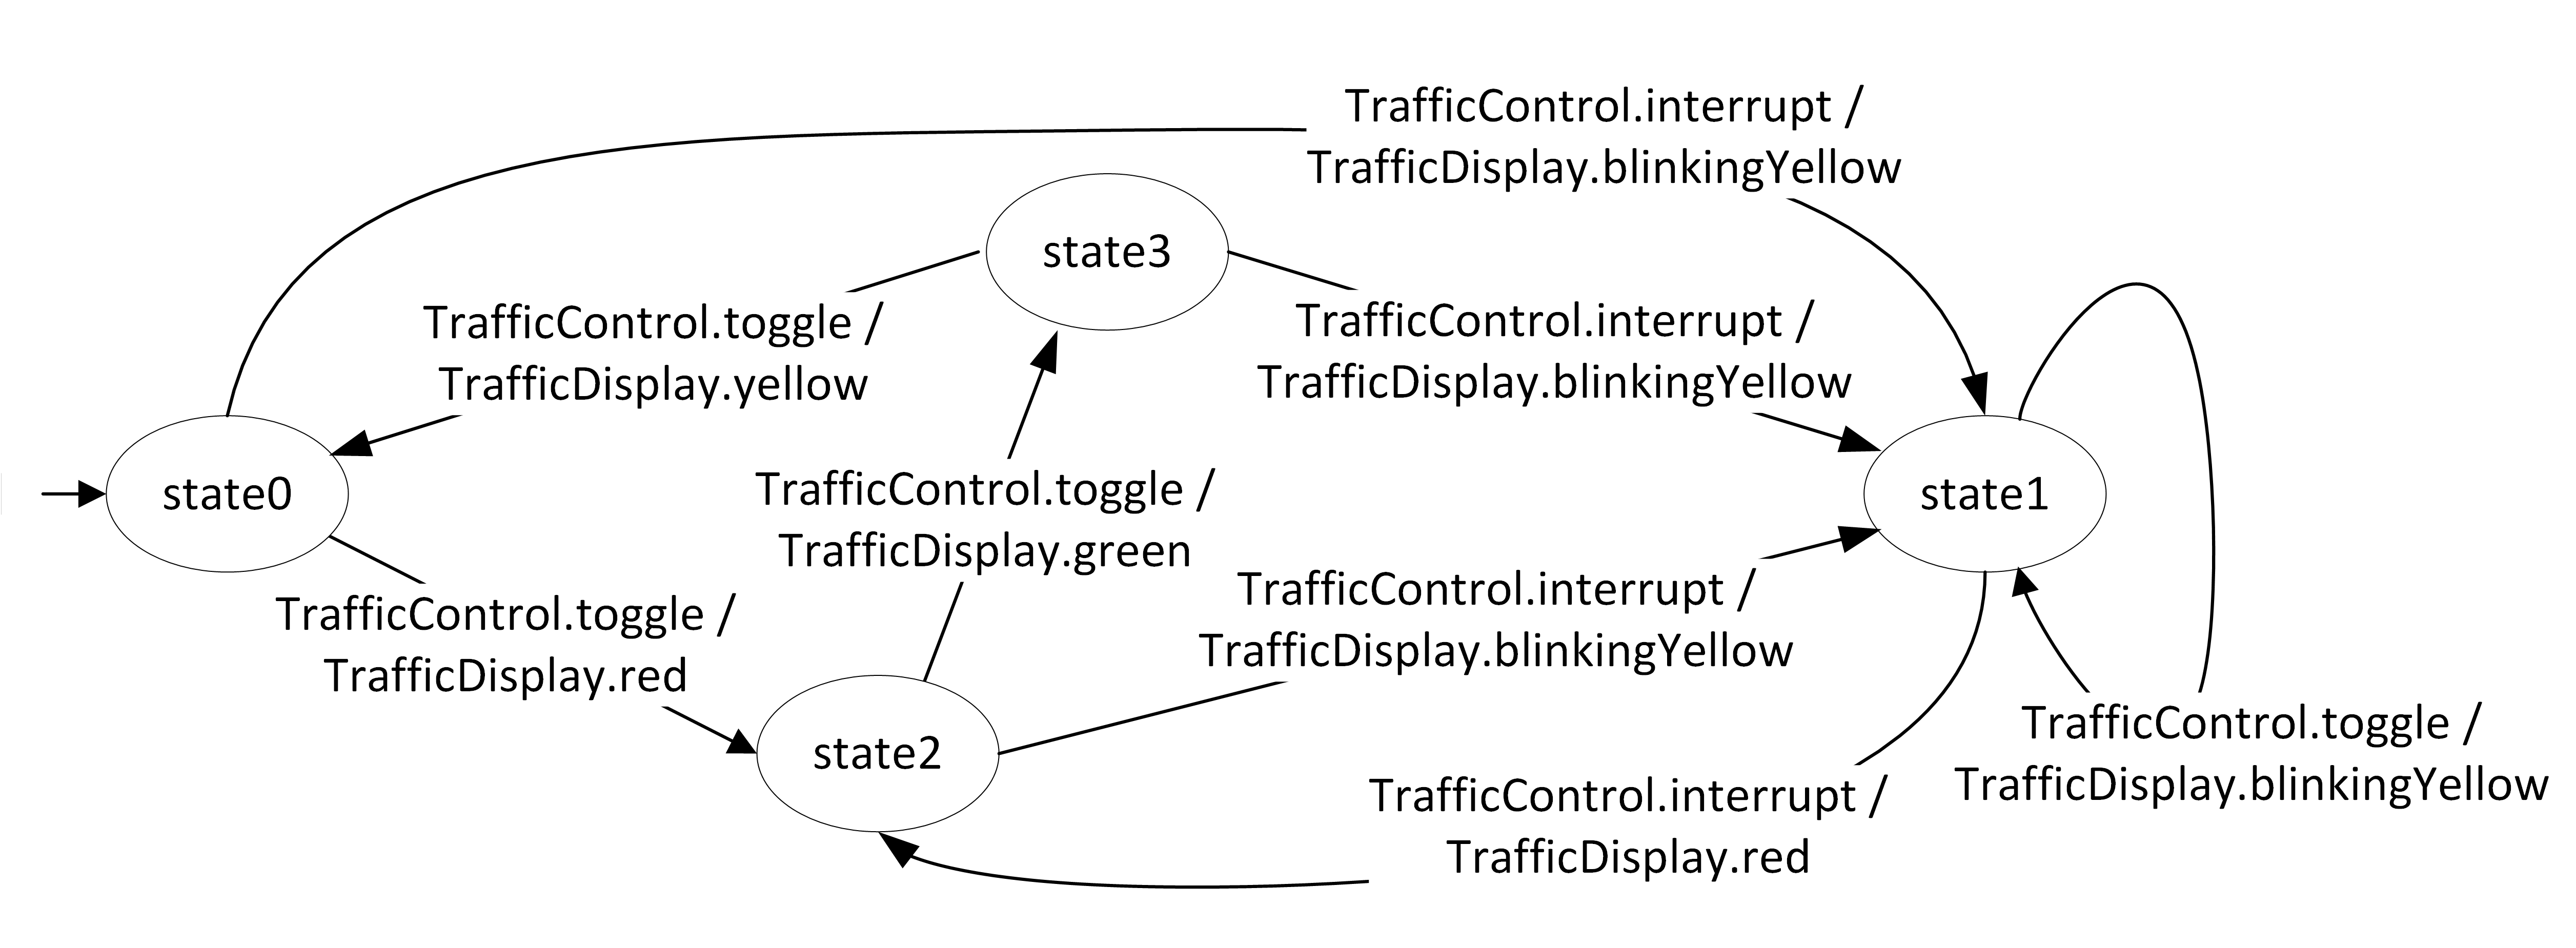
\includegraphics[width=120mm]{figures/casestudy_trafficlightlearned.png}
		}
		\caption{Learned}	
		\label{fig_casestudy_trafficlightlearned}
	\end{subfigure}
	\caption{The expected and the learned traffic light components}
	\label{fig_casestudy_trafficlightdiff}
\end{figure}

The structure of the models is clearly different, notably:
\begin{itemize}
	\item The expected models contain hierarchical states, while the learned ones are 'flat'.
	\item The expected models also contain entry and exit actions, while the learned models only contain actions on transitions. 
	\item The expected models contain meaningful state names, while the learned ones only have generated ones.
\end{itemize}

However, the models are behaviorally equivalent. Both models meet the requirements stated in Subsection \ref{subs_casestudycomps}, and after careful examination, it is obvious that the only initial states are different -- as no entry actions are used in the learned models -- and the transition starting from the hierarchical state is separated into three different transitions.

The differences between the expected and learned pedestrian light components can be seen on Figure \ref{fig_casestudy_pedestrianlightdiff}. The differences are the similar to those of the traffic light models, as the modeled behavior is also very similar. 

\begin{figure}[!ht] 
	\centering
	\begin{subfigure}[b]{0.9\textwidth}
		\centering
		\fbox{
			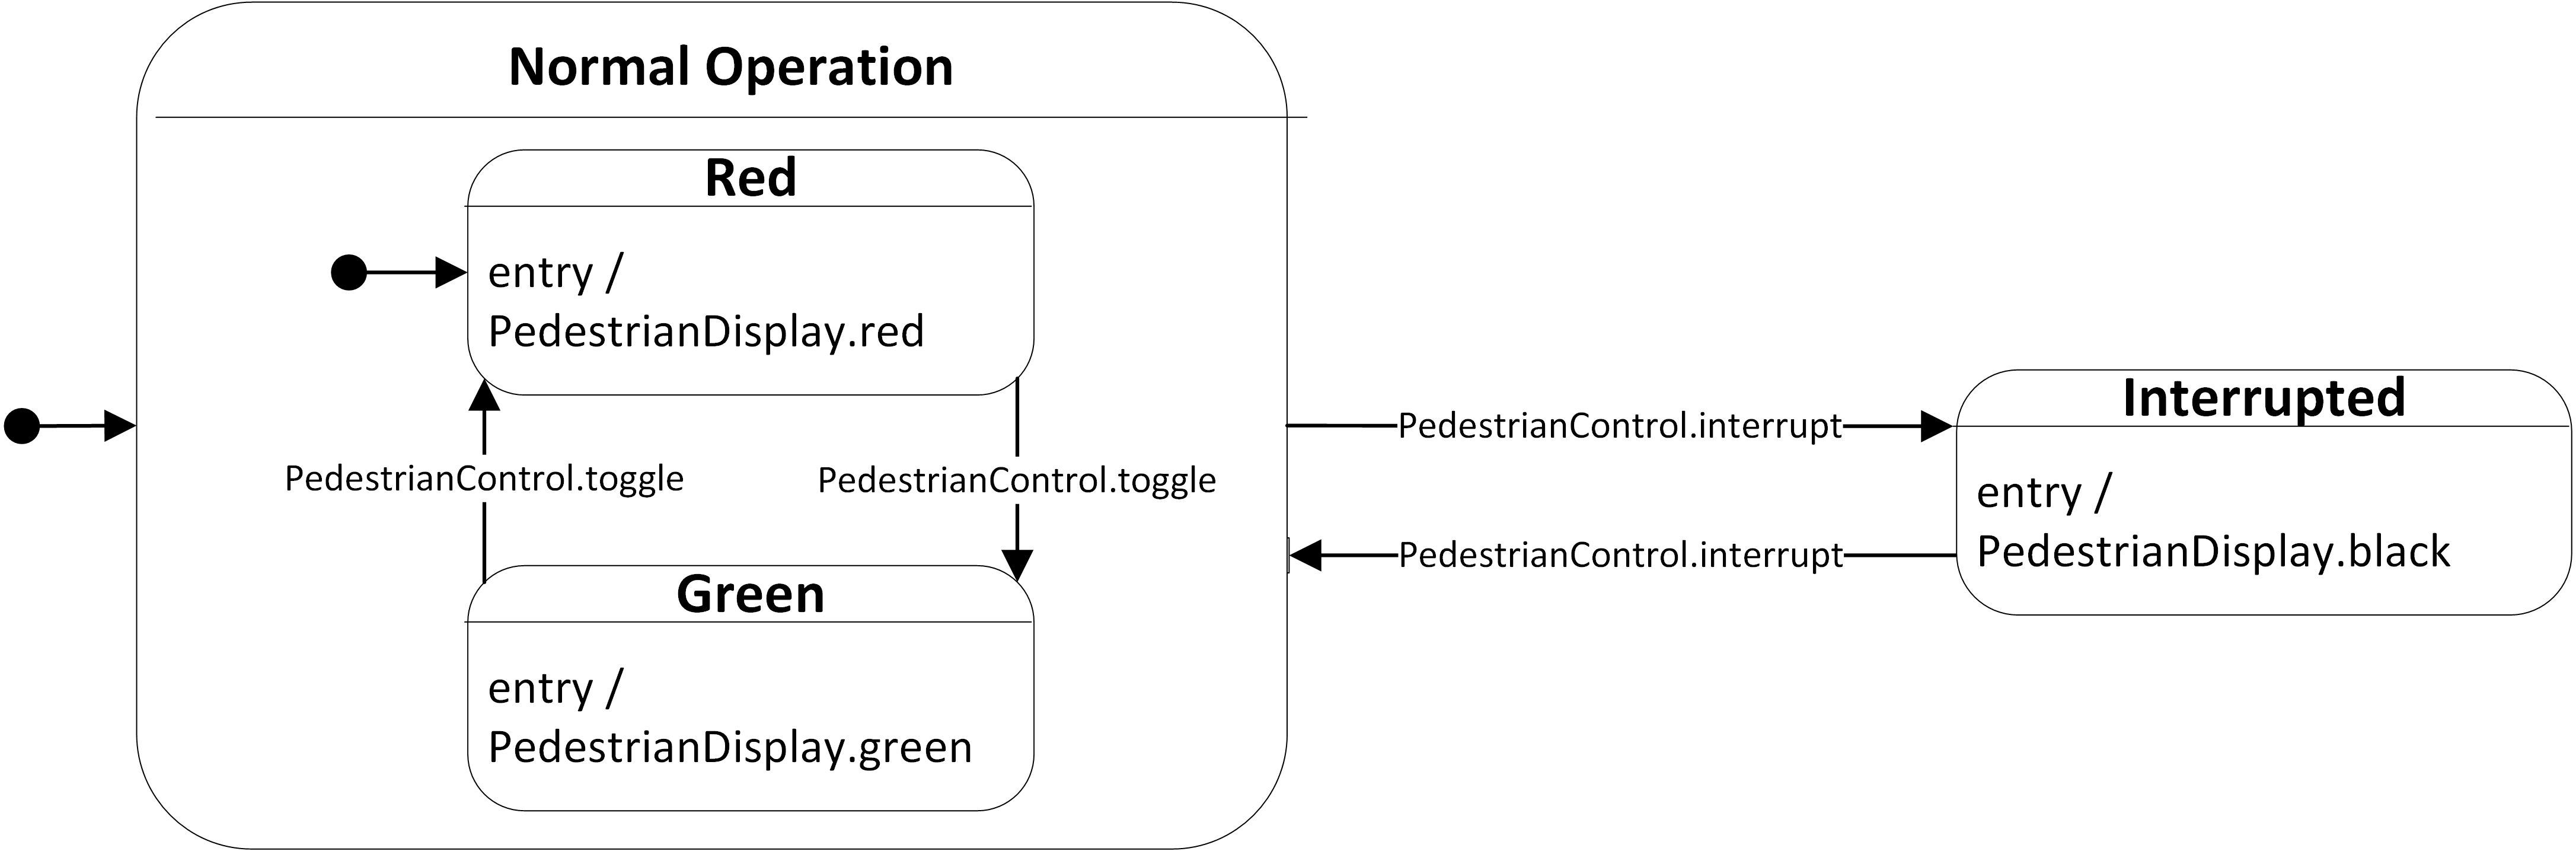
\includegraphics[width=120mm]{figures/casestudy_pedestrianlightexpected.png}
		}	
		\caption{Expected}
	\end{subfigure}
	\hfill
	\begin{subfigure}[b]{0.9\textwidth}
		\centering
		\fbox{
			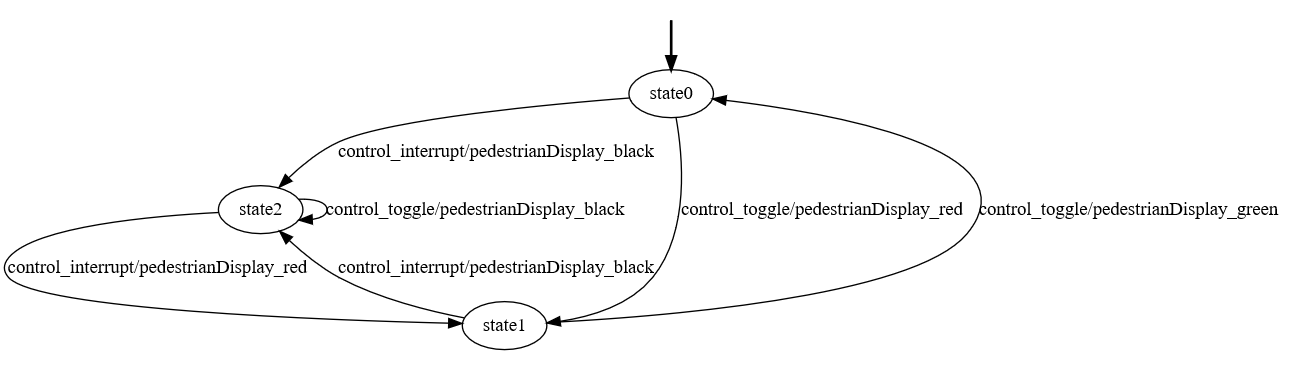
\includegraphics[width=120mm]{figures/casestudy_pedestrianlightlearned.PNG}
		}
		\caption{Learned}	
	\end{subfigure}
	\caption{The expected and the learned pedestrian light components}
	\label{fig_casestudy_pedestrianlightdiff}
\end{figure}

The behavior of the controller component can be learned similarly. The expected and the synthesized models can be seen on Figure \ref{fig_casestudy_controllerdiff}. Note, that in addition to '{\fontfamily{qcr}\selectfont Police.interrupt}', the component also has an unqualified t input word. This represents a timeout event the engineer must extend the serialized model with -- but acts as a regular input event during the learning. 

\begin{figure}[!ht] 
	\centering
	\begin{subfigure}[b]{0.9\textwidth}
		\centering
		\fbox{
			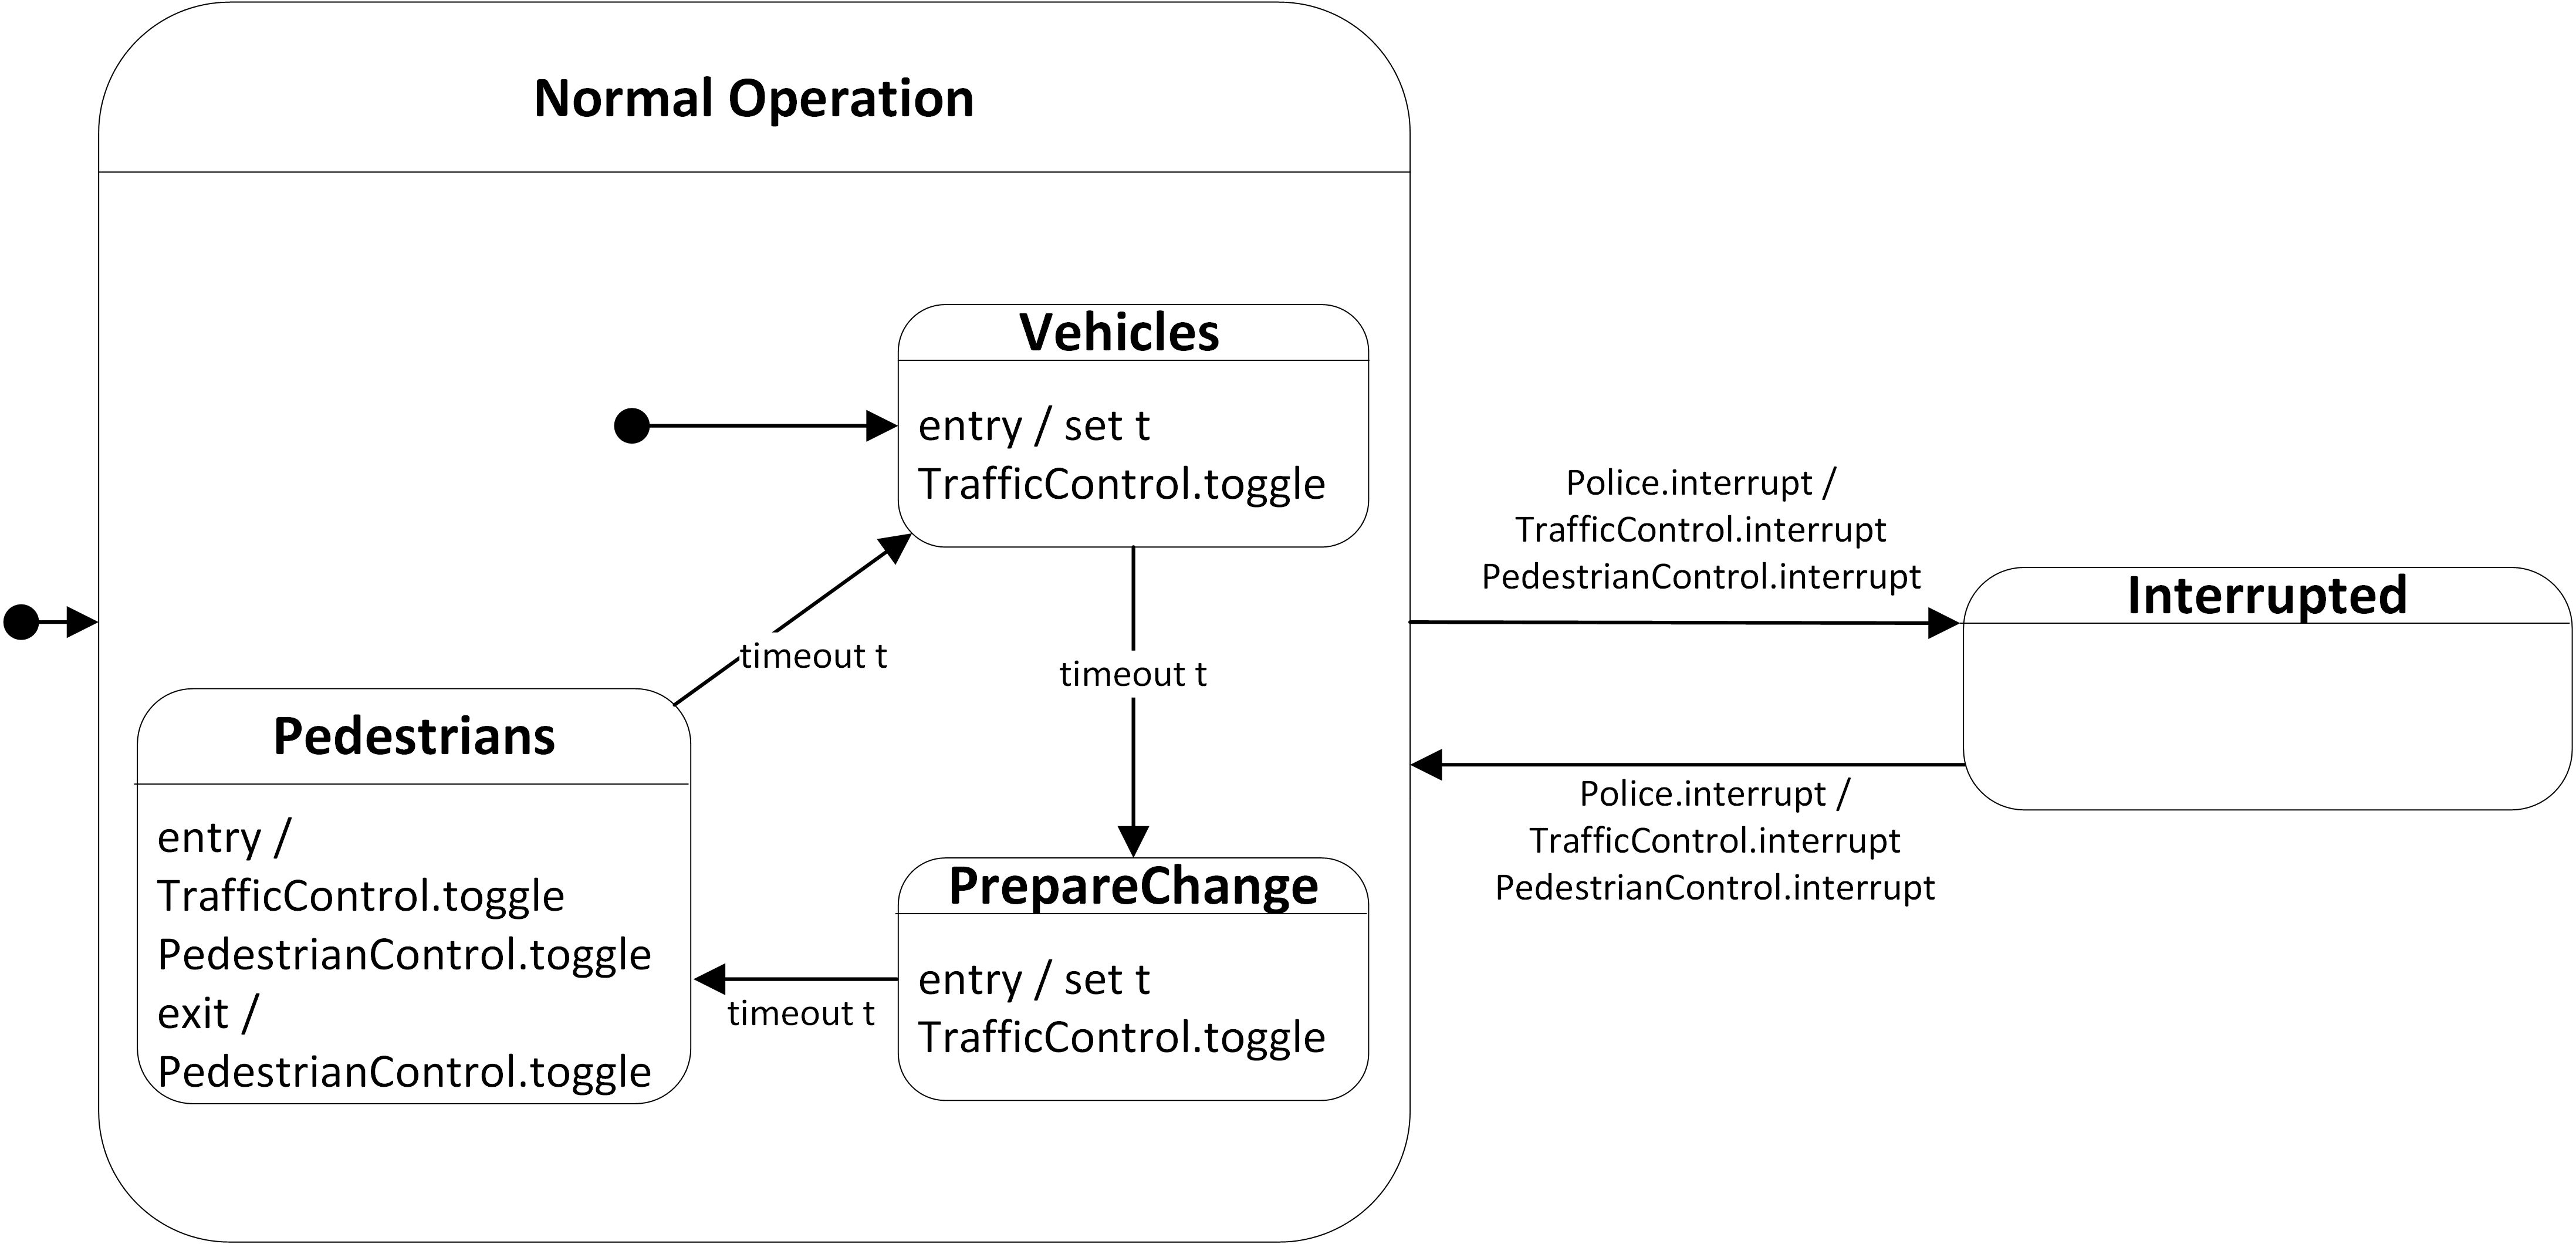
\includegraphics[width=120mm]{figures/casestudy_controllerexpected.png}
		}	
		\caption{Expected}
	\end{subfigure}
	\hfill
	\begin{subfigure}[b]{0.9\textwidth}
		\centering
		\fbox{
			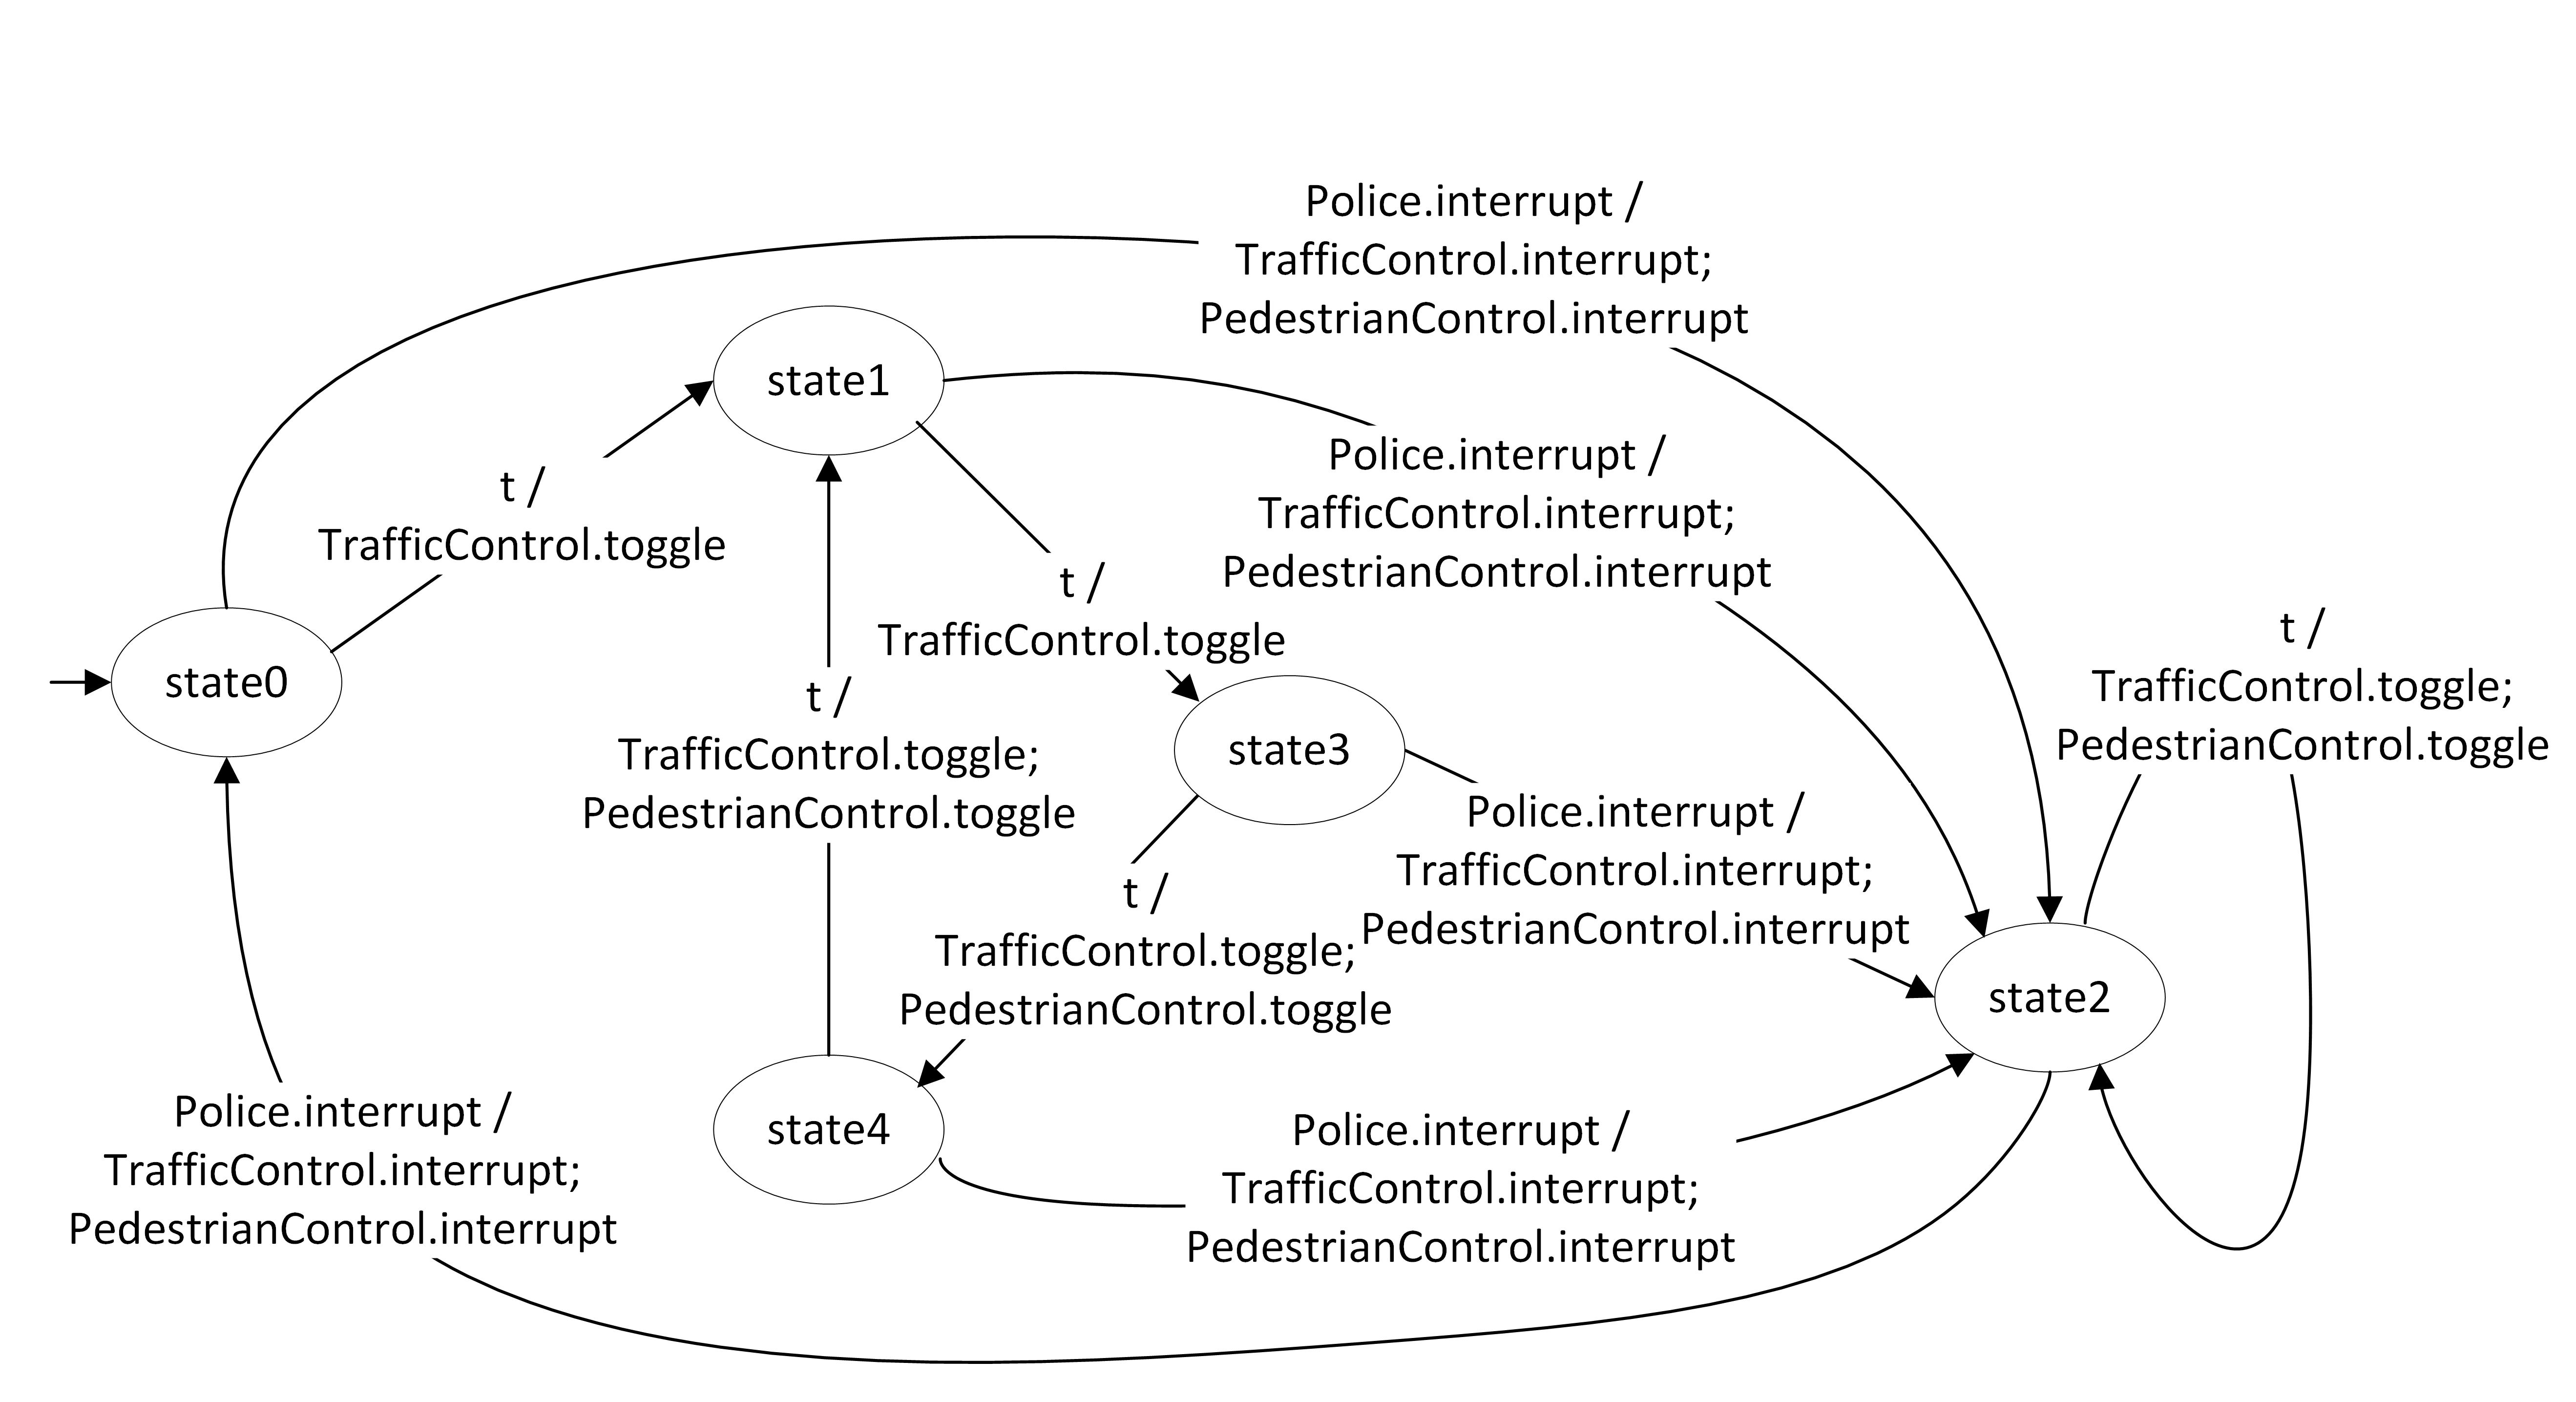
\includegraphics[width=120mm]{figures/casestudy_controllerlearned.png}
		}
		\caption{Learned [TODO ezt szebbre]}	
	\end{subfigure}
	\caption{The expected and the learned controller components}
	\label{fig_casestudy_controllerdiff}
\end{figure}

After learning every component, the collection of the models is serialized as a Gamma project, with the following files and contents:
\begin{itemize}
	\item TrafficLight.gcd (the learned traffic light component)
	\item PedestrianLight.gcd (the learned pedestrian light component)
	\item Controller.gcd (the learned controller component)
	\item CompositeSystem.gcd (connections between the component ports, as illustrated on Figure \ref{fig_casestudy_blockdiagram})
	\item Interfaces.gcd (the interface definitions based on the ports of the components)
\end{itemize}
After extending the controller with statechart-specific elements (namely the timeout event), the engineer can use the Gamma Framework to check the correctness of the system model or even generate implementation code.


[TODO ESETLEG: a teljes rendszert is tanuljuk?]

\clearpage
%----------------------------------------------------------------------------
\section{Theoretical Evaluation} \label{sec_theoeval}
%----------------------------------------------------------------------------
%TODO: Bevezető

%---------------------------------------------------------------
\subsection{The Oracle} \label{subs_evaloracle}
%---------------------------------------------------------------
%TODO: Optimistic vs Pessimistic, formalizmusok
The main metric of the oracle is the number of questions the engineer has to answer during the course of the model synthesis. This is really difficult to measure, as the exact number of these questions depends on multiple parameters: the complexity of the desired model, as well as the order, formalism, complexity and skillful construction of the requirements formulated by the designing engineer. Some of these parameters is difficult to measure in itself, thus, the following measurement is rather an illustration of the capabilities of the framework through a realistic example. 

For this, the traffic light component from the case study in Section \ref{sec_casestudy} is going to be used. We assume, that the user only adds requirements he perceives conducive to the model synthesis and tries to formulate realistic -- not unnecessarily complex -- requirements. 

The baseline of this experiment is the number of questions the user has to answer by always providing the corresponding outputs to the questions of the ILE, as higher numbers are the result of unnecessary information. Then, we are going to examine the cases when valid traces are also allowed, then add LTL expressions and finally invalid traces. Sequence diagrams are excluded from these measurements. The results can be seen on Figure \ref{fig_eval_trafficlightformalisms}.

\begin{figure}[!ht] 
	\centering
	%\fbox{
	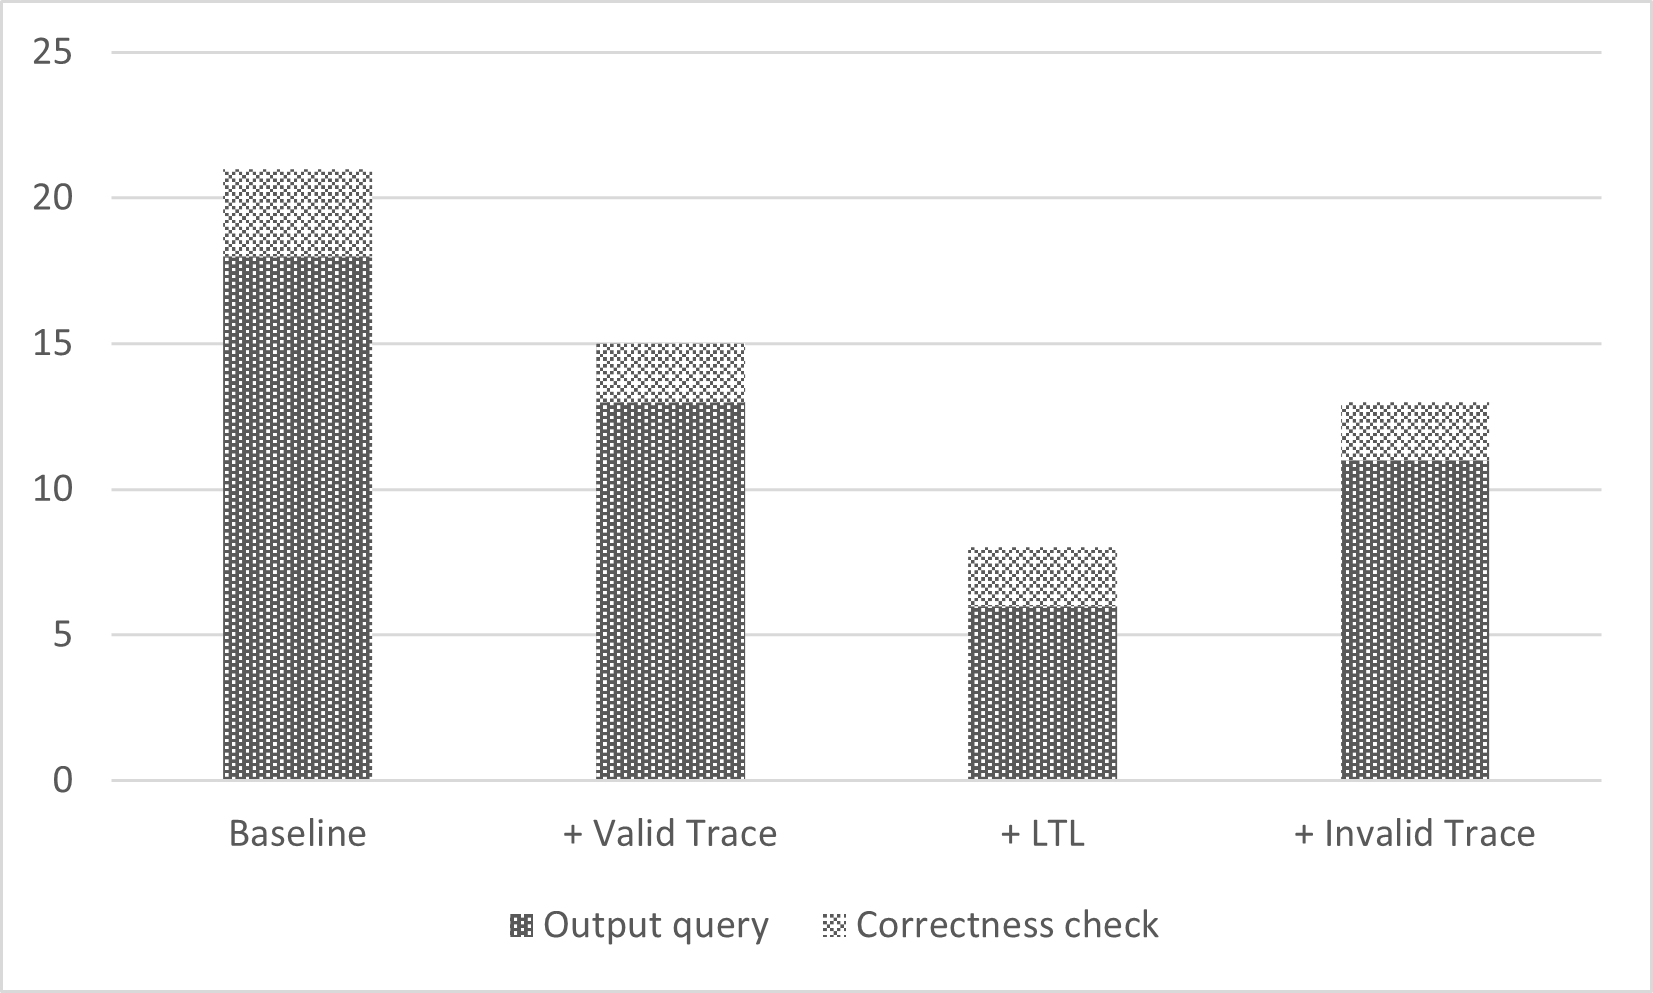
\includegraphics[width=130mm, keepaspectratio]{figures/evaluation_trafficlightformalism.png}
	%}
	\caption{Components of the modeled system and their connections} 
	\label{fig_eval_trafficlightformalisms}
\end{figure}

The requirements used in this experiment -- apart from the corresponding outputs answering the questions of the ILE directly -- can be seen in [TODO appendix]. The smallest number of queries was measured when both valid traces and LTL expressions were used. The addition of invalid traces resulted in a slightly higher number, demonstrating that this formalism is difficult to apply and useful mostly for its other benefits.  
 
%---------------------------------------------------------------
\subsection{The Learning Algorithm} \label{subs_evallearningalgo}
%---------------------------------------------------------------
%TODO: Optimistic vs Pessimistic, minimization

%---------------------------------------------------------------
\subsection{Caching} \label{subs_evalcaching}
%---------------------------------------------------------------
%TODO: optimisticre mennyit csökkent, RESET
%----------------------------------------------------------------------------
\chapter{Conclusion} \label{conclusion}
%----------------------------------------------------------------------------
%%----------------------------------------------------------------------------
\chapter{\LaTeX-eszközök}
\label{sec:LatexTools}
%----------------------------------------------------------------------------
\section{A szerkesztéshez használatos eszközök}
%----------------------------------------------------------------------------
Ez a sablon TeXstudio 2.8.8 szerkesztővel készült. A TeXstudio egy platformfüggetlen, Windows, Linux és Mac OS alatt is elérhető \LaTeX-szerkesztőprogram számtalan hasznos szolgáltatással (\refstruc{fig:TeXstudio}). A szoftver ingyenesen letölthető\footnote{A TeXstudio hivatalos oldala: \url{http://texstudio.sourceforge.net/}}.

\begin{figure}[!ht]
\centering
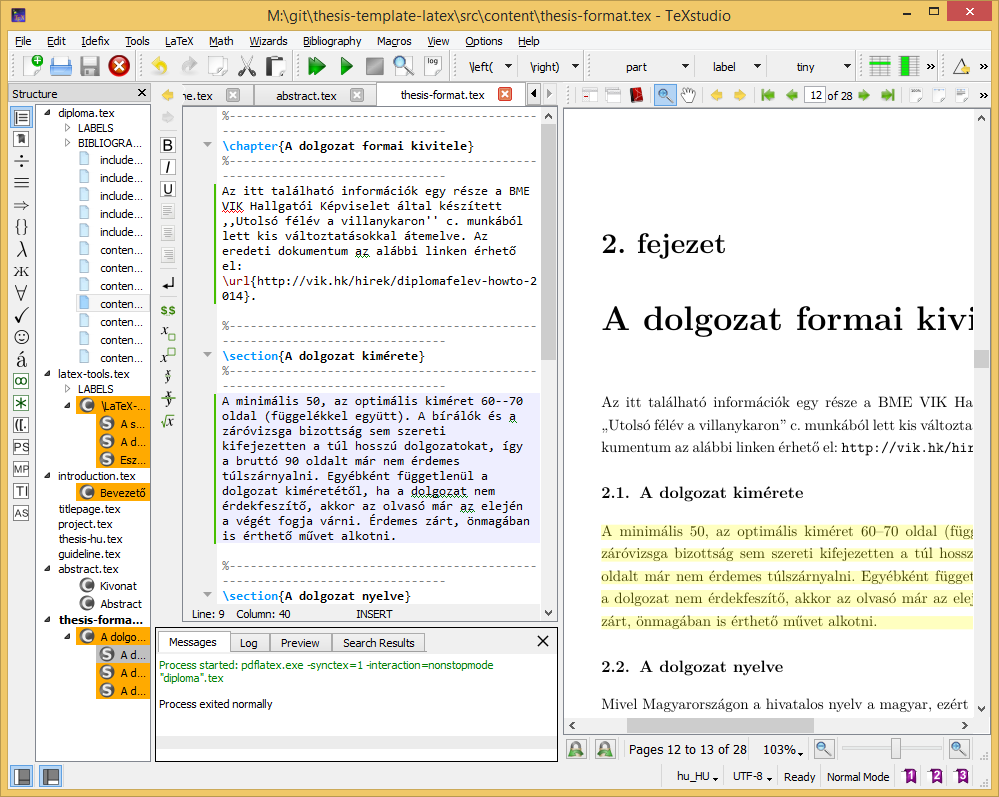
\includegraphics[width=150mm, keepaspectratio]{figures/TeXstudio.png}
\caption{A TeXstudio \LaTeX-szerkesztő.}
\label{fig:TeXstudio}
\end{figure}

A TeXstudio telepítése után érdemes még letölteni a magyar nyelvű helyesírásellenőrző-szótárakat hozzá. A TeXstudio az OpenOffice-hoz használatos formátumot tudja kezelni. A TeXstudio beállításainál a \verb+General+ fülön a \verb+Dictionaries+ résznél tudjuk megadni, hogy melyik szótárat használja.

Egy másik használható Windows alapú szerkesztőprogram a LEd\footnote{A LEd hivatalos oldala: \url{http://www.latexeditor.org/}} (LaTeX Editor), a TeXstudio azonban stabilabb, gyorsabb, és jobban használható.

%----------------------------------------------------------------------------
\section{A dokumentum lefordítása Windows alatt}
%----------------------------------------------------------------------------
A TeXstudio és a LEd kizárólag szerkesztőprogram (bár az utóbbiban DVI-nézegető is van), így a dokumentum fordításához szükséges eszközöket nem tartalmazza. Windows alatt alapvetően két lehetőség közül érdemes választani: MiKTeX (\url{http://miktex.org/}) és TeX Live (\url{http://www.tug.org/texlive/}) programcsomag. Az utóbbi működik Mac OS X, GNU/Linux alatt és Unix-származékokon is. A MiKTeX egy alapcsomag telepítése után mindig letölti a használt funkciókhoz szükséges, de lokálisan hiányzó \TeX-csomagokat, míg a TeX Live DVD ISO verzóban férhető hozzá. Ez a dokumentum TeX Live 2008 programcsomag segítségével fordult, amelynek DVD ISO verziója a megadott oldalról letölthető. A sablon lefordításához a disztribúcióban szereplő \verb+magyar.ldf+ fájlt a \verb+http://www.math.bme.hu/latex/+ változatra kell cserélni, vagy az utóbbi változatot be kell másolni a projekt-könyvtárba (ahogy ezt meg is tettük a sablonban) különben anomáliák tapasztalhatók a dokumentumban (pl. az ábra- és táblázat-aláírások formátuma nem a beállított lesz, vagy bizonyos oldalakon megjelenik alapértelmezésben egy fejléc). A TeX Live 2008-at még nem kell külön telepíteni a gépre, elegendő DVD-ről (vagy az ISO fájlból közvetlenül, pl. DaemonTools-szal) használni.

Ha a MiKTeX csomagot használjuk, akkor parancssorból a következő módon tudjuk újrafordítani a teljes dokumentumot:

\begin{lstlisting}[language=bash,frame=single,float=!ht]
$ texify -p thesis.tex
\end{lstlisting}

A \verb+texify+ parancs a MiKTex programcsomag \verb+miktex/bin+ alkönyvtárában található. A parancs gondoskodik arról, hogy a szükséges lépéseket (fordítás, hivatkozások generálása stb.) a megfelelő sorrendben elvégezze. A \verb+-p+ kapcsoló hatására PDF-et generál. A fordítást és az ideiglenes fájlok törlését elvégezhetjük a sablonhoz mellékelt \verb+manual_build.bat+ szkript segítségével is.

A \TeX-eszközöket tartalmazó programcsomag binárisainak elérési útját gyakran be kell állítani a szerkesztőprogramban, például TeXstudio esetén legegyszerűbben az \verb+Options / Configure TeXstudio... / Commands+ menüponttal előhívott dialógusablakban tehetjük ezt meg.

A PDF-\LaTeX~használata esetén a generált dokumentum közvetlenül PDF-formátumban áll rendelkezésre. Amennyiben a PDF-fájl egy PDF-nézőben (pl. Adobe Acrobat Reader vagy Foxit PDF Reader) meg van nyitva, akkor a fájlleírót a PDF-néző program tipikusan lefoglalja. Ilyen esetben a dokumentum újrafordítása hibaüzenettel kilép. Ha bezárjuk és újra megnyitjuk a PDF dokumentumot, akkor pedig a PDF-nézők többsége az első oldalon nyitja meg a dokumentumot, nem a legutóbb olvasott oldalon. Ezzel szemben például az egyszerű és ingyenes \textcolor{blue}{Sumatra PDF} nevű program képes arra, hogy a megnyitott dokumentum megváltozását detektálja, és frissítse a nézetet az aktuális oldal megtartásával.

%----------------------------------------------------------------------------
\section{Eszközök Linuxhoz}
%----------------------------------------------------------------------------
Linux operációs rendszer alatt is rengeteg szerkesztőprogram van, pl. a KDE alapú Kile jól használható. Ez ingyenesen letölthető, vagy éppenséggel az adott Linux-disztribúció eleve tartalmazza, ahogyan a dokumentum fordításához szükséges csomagokat is. Az Ubuntu Linux disztribúciók alatt például legtöbbször a \verb+texlive-*+ csomagok telepítésével használhatók a \LaTeX-eszközök. A jelen sablon fordításához szükséges csomagok (kb. 0,5 GB) az alábbi paranccsal telepíthetők:

\begin{lstlisting}[language=bash,morekeywords={sudo,apt\-get},alsoletter={-},breaklines=true]
$ sudo apt-get install texlive-latex-extra texlive-fonts-extra texlive-fonts-recommended texlive-lang-european texlive-xetex texlive-science
\end{lstlisting}

Amennyiben egy újabb csomag hozzáadása után hiányzó fájlra utaló hibát kapunk a fordítótól, telepítenünk kell az azt tartalmazó TeX Live csomagot. Ha pl. a \verb+bibentry+ csomagot szeretnénk használni, futtassuk az alábbi parancsot:

\begin{lstlisting}[language=bash,morekeywords={apt\-cache},alsoletter={-},breaklines=true]
$ apt-cache search bibentry
texlive-luatex - TeX Live: LuaTeX packages
\end{lstlisting}

Majd telepítsük fel a megfelelő TeX Live csomagot, jelen esetben a `texlive-lualatex`-et. (Egy LaTeX csomag több TeX Live csomagban is szerepelhet.)

Ha gyakran szerkesztünk más \LaTeX dokumentumokat is, kényelmes és biztos megoldás a teljes TeX Live disztribúció telepítése, ez azonban kb. 4 GB helyet igényel.

\begin{lstlisting}[language=bash,morekeywords={sudo,apt\-get},alsoletter={-},breaklines=true]
sudo apt-get install texlive-full
\end{lstlisting}

%%----------------------------------------------------------------------------
\chapter{A dolgozat formai kivitele}
%----------------------------------------------------------------------------
Az itt található információk egy része a BME VIK Hallgatói Képviselet által készített ,,Utolsó félév a villanykaron'' c. munkából lett kis változtatásokkal átemelve. Az eredeti dokumentum az alábbi linken érhető el: \url{http://vik.hk/hirek/diplomafelev-howto-2015}.

%----------------------------------------------------------------------------
\section{A dolgozat kimérete}
%----------------------------------------------------------------------------
Szakdolgozat esetében minimum 30, 45 körüli ajánlott oldalszám lehet az iránymutató. De mindenképp érdemes rákérdezni a konzulensnél is az elvárásokra, mert tanszékenként változóak lehetnek az elvárások.

Mesterképzésen a Diplomatervezés 1 esetében a beszámoló még inkább az Önálló laboratóriumi beszámolókhoz hasonlít, tanszékenként eltérő formai követelményekkel, -- egy legalább 30 oldal körüli dolgozat az elvárt -- és az elmúlt fél éves munkáról szól. De egyben célszerű, ha ez a végleges diplomaterv alapja is. (A végleges 60-90 oldal körülbelül a hasznos részre nézve)


%----------------------------------------------------------------------------
\section{A dolgozat nyelve}
%----------------------------------------------------------------------------
Mivel Magyarországon a hivatalos nyelv a magyar, ezért alapértelmezésben magyarul kell megírni a dolgozatot. Aki külföldi posztgraduális képzésben akar részt venni, nemzetközi szintű tudományos kutatást szeretne végezni, vagy multinacionális cégnél akar elhelyezkedni, annak célszerű angolul megírnia diplomadolgozatát. Mielőtt a hallgató az angol nyelvű verzió mellett dönt, erősen ajánlott mérlegelni, hogy ez mennyi többletmunkát fog a hallgatónak jelenteni fogalmazás és nyelvhelyesség terén, valamint -- nem utolsó sorban -- hogy ez mennyi többletmunkát fog jelenteni a konzulens illetve bíráló számára. Egy nehezen olvasható, netalán érthetetlen szöveg teher minden játékos számára.

%----------------------------------------------------------------------------
\section{A dokumentum nyomdatechnikai kivitele}
%----------------------------------------------------------------------------
A dolgozatot A4-es fehér lapra nyomtatva, 2,5 centiméteres margóval (+1~cm kötésbeni), 11--12 pontos betűmérettel, talpas betűtípussal és másfeles sorközzel célszerű elkészíteni.

Annak érdekében, hogy a dolgozat külsőleg is igényes munka benyomását keltse, érdemes figyelni az alapvető tipográfiai szabályok betartására~\cite{Jeney}.

%% !TeX spellcheck = hu_HU
% !TeX encoding = UTF-8
% !TeX program = xelatex
%----------------------------------------------------------------------------
\chapter{A \LaTeX-sablon használata}
%----------------------------------------------------------------------------

Ebben a fejezetben röviden, implicit módon bemutatjuk a sablon használatának módját, ami azt jelenti, hogy sablon használata ennek a dokumentumnak a forráskódját tanulmányozva válik teljesen világossá. Amennyiben a szoftver-keretrendszer telepítve van, a sablon alkalmazása és a dolgozat szerkesztése \LaTeX-ben a sablon segítségével tapasztalataink szerint jóval hatékonyabb, mint egy WYSWYG (\emph{What You See is What You Get}) típusú szövegszerkesztő esetén (pl. Microsoft Word, OpenOffice).

%----------------------------------------------------------------------------
\section{Címkék és hivatkozások}
%----------------------------------------------------------------------------
A \LaTeX~dokumentumban címkéket (\verb+\label+) rendelhetünk ábrákhoz, táblázatokhoz, fejezetekhez, listákhoz, képletekhez stb. Ezekre a dokumentum bármely részében hivatkozhatunk, a hivatkozások automatikusan feloldásra kerülnek.

A sablonban makrókat definiáltunk a hivatkozások megkönnyítéséhez. Ennek megfelelően minden ábra (\emph{figure}) címkéje \verb+fig:+ kulcsszóval kezdődik, míg minden táblázat (\emph{table}), képlet (\emph{equation}), fejezet (\emph{section}) és lista (\emph{listing}) rendre a \verb+tab:+, \verb+eq:+, \verb+sec:+ és \verb+lst:+ kulcsszóval kezdődik, és a kulcsszavak után tetszőlegesen választott címke használható. Ha ezt a konvenciót betartjuk, akkor az előbbi objektumok számára rendre a \verb+\figref+, \verb+\tabref+, \verb+\eqref+, \verb+\sectref+ és \verb+\listref+ makrókkal hivatkozhatunk. A makrók paramétere a címke, amelyre hivatkozunk (a kulcsszó nélkül). Az összes említett hivatkozástípus, beleértve az \verb+\url+ kulcsszóval bevezetett web-hivatkozásokat is a  \verb+hyperref+\footnote{Segítségével a dokumentumban megjelenő hivatkozások nem csak dinamikussá válnak, de színezhetők is, bővebbet erről a csomag dokumentációjában találunk. Ez egyúttal egy példa lábjegyzet írására.} csomagnak köszönhetően aktívak a legtöbb PDF-nézegetőben, rájuk kattintva a dokumentum megfelelő oldalára ugrik a PDF-néző vagy a megfelelő linket megnyitja az alapértelmezett böngészővel. A \verb+hyperref+ csomag a kimeneti PDF-dokumentumba könyvjelzőket is készít a tartalomjegyzékből. Ez egy szintén aktív tartalomjegyzék, amelynek elemeire kattintva a nézegető behozza a kiválasztott fejezetet.

%----------------------------------------------------------------------------
\section{Ábrák és táblázatok}
%----------------------------------------------------------------------------
Használjunk vektorgrafikus ábrákat, ha van rá módunk. PDFLaTeX használata esetén PDF formátumú ábrákat lehet beilleszteni könnyen, az EPS (PostScript) vektorgrafikus képformátum beillesztését a PDFLaTeX közvetlenül nem támogatja (de lehet konvertálni, lásd később). Ha vektorgrafikus formában nem áll rendelkezésünkre az ábra, akkor a  veszteségmentes PNG, valamint a veszteséges JPEG formátumban érdemes elmenteni.  Figyeljünk arra, hogy ilyenkor a képek felbontása elég nagy legyen ahhoz, hogy nyomtatásban is megfelelő minőséget nyújtson (legalább 300 dpi javasolt). A dokumentumban felhasznált képfájlokat a dokumentum forrása mellett érdemes tartani, archiválni, mivel ezek hiányában a dokumentum nem fordul újra. Ha lehet, a vektorgrafikus képeket vektorgrafikus formátumban is érdemes elmenteni az újrafelhasználhatóság (az átszerkeszthetőség) érdekében.

Kapcsolási rajzok legtöbbször kimásolhatók egy vektorgrafikus programba (pl. CorelDraw) és onnan nagyobb felbontással raszterizálva kimenthatők PNG formátumban. Ugyanakkor kiváló ábrák készíthetők Microsoft Visio vagy hasonló program használatával is: Visio-ból az ábrák közvetlenül PDF-be is menthetők.

Lehetőségeink Matlab ábrák esetén:
\begin{itemize}
	\item Képernyőlopás (\emph{screenshot}) is elfogadható minőségű lehet a dokumentumban, de általában jobb felbontást is el lehet érni más módszerrel.
	\item A Matlab ábrát a \verb+File/Save As+ opcióval lementhetjük PNG formátumban (ugyanaz itt is érvényes, mint korábban, ezért nem javasoljuk).
	\item A Matlab ábrát az \verb+Edit/Copy figure+ opcióval kimásolhatjuk egy vektorgrafikus programba is és onnan nagyobb felbontással raszterizálva kimenthatjük PNG formátumban (nem javasolt).
	\item Javasolt megoldás: az ábrát a \verb+File/Save As+ opcióval EPS \emph{vektorgrafikus} formátumban elmentjük, PDF-be konvertálva beillesztjük a dolgozatba.
\end{itemize}
Az EPS kép az \verb+epstopdf+ programmal\footnote{a korábban említett \LaTeX-disztribúciókban megtalálható} konvertálható PDF formátumba. Célszerű egy batch-fájlt készíteni az összes EPS ábra lefordítására az alábbi módon (ez Windows alatt működik).
\begin{lstlisting}[language=]
@echo off
for %%j in (*.eps) do (
  echo converting file "%%j"
  epstopdf "%%j"
)
echo done .
\end{lstlisting}

Egy ilyen parancsfájlt (\verb+convert.cmd+) elhelyeztük a sablon \verb+figures\eps+ könyvtárába, így a felhasználónak csak annyi a dolga, hogy a \verb+figures\eps+ könyvtárba kimenti az EPS formátumú vektorgrafikus képet, majd lefuttatja a \verb+convert.cmd+ parancsfájlt, ami PDF-be konvertálja az EPS fájlt.

Ezek után a PDF-ábrát ugyanúgy lehet a dokumentumba beilleszteni, mint a PNG-t vagy a JPEG-et. A megoldás előnye, hogy a lefordított dokumentumban is vektorgrafikusan tárolódik az ábra, így a mérete jóval kisebb, mintha raszterizáltuk volna beillesztés előtt. Ez a módszer minden -- az EPS formátumot ismerő -- vektorgrafikus program (pl. CorelDraw) esetén is használható.

A képek beillesztésére \az+\refstruc{sec:LatexTools}ben mutattunk be példát (\refstruc{fig:TeXstudio}). Az előző mondatban egyúttal az automatikusan feloldódó ábrahivatkozásra is láthatunk példát. Több képfájlt is beilleszthetünk egyetlen ábrába. Az egyes képek közötti horizontális és vertikális margót metrikusan szabályozhatjuk (\refstruc{fig:HVSpaces}). Az ábrák elhelyezését számtalan tipográfiai szabály egyidejű teljesítésével a fordító maga végzi, a dokumentum írója csak preferenciáit jelezheti a fordító felé (olykor ez bosszúságot is okozhat, ilyenkor pl. a kép méretével lehet játszani).

\begin{figure}[!ht]
	\centering
	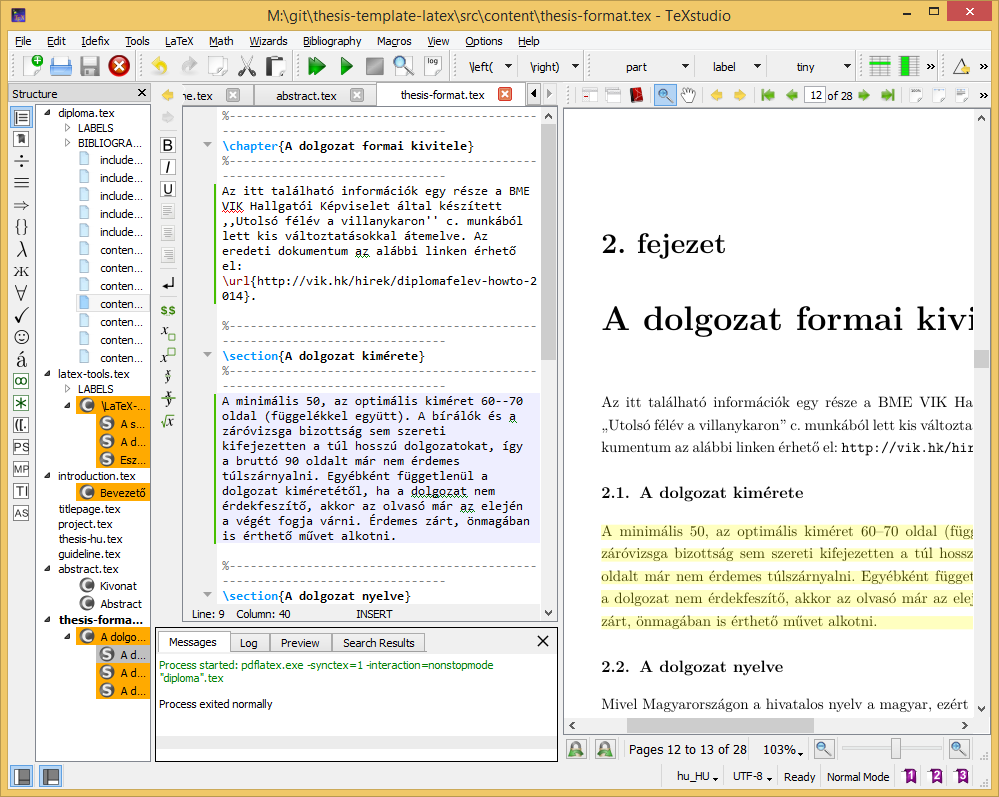
\includegraphics[width=67mm, keepaspectratio]{figures/TeXstudio.png}\hspace{1cm}
	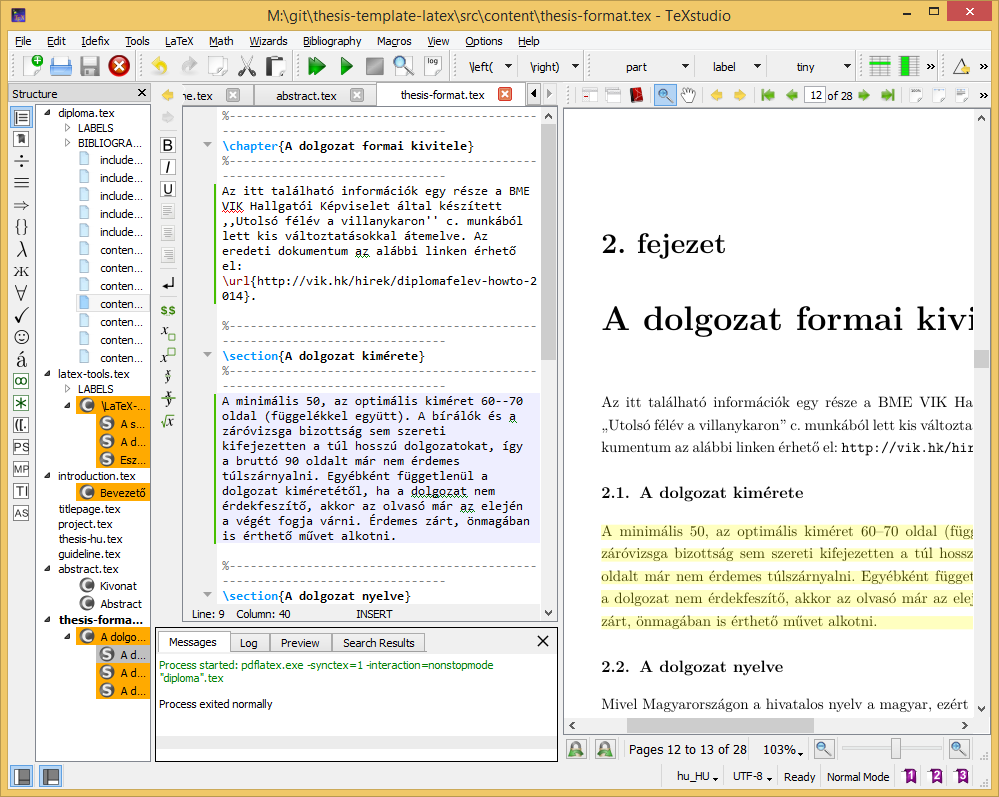
\includegraphics[width=67mm, keepaspectratio]{figures/TeXstudio.png}\\\vspace{5mm}
	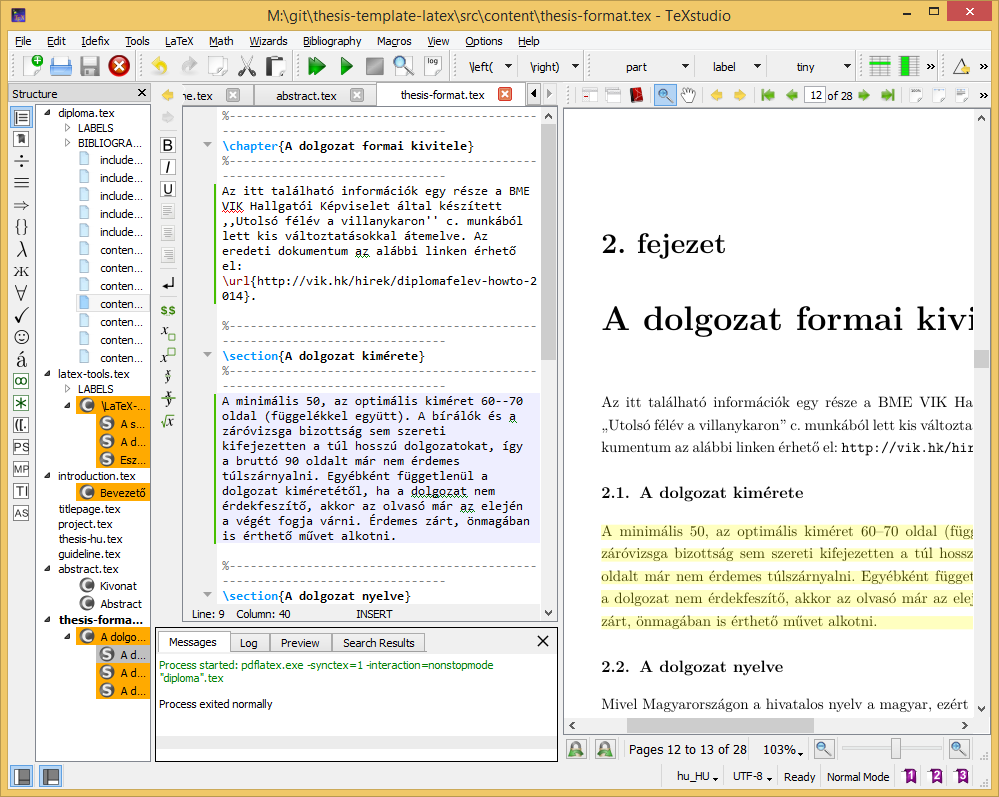
\includegraphics[width=67mm, keepaspectratio]{figures/TeXstudio.png}\hspace{1cm}
	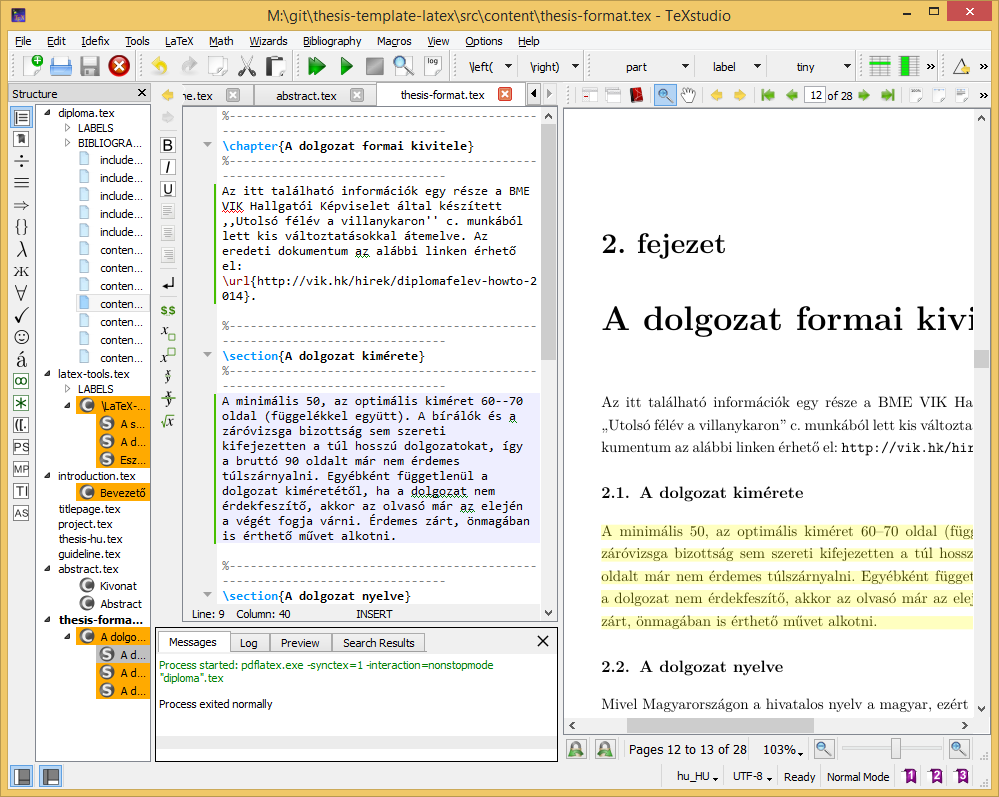
\includegraphics[width=67mm, keepaspectratio]{figures/TeXstudio.png}
	\caption{Több képfájl beillesztése esetén térközöket is érdemes használni.}
	\label{fig:HVSpaces}
\end{figure}

A táblázatok használatára \aref{tab:TabularExample}~táblázat mutat példát. A táblázatok formázásához hasznos tanácsokat találunk a \verb+booktabs+ csomag dokumentációjában.

\begin{table}[ht]
	\footnotesize
	\centering
	\begin{tabular}{ l c c }
		\toprule
		Órajel & Frekvencia & Cél pin \\
		\midrule
		CLKA & 100 MHz & FPGA CLK0\\
		CLKB & 48 MHz  & FPGA CLK1\\
		CLKC & 20 MHz  & Processzor\\
		CLKD & 25 MHz  & Ethernet chip \\
		CLKE & 72 MHz  & FPGA CLK2\\
		XBUF & 20 MHz  & FPGA CLK3\\
		\bottomrule
	\end{tabular}
	\caption{Az órajel-generátor chip órajel-kimenetei.}
	\label{tab:TabularExample}
\end{table}


%----------------------------------------------------------------------------
\section{Felsorolások és listák}
%----------------------------------------------------------------------------
Számozatlan felsorolásra mutat példát a jelenlegi bekezdés:
\begin{itemize}
	\item \emph{első bajusz:} ide lehetne írni az első elem kifejését,
	\item \emph{második bajusz:} ide lehetne írni a második elem kifejését,
	\item \emph{ez meg egy szakáll:} ide lehetne írni a harmadik elem kifejését.
\end{itemize}

Számozott felsorolást is készíthetünk az alábbi módon:
\begin{enumerate}
	\item \emph{első bajusz:} ide lehetne írni az első elem kifejését, és ez a kifejtés így néz ki, ha több sorosra sikeredik,
	\item \emph{második bajusz:} ide lehetne írni a második elem kifejését,
	\item \emph{ez meg egy szakáll:} ide lehetne írni a harmadik elem kifejését.
\end{enumerate}
A felsorolásokban sorok végén vessző, az utolsó sor végén pedig pont a szokásos írásjel. Ez alól kivételt képezhet, ha az egyes elemek több teljes mondatot tartalmaznak.

Listákban a dolgozat szövegétől elkülönítendő kódrészleteket, programsorokat, pszeudo-kódokat jeleníthetünk meg (\ref{lst:Example}.~kódrészlet).
\begin{lstlisting}[language=tex,caption=A fenti számozott felsorolás \LaTeX-forráskódja,label=lst:Example]
\begin{enumerate}
	\item \emph{els(*@ő@*) bajusz:} ide lehetne írni az els(*@ő@*) elem kifejését,
	és ez a kifejtés így néz ki, ha több sorosra sikeredik,
	\item \emph{második bajusz:} ide lehetne írni a második elem kifejését,
	\item \emph{ez meg egy szakáll:} ide lehetne írni a harmadik elem kifejését.
\end{enumerate}
\end{lstlisting}
A lista keretét, háttérszínét, egész stílusát megválaszthatjuk. Ráadásul különféle programnyelveket és a nyelveken belül kulcsszavakat is definiálhatunk, ha szükséges. Erről bővebbet a \verb+listings+ csomag hivatalos leírásában találhatunk.

%----------------------------------------------------------------------------
\section{Képletek}
%----------------------------------------------------------------------------
Ha egy formula nem túlságosan hosszú, és nem akarjuk hivatkozni a szövegből, mint például a $e^{i\pi}+1=0$ képlet, \emph{szövegközi képletként} szokás leírni. Csak, hogy másik példát is lássunk, az $U_i=-d\Phi/dt$ Faraday-törvény a $\rot E=-\frac{dB}{dt}$ differenciális alakban adott Maxwell-egyenlet felületre vett integráljából vezethető le. Látható, hogy a \LaTeX-fordító a sorközöket betartja, így a szöveg szedése esztétikus marad szövegközi képletek használata esetén is.

Képletek esetén az általános konvenció, hogy a kisbetűk skalárt, a kis félkövér betűk ($\mathbf{v}$) oszlopvektort -- és ennek megfelelően $\mathbf{v}^T$ sorvektort -- a kapitális félkövér betűk ($\mathbf{V}$) mátrixot jelölnek. Ha ettől el szeretnénk térni, akkor az alkalmazni kívánt jelölésmódot célszerű külön alfejezetben definiálni. Ennek megfelelően, amennyiben $\mathbf{y}$ jelöli a mérések vektorát, $\mathbf{\vartheta}$ a paraméterek vektorát és $\hat{\mathbf{y}}=\mathbf{X}\vartheta$ a paraméterekben lineáris modellt, akkor a \emph{Least-Squares} értelemben optimális paraméterbecslő $\hat{\mathbf{\vartheta}}_{LS}=(\mathbf{X}^T\mathbf{X})^{-1}\mathbf{X}^T\mathbf{y}$ lesz.

Emellett kiemelt, sorszámozott képleteket is megadhatunk, ennél az \verb+equation+ és a \verb+eqnarray+ környezetek helyett a korszerűbb \verb+align+ környezet alkalmazását javasoljuk (több okból, különféle problémák elkerülése végett, amelyekre most nem térünk ki). Tehát
\begin{align}
\dot{\mathbf{x}}&=\mathbf{A}\mathbf{x}+\mathbf{B}\mathbf{u},\\
\mathbf{y}&=\mathbf{C}\mathbf{x},
\end{align}
ahol $\mathbf{x}$ az állapotvektor, $\mathbf{y}$ a mérések vektora és $\mathbf{A}$, $\mathbf{B}$ és $\mathbf{C}$ a rendszert leíró paramétermátrixok. Figyeljük meg, hogy a két egyenletben az egyenlőségjelek egymáshoz igazítva jelennek meg, mivel a mindkettőt az \& karakter előzi meg a kódban. Lehetőség van számozatlan kiemelt képlet használatára is, például
\begin{align}
\dot{\mathbf{x}}&=\mathbf{A}\mathbf{x}+\mathbf{B}\mathbf{u},\nonumber\\
\mathbf{y}&=\mathbf{C}\mathbf{x}\nonumber.
\end{align}
Mátrixok felírására az $\mathbf{A}\mathbf{x}=\mathbf{b}$ inhomogén lineáris egyenlet részletes kifejtésével mutatunk példát:
\begin{align}
\begin{bmatrix}
a_{11} & a_{12} & \dots & a_{1n}\\
a_{21} & a_{22} & \dots & a_{2n}\\
\vdots & \vdots & \ddots & \vdots\\
a_{m1} & a_{m2} & \dots & a_{mn}
\end{bmatrix}
\begin{pmatrix}x_1\\x_2\\\vdots\\x_n\end{pmatrix}=
\begin{pmatrix}b_1\\b_2\\\vdots\\b_m\end{pmatrix}.
\end{align}
A \verb+\frac+ utasítás hatékonyságát egy általános másodfokú tag átviteli függvényén keresztül mutatjuk be, azaz
\begin{align}
W(s)=\frac{A}{1+2T\xi s+s^2T^2}.
\end{align}
A matematikai mód minden szimbólumának és képességének a bemutatására természetesen itt nincs lehetőség, de gyors referenciaként hatékonyan használhatók a következő linkek:\\
\indent\url{http://www.artofproblemsolving.com/LaTeX/AoPS_L_GuideSym.php},\\
\indent\url{http://www.ctan.org/tex-archive/info/symbols/comprehensive/symbols-a4.pdf},\\
\indent\url{ftp://ftp.ams.org/pub/tex/doc/amsmath/short-math-guide.pdf}.\\
Ez pedig itt egy magyarázat, hogy miért érdemes \verb+align+ környezetet használni:\\
\indent\url{http://texblog.net/latex-archive/maths/eqnarray-align-environment/}.

%----------------------------------------------------------------------------
\section{Irodalmi hivatkozások}
\label{sec:HowtoReference}
%----------------------------------------------------------------------------
Egy \LaTeX~dokumentumban az irodalmi hivatkozások definíciójának két módja van. Az egyik a \verb+\thebibliograhy+ környezet használata a dokumentum végén, az \verb+\end{document}+ lezárás előtt.
\begin{lstlisting}[language=tex]
\begin{thebibliography}{9}

\bibitem{Lamport94} Leslie Lamport, \emph{\LaTeX: A Document Preparation System}.
Addison Wesley, Massachusetts, 2nd Edition, 1994.

\end{thebibliography}
\end{lstlisting}

Ezek után a dokumentumban a \verb+\cite{Lamport94}+ utasítással hivatkozhatunk a forrásra. A fenti megadás viszonylag kötetlen, a szerző maga formázza az irodalomjegyzéket (ami gyakran inkonzisztens eredményhez vezet).

Egy sokkal professzionálisabb módszer a BiB\TeX{} használata, ezért ez a sablon is ezt támogatja. Ebben az esetben egy külön szöveges adatbázisban definiáljuk a forrásmunkákat, és egy külön stílusfájl határozza meg az irodalomjegyzék kinézetét. Ez, összhangban azzal, hogy külön formátumkonvenció határozza meg a folyóirat-, a könyv-, a konferenciacikk- stb. hivatkozások kinézetét az irodalomjegyzékben (a sablon használata esetén ezzel nem is kell foglalkoznia a hallgatónak, de az eredményt célszerű ellenőrizni). felhasznált hivatkozások adatbázisa egy \verb+.bib+ kiterjesztésű szöveges fájl, amelynek szerkezetét a \Aref{lst:Bibtex} kódrészlet demonstrálja. A forrásmunkák bevitelekor a sor végi vesszők külön figyelmet igényelnek, mert hiányuk a BiB\TeX-fordító hibaüzenetét eredményezi. A forrásmunkákat típus szerinti kulcsszó vezeti be (\verb+@book+ könyv, \verb+@inproceedings+ konferenciakiadványban megjelent cikk, \verb+@article+ folyóiratban megjelent cikk, \verb+@techreport+ valamelyik egyetem gondozásában megjelent műszaki tanulmány, \verb+@manual+ műszaki dokumentáció esetén stb.). Nemcsak a megjelenés stílusa, de a kötelezően megadandó mezők is típusról-típusra változnak. Egy jól használható referencia a \url{http://en.wikipedia.org/wiki/BibTeX} oldalon található.

\begin{lstlisting}[caption=Példa szöveges irodalomjegyzék-adatbázisra Bib\TeX{} használata esetén.,label=lst:Bibtex]
@book{Wettl04,
  author    = {Ferenc Wettl and Gyula Mayer and Péter Szabó},
  publisher = {Panem Könyvkiadó},
  title     = {\LaTeX~kézikönyv},
  year      = {2004},
}

@article{Candy86,
  author       = {James C. Candy},
  journaltitle = {{IEEE} Trans.\ on Communications},
  month        = {01},
  note         = {\doi{10.1109/TCOM.1986.1096432}},
  number       = {1},
  pages        = {72--76},
  title        = {Decimation for Sigma Delta Modulation},
  volume       = {34},
  year         = {1986},
}

@inproceedings{Lee87,
  author    = {Wai L. Lee and Charles G. Sodini},
  booktitle = {Proc.\ of the IEEE International Symposium on Circuits and Systems},
  location  = {Philadelphia, PA, USA},
  month     = {05~4--7},
  pages     = {459--462},
  title     = {A Topology for Higher Order Interpolative Coders},
  vol       = {2},
  year      = {1987},
}

@thesis{KissPhD,
  author      = {Peter Kiss},
  institution = {Technical University of Timi\c{s}oara, Romania},
  month       = {04},
  title       = {Adaptive Digital Compensation of Analog Circuit Imperfections for Cascaded Delta-Sigma Analog-to-Digital Converters},
  type        = {phdthesis},
  year        = {2000},
}

@manual{Schreier00,
  author       = {Richard Schreier},
  month        = {01},
  note         = {\url{http://www.mathworks.com/matlabcentral/fileexchange/}},
  organization = {Oregon State University},
  title        = {The Delta-Sigma Toolbox v5.2},
  year         = {2000},
}

@misc{DipPortal,
  author       = {{Budapesti Műszaki és Gazdaságtudományi Egyetem Villamosmérnöki és Informatikai Kar}},
  howpublished = {\url{http://diplomaterv.vik.bme.hu/}},
  title        = {Diplomaterv portál (2011. február 26.)},
}

@incollection{Mkrtychev:1997,
  author    = {Mkrtychev, Alexey},
  booktitle = {Logical Foundations of Computer Science},
  doi       = {10.1007/3-540-63045-7_27},
  editor    = {Adian, Sergei and Nerode, Anil},
  isbn      = {978-3-540-63045-6},
  pages     = {266-275},
  publisher = {Springer Berlin Heidelberg},
  series    = {Lecture Notes in Computer Science},
  title     = {Models for the logic of proofs},
  url       = {http://dx.doi.org/10.1007/3-540-63045-7_27},
  volume    = {1234},
  year      = {1997},
}
\end{lstlisting}

A stílusfájl egy \verb+.sty+ kiterjesztésű fájl, de ezzel lényegében nem kell foglalkozni, mert vannak beépített stílusok, amelyek jól használhatók. Ez a sablon a BiB\TeX-et használja, a hozzá tartozó adatbázisfájl a \verb+mybib.bib+ fájl. Megfigyelhető, hogy az irodalomjegyzéket a dokumentum végére (a \verb+\end{document}+ utasítás elé) beillesztett \verb+\bibliography{mybib}+ utasítással hozhatjuk létre, a stílusát pedig ugyanitt a  \verb+\bibliographystyle{plain}+ utasítással adhatjuk meg. Ebben az esetben a \verb+plain+ előre definiált stílust használjuk (a sablonban is ezt állítottuk be). A \verb+plain+ stíluson kívül természetesen számtalan más előre definiált stílus is létezik. Mivel a \verb+.bib+ adatbázisban ezeket megadtuk, a BiB\TeX-fordító is meg tudja különböztetni a szerzőt a címtől és a kiadótól, és ez alapján automatikusan generálódik az irodalomjegyzék a stílusfájl által meghatározott stílusban.

Az egyes forrásmunkákra a szövegből továbbra is a \verb+\cite+ paranccsal tudunk hivatkozni, így \aref{lst:Bibtex}.~kódrészlet esetén a hivatkozások rendre \verb+\cite{Wettl04}+, \verb+\cite{Candy86}+, \verb+\cite{Lee87}+, \verb+\cite{KissPhD}+, \verb+\cite{Schreirer00}+,
\verb+\cite{Mkrtychev:1997}+ és \verb+\cite{DipPortal}+. Az egyes forrásmunkák sorszáma az irodalomjegyzék bővítésekor változhat. Amennyiben az aktuális számhoz illeszkedő névelőt szeretnénk használni, használjuk az \verb+\acite{}+ parancsot.

Az irodalomjegyzékben alapértelmezésben csak azok a forrásmunkák jelennek meg, amelyekre található hivatkozás a szövegben, és ez így alapvetően helyes is, hiszen olyan forrásmunkákat nem illik az irodalomjegyzékbe írni, amelyekre nincs hivatkozás.

Mivel a fordítási folyamat során több lépésben oldódnak fel a szimbólumok, ezért gyakran többször is le kell fordítani a dokumentumot. Ilyenkor ez első 1-2 fordítás esetleg szimbólum-feloldásra vonatkozó figyelmeztető üzenettel zárul. Ha hibaüzenettel zárul bármelyik fordítás, akkor nincs értelme megismételni, hanem a hibát kell megkeresni. A \verb+.bib+ fájl megváltoztatáskor sokszor nincs hatása a változtatásnak azonnal, mivel nem mindig fut újra a BibTeX fordító. Ezért célszerű a változtatás után azt manuálisan is lefuttatni (TeXstudio esetén \verb+Tools/Bibliography+).

Hogy a szövegbe ágyazott hivatkozások kinézetét demonstráljuk, itt most sorban meghivatkozzuk a \cite{Wettl04}, \cite{Candy86}, \cite{Lee87}, \cite{KissPhD}, \cite{Schreier00} és \acite{Mkrtychev:1997}\footnote{Informatikai témában gyakran hivatkozunk cikkeket a Springer LNCS valamely kötetéből, ez a hivatkozás erre mutat egy helyes példát.} forrásmunkát, valamint \acite{DipPortal} weboldalt.

Megjegyzendő, hogy az ékezetes magyar betűket is tartalmazó \verb+.bib+ fájl az \verb+inputenc+ csomaggal betöltött \verb+latin2+ betűkészlet miatt fordítható. Ugyanez a \verb+.bib+ fájl hibaüzenettel fordul egy olyan dokumentumban, ami nem tartalmazza a \verb+\usepackage[latin2]{inputenc}+ sort. Speciális igény esetén az irodalmi adatbázis általánosabb érvényűvé tehető, ha az ékezetes betűket speciális latex karakterekkel helyettesítjük a \verb+.bib+ fájlban, pl. á helyett \verb+\'{a}+-t vagy ő helyett \verb+\H{o}+-t írunk.

Irodalomhivatkozásokat célszerű először olyan szolgáltatásokban keresni, ahol jó minőségű bejegyzések találhatók (pl. ACM Digital Library,\footnote{\url{https://dl.acm.org/}} DBLP,\footnote{\url{http://dblp.uni-trier.de/}} IEEE Xplore,\footnote{\url{http://ieeexplore.ieee.org/}} SpringerLink\footnote{\url{https://link.springer.com/}}) és csak ezek után használni kevésbé válogatott forrásokat (pl. Google Scholar\footnote{\url{http://scholar.google.com/}}). A jó minőségű bejegyzéseket is érdemes megfelelően tisztítani.\footnote{\url{https://github.com/FTSRG/cheat-sheets/wiki/BibTeX-Fixing-entries-from-common-sources}} A sablon angol nyelvű változatában használt \texttt{plainnat} beállítás egyik sajátossága, hogy a cikkhez generált hivatkozás a cikk DOI-ját és URL-jét is tartalmazza, ami gyakran duplikátumhoz vezet -- érdemes tehát a DOI-kat tartalmazó URL mezőket törölni. 

%----------------------------------------------------------------------------
\section{A dolgozat szerkezete és a forrásfájlok}
%----------------------------------------------------------------------------
A diplomatervsablonban a TeX fájlok két alkönyvtárban helyezkednek el. Az \verb+include+ könyvtárban azok szerepelnek, amiket tipikusan nem kell szerkesztenünk, ezek a sablon részei (pl. címoldal). A \verb+content+ alkönyvtárban pedig a saját munkánkat helyezhetjük el. Itt érdemes az egyes fejezeteket külön \TeX{} állományokba rakni.

A diplomatervsablon (a kari irányelvek szerint) az alábbi fő fejezetekből áll:
\begin{enumerate}
	\item 1 oldalas \emph{tájékoztató} a szakdolgozat/diplomaterv szerkezetéről (\verb+include/guideline.tex+), ami a végső dolgozatból törlendő,
	\item \emph{feladatkiírás} (\verb+include/project.tex+), a dolgozat nyomtatott verzójában ennek a helyére kerül a tanszék által kiadott, a tanszékvezető által aláírt feladatkiírás, a dolgozat elektronikus verziójába pedig a feladatkiírás egyáltalán ne kerüljön bele, azt külön tölti fel a tanszék a diplomaterv-honlapra,
	\item \emph{címoldal} (\verb+include/titlepage.tex+),
	\item \emph{tartalomjegyzék} (\verb+thesis.tex+),
	\item a diplomatervező \emph{nyilatkozat}a az önálló munkáról (\verb+include/declaration.tex+),
	\item 1-2 oldalas tartalmi \emph{összefoglaló} magyarul és angolul, illetve elkészíthető még további nyelveken is (\verb+content/abstract.tex+),
	\item \emph{bevezetés}: a feladat értelmezése, a tervezés célja, a feladat indokoltsága, a diplomaterv felépítésének rövid összefoglalása (\verb+content/introduction.tex+),
	\item sorszámmal ellátott \emph{fejezetek}: a feladatkiírás pontosítása és részletes elemzése, előzmények (irodalomkutatás, hasonló alkotások), az ezekből levonható következtetések, a tervezés részletes leírása, a döntési lehetőségek értékelése és a választott megoldások indoklása, a megtervezett műszaki alkotás értékelése, kritikai elemzése, továbbfejlesztési lehetőségek,
	\item esetleges \emph{köszönetnyilvánítás}ok (\verb+content/acknowledgement.tex+),
	\item részletes és pontos \emph{irodalomjegyzék} (ez a sablon esetében automatikusan generálódik a \verb+thesis.tex+ fájlban elhelyezett \verb+\bibliography+ utasítás hatására, \az+\refstruc{sec:HowtoReference}ban leírtak szerint),
	\item \emph{függelékek} (\verb+content/appendices.tex+).
\end{enumerate}

A sablonban a fejezetek a \verb+thesis.tex+ fájlba vannak beillesztve \verb+\include+ utasítások segítségével. Lehetőség van arra, hogy csak az éppen szerkesztés alatt álló \verb+.tex+ fájlt fordítsuk le, ezzel lerövidítve a fordítási folyamatot. Ezt a lehetőséget az alábbi kódrészlet biztosítja a \verb+thesis.tex+ fájlban.
\begin{lstlisting}
\includeonly{
	guideline,%
	project,%
	titlepage,%
	declaration,%
	abstract,%
	introduction,%
	chapter1,%
	chapter2,%
	chapter3,%
	acknowledgement,%
	appendices,%
}
\end{lstlisting}

Ha az alábbi kódrészletben az egyes sorokat a \verb+%+ szimbólummal kikommentezzük, akkor a megfelelő \verb+.tex+ fájl nem fordul le. Az oldalszámok és a tartalomjegyék természetesen csak akkor billennek helyre, ha a teljes dokumentumot lefordítjuk.

%----------------------------------------------------------------------------
\newpage
\section{Alapadatok megadása}
%----------------------------------------------------------------------------
A diplomaterv alapadatait (cím, szerző, konzulens, konzulens titulusa) a \verb+thesis.tex+ fájlban lehet megadni.

%----------------------------------------------------------------------------
\section{Új fejezet írása}
%----------------------------------------------------------------------------
A főfejezetek külön \verb+content+ könyvtárban foglalnak helyet. A sablonhoz 3 fejezet készült. További főfejezeteket úgy hozhatunk létre, ha új \TeX~fájlt készítünk a fejezet számára, és a \verb+thesis.tex+ fájlban, a \verb+\include+ és \verb+\includeonly+ utasítások argumentumába felvesszük az új \verb+.tex+ fájl nevét.


%----------------------------------------------------------------------------
\section{Definíciók, tételek, példák}
%----------------------------------------------------------------------------

\begin{definition}[Fluxuskondenzátor térerőssége]
Lorem ipsum dolor sit amet, consectetur adipiscing elit, sed do eiusmod tempor incididunt ut labore et dolore magna aliqua. Ut enim ad minim veniam, quis nostrud exercitation ullamco laboris nisi ut aliquip ex ea commodo consequat.
\end{definition}

\begin{example}
Példa egy példára. Duis aute irure dolor in reprehenderit in voluptate velit esse cillum dolore eu fugiat nulla pariatur. Excepteur sint occaecat cupidatat non proident, sunt in culpa qui officia deserunt mollit anim id est laborum.
\end{example}

\begin{theorem}[Kovács tétele]
Duis aute irure dolor in reprehenderit in voluptate velit esse cillum dolore eu fugiat nulla pariatur. Excepteur sint occaecat cupidatat non proident, sunt in culpa qui officia deserunt mollit anim id est laborum.
\end{theorem}



% Acknowledgements
%~~~~~~~~~~~~~~~~~~~~~~~~~~~~~~~~~~~~~~~~~~~~~~~~~~~~~~~~~~~~~~~~~~~~~~~~~~~~~~~~~~~~~~
%----------------------------------------------------------------------------
\chapter*{\koszonetnyilvanitas}\addcontentsline{toc}{chapter}{\koszonetnyilvanitas}
%----------------------------------------------------------------------------

Ez nem kötelező, akár törölhető is. Ha a szerző szükségét érzi, itt lehet köszönetet nyilvánítani azoknak, akik hozzájárultak munkájukkal ahhoz, hogy a hallgató a szakdolgozatban vagy diplomamunkában leírt feladatokat sikeresen elvégezze. A konzulensnek való köszönetnyilvánítás sem kötelező, a konzulensnek hivatalosan is dolga, hogy a hallgatót konzultálja.


% List of Figures, Tables
%~~~~~~~~~~~~~~~~~~~~~~~~~~~~~~~~~~~~~~~~~~~~~~~~~~~~~~~~~~~~~~~~~~~~~~~~~~~~~~~~~~~~~~
%\listoffigures\addcontentsline{toc}{chapter}{\listfigurename}
%\listoftables\addcontentsline{toc}{chapter}{\listtablename}


% Bibliography
%~~~~~~~~~~~~~~~~~~~~~~~~~~~~~~~~~~~~~~~~~~~~~~~~~~~~~~~~~~~~~~~~~~~~~~~~~~~~~~~~~~~~~~
\addcontentsline{toc}{chapter}{\bibname}
\bibliography{bib/mybib}


% Appendix
%~~~~~~~~~~~~~~~~~~~~~~~~~~~~~~~~~~~~~~~~~~~~~~~~~~~~~~~~~~~~~~~~~~~~~~~~~~~~~~~~~~~~~~
%----------------------------------------------------------------------------
\appendix
%----------------------------------------------------------------------------
%\chapter*{\fuggelek}\addcontentsline{toc}{chapter}{\fuggelek}
%\setcounter{chapter}{\appendixnumber}
%\setcounter{equation}{0} % a fofejezet-szamlalo az angol ABC 6. betuje (F) lesz
%\numberwithin{equation}{section}
%\numberwithin{figure}{section}
%\numberwithin{lstlisting}{section}
%\numberwithin{tabular}{section}

%----------------------------------------------------------------------------
\chapter{LTL Expressions}
%----------------------------------------------------------------------------

%----------------------------------------------------------------------------
\section{The Syntax of the LTL Expressions}
%----------------------------------------------------------------------------
\begin{lstlisting} [language=tex,caption=Full syntax of the LTL expressions using the EBNF notation \cite{EBNFStandard},label=lst_ltlfullsyntax]
	LTLExpression = ArrowExpression;
	ArrowExpression = (OrExpression '->' ArrowExpression) |
	                    (OrExpression '<->' ArrowExpression) |
	                     OrExpression;
	OrExpression = (OrExpression '|' AndExpression) |
	                  AndExpression;
	AndExpression = (AndExpression '&' UntilExpression) |
	                   UntilExpression;
	UntilExpression = (FutureGloballyExpression 'U' UntilExpression) |
	                     FutureGloballyExpression;
	FutureGloballyExpression = ('F' NextExpression) |
	                             ('G' NextExpression) |
	                              NextExpression;
	NextExpression = ('X' PrimaryExpression) |
	                    PrimaryExpression;
	PrimaryExpression = ('(' LTLExpression ')') |
	                      ('!' PrimaryExpression) |
	                       LiteralExpression;
	LiteralExpression = AtomicProposition |
	                      'true' |
	                      'false';
	AtomicProposition = '^'?('a-z'|'A-Z'|'_') ('a-z'|'A-Z'|'_'|'.'|'0-9')*;		
\end{lstlisting}

%----------------------------------------------------------------------------
\clearpage\section{Pedestrian Crossing}
%----------------------------------------------------------------------------
\bigskip
\begin{lstlisting} [language=tex,caption=A possible run of the learning process,label=lst_examplelearning]
	Unknown output for input sequence: [trafficControl_interrupt]
	Would you like to specify the output through an (I)O pair, an (L)TL expression, a (V)alid Trace or an I(N)valid Trace?
	>I
	Please provide the expected output:
	>TrafficDisplay.blinkingYellow
	Unknown output for input sequence: [trafficControl_interrupt, trafficControl_interrupt]
	Would you like to specify the output through an (I)O pair, an (L)TL expression, a (V)alid Trace or an I(N)valid Trace?
	>V
	Please provide a valid trace:
	>TrafficControl.interrupt/trafficDisplay.blinkingYellow TrafficControl.interrupt/TrafficDisplay.red TrafficControl.interrupt/TrafficDisplay.blinkingYellow TrafficControl.interrupt/TrafficDisplay.red
	Unknown output for input sequence: [trafficControl_toggle, trafficControl_interrupt]
	Would you like to specify the output through an (I)O pair, an (L)TL expression, a (V)alid Trace or an I(N)valid Trace?
	>I
	Please provide the expected output:
	>TrafficDisplay.blinkingYellow
	Unknown output for input sequence: [trafficControl_toggle, trafficControl_interrupt, trafficControl_interrupt]
	Would you like to specify the output through an (I)O pair, an (L)TL expression, a (V)alid Trace or an I(N)valid Trace?
	>I
	Please provide the expected output:
	>TrafficDisplay.red
	Unknown output for input sequence: [trafficControl_toggle, trafficControl_toggle, trafficControl_interrupt]
	Would you like to specify the output through an (I)O pair, an (L)TL expression, a (V)alid Trace or an I(N)valid Trace?
	>I
	Please provide the expected output:
	>TrafficDisplay.blinkingYellow
	Unknown output for input sequence: [trafficControl_toggle, trafficControl_toggle, trafficControl_interrupt, trafficControl_interrupt]
	Would you like to specify the output through an (I)O pair, an (L)TL expression, a (V)alid Trace or an I(N)valid Trace?
	>I
	Please provide the expected output:
	>TrafficDisplay.red
	Unknown output for input sequence: [trafficControl_toggle, trafficControl_toggle, trafficControl_toggle, trafficControl_interrupt]
	Would you like to specify the output through an (I)O pair, an (L)TL expression, a (V)alid Trace or an I(N)valid Trace?
	>I
	Please provide the expected output:
	>TrafficDisplay.blinkingYellow
	Equivalence Query. Please provide a counterexample if exists.
\end{lstlisting}


%\label{page:last}
\end{document}
